\documentclass[conference,twocolumn,a4paper]{IEEEtran}
\IEEEoverridecommandlockouts
% The preceding line is only needed to identify funding in the first footnote. If that is unneeded, please comment it out.
\usepackage{cite}
\usepackage{amsmath,amsfonts,amssymb,amsthm}
\usepackage{algorithmic}
\usepackage{graphicx}
\usepackage{textcomp}
\usepackage{xcolor}
\usepackage[utf8]{inputenc}
\usepackage{commath}
\usepackage{scalerel}
\usepackage{tikz}
\usepackage[]{changes}
\usepackage{caption}
\usepackage{subcaption}
\usepackage{layouts}
\usepackage[draft]{hyperref}
% \usepackage{nohyperref}  % This makes hyperref commands do nothing without errors

% tools for tikzplot
\usepackage{pgfplots}
\DeclareUnicodeCharacter{2212}{−}
\usepgfplotslibrary{groupplots,dateplot}
\usetikzlibrary{patterns,shapes.arrows}
\pgfplotsset{compat=newest}

% custom legend
% https://tex.stackexchange.com/questions/278530/how-i-can-customize-a-legend-on-pgfplots

% https://tex.stackexchange.com/questions/84127/correctly-align-vertical-text-on-a-baseline-in-pgfplots
\def\mystrut{\vphantom{hg}}

% https://tex.stackexchange.com/questions/204395/add-custom-entry-into-legend-in-pgfplot
\pgfplotsset{
    legend image with text/.style={
        legend image code/.code={%
            \node[anchor=center] at (0.3cm,0cm) {#1};
        }
    },
}


\newcommand{\ac}[1]{{\color{teal}[Achiel: #1]}}
\newcommand{\zh}[1]{{\color{blue}[Genia: #1]}}
\newcommand{\sofie}[1]{{\color{red}[Sofie: #1]}}

\def\BibTeX{{\rm B\kern-.05em{\sc i\kern-.025em b}\kern-.08em
    T\kern-.1667em\lower.7ex\hbox{E}\kern-.125emX}}
    

\begin{document}

\title{
%Reliable Cellular UAV Communication Using Multi-Operator Diversity and Sidelobe Boosting; 
Drone delivery: Reliable Cellular UAV Communication Using Multi-Operator Diversity% and Sidelobe Boosting%; 
%Reliable Cellular Communication for UAV-based Delivery Using Multi-Operator Diversity and Sidelobe Boosting\\
\thanks{This research is supported by the Research Foundation Flanders (FWO), projects no. S003817N (OmniDrone) and G098020N.}
}

% \author{\IEEEauthorblockN{1\textsuperscript{st} Given Name Surname}
% \IEEEauthorblockA{\textit{dept. name of organization (of Aff.)} \\
% \textit{name of organization (of Aff.)}\\
% City, Country \\
% email address or ORCID}
% \and
% \IEEEauthorblockN{2\textsuperscript{nd} Given Name Surname}
% \IEEEauthorblockA{\textit{dept. name of organization (of Aff.)} \\
% \textit{name of organization (of Aff.)}\\
% City, Country \\
% email address or ORCID}
% \and
% \IEEEauthorblockN{3\textsuperscript{rd} Given Name Surname}
% \IEEEauthorblockA{\textit{dept. name of organization (of Aff.)} \\
% \textit{name of organization (of Aff.)}\\
% City, Country \\
% email address or ORCID}
% }

\author{\IEEEauthorblockN{
Achiel Colpaert, %\orcidicon{0000-0003-1238-2002},
Micha\"el Raes,
Evgenii Vinogradov, %\orcidicon{0000-0002-4156-0317},
and Sofie Pollin %\orcidicon{0000-0002-1470-2076}
}
\IEEEauthorblockA{KU Leuven, ESAT - Department of Electrical Engineering, Kasteelpark Arenberg 10, 3001 Heverlee, Belgium\\
E-mail: \{achiel.colpaert, evgenii.vinogradov, sofie.pollin\}@kuleuven.be} michael.raes@student.kuleuven.be}

\maketitle

\begin{abstract}
%\ac{rewrite abstract}The advance Unmanned Aerial Vehicles (UAVs), also known as drones, is unstoppable these days, especially now \ac{commercially available wording}. They are also being used professionally in many different sectors for increasingly innovative applications, ranging from inspection and security to local package delivery. However, when moving to beyond visual line of sight (BVLOS) applications, the drone must be assured of a stable and reliable communication link with the operator or with an Unmanned Traffic System in the case of fully autonomous applications. The existing cellular mobile network is a good candidate because of its very widespread coverage. However, research has indicated that existing cellular networks, which are built and optimised for ground users, show very different behaviour in aerial applications. Various works proposed already a range of possible solutions however these mostly require modifying or adding infrastructure or require very complex path planning. Very little work has been done in practical mobile scenarios and this is where this work will make an effort to shine some light\ac{this needs to change}. This work investigates whether a simple solution can be found in connecting to multiple mobile networks simultaneously. Propagation simulations based on real-world mobile network deployment data are the basis for looking at different aspects of network quality. The results confirm the application of network diversity can significantly improve coverage in urban areas and reduce the size of the outage zones. In addition, a hypothetical network applying sidelobe boosting is considered, which can result in an even greater improvement between certain heights. Finally, it is shown that the number of handovers and radio link failures is dramatically reduced when two networks are combined.
The market size of Unmanned Aerial Vehicles (UAVs, a.k.a drones) can reach up to 10\% of the global market value. In particular, drone delivery is one of the most attractive applications. The growing number of drones requires appropriate traffic management systems that will rely on cellular networks. However, it has been shown in the literature that these networks cannot provide reliable communication due to low coverage probability and frequent handovers. This article presents a potential solution targeting these problems while requiring no modifications of the existing infrastructure. Namely, equipping the UAV with multiple cellular modems to connect to different providers' networks introduces network diversity resulting in 98\% coverage probability at the flight altitude of 100 meters. In contrast, one network ensures only 80\% coverage. At the same time, the size of the outage zones becomes up to ten times smaller and the frequency of harmful handovers is reduced to zero. The results are obtained with a physical-layer simulator utilizing a real urban 3D environment, cellular network parameters (e.g., site locations, antenna orientation and gains), and specific aerial channel models.
\end{abstract}

\begin{IEEEkeywords}
UAV, UTM, Urban Air Mobility, Reliability, Cellular networks
\end{IEEEkeywords}

\section{Introduction}
 In May 2021, Morgan Stanley released a forecast \cite{MS} stating that by 2050 the total market of Urban Air Mobility (UAM, including drone delivery, air taxi, patrolling drones, to name a few) will reach up to 11\% of the projected global Gross Domestic Product (GDP). The same document claims that the large-scale deployments of drone-based urban delivery are expected to be in place by 2030. 
 
Apart from the mobility, Unmanned Aerial Vehicles and Systems (UAVs, UASs) are expected to play an essential role in future 6G networks where aerial Base Stations (BSs) will provide connectivity to ground users \cite{Tut18, azari2021evolution, UAV_6G}. Shorter-term predictions say that by 2025, the drone services market will be worth a total of USD 63.6 billion \cite{business2021drone} and the UAV fleet, both recreational and commercial, is projected to reach 2 to 3 million by 2023 \cite{faa2019prediction}.

Managing such a large fleet requires the design of UAS Traffic Management (UTM) solutions in order to ensure expected levels of safety, security, operation transparency, and airspace usage efficiency \cite{Dr_Tech}. The UTM framework formulated by International Civil Aviation Organization (ICAO) in \cite{ICAO} includes cellular technology as a critical enabler of large-scale drone deployments. Several competing UTM implementations have been proposed \cite{Bauranov}. All of them rely on the existence of a reliable command and control (C2) link. Indeed, cellular networks are an ideal candidate as they provide ubiquitous coverage and remove the need for the UTM provider to deploy expensive dedicated wireless infrastructure. 3GPP has taken the first steps to introduce aerial vehicles some time ago now \cite{3gpp2018enhanced}, but many questions remain open \cite{Tut18, UAV_6G}.

\subsection{State of the Art: overview of open problems}
\par In an effort to evaluate the performance of UAVs in cellular networks many different types of studies have been performed, from analysis to simulator based, to actual experimental work. Several relevant overviews can be found in \cite{Tut18, azari2021evolution}. In this article, let us provide just a few of the most relevant works.  

An in-depth analysis of the performance of UAVs in a cellular network based on stochastic geometry provided in \cite{azari2019cellular}. Authors of \cite{rodriguez2021air} and \cite{bertold} characterized the UAV channels through dedicated measurement campaigns. All works listed above conclude that the antenna configuration at BSs should be considered when introducing aerial users to a cellular network as the antennas are pointed towards the ground generally. 

Other simulation-based research has proven that current LTE networks do not provide sufficient coverage at altitudes above building height, mainly due to interference problems \cite{colpaert2018aerial} and high handover rates \cite{colpaert2020beamforming}. Several measurement campaigns \cite{gharib2021exhaustive, Fakhreddine2019HandoverCF} showed satisfying results both in terms of coverage and handover rates. However, they were performed in rural areas where the BS density is much lower compared to an urban scenario. 

\textbf{Takeaways:} A high density of base stations results in high signal strengths but simultaneously high interference levels due to line-of-sight conditions. Moreover, the BS antennas are downtilted to optimize the ground coverage. Consequently, the problem of achieving a highly reliable connection with UAVs in an urban environment remains open due to i) limited coverage caused by high interference (growing with increasing flight altitude); ii) frequent handovers. 
\subsection{Multi-Operator Diversity as a Potential Solution}
This article suggests a solution to increase the reliability of UAV communication links while requiring no modifications of the terrestrial cellular networks. Several studies have shown through network level measurements that equipping a UAV with multiple LTE modems to connect to different providers' networks will improve reliability and Quality of Service \cite{amorim2019improve,sae2020reliability,bacco2022airtoground}. Thus, we can assume that introducing network diversity improves the coverage and handover rates experienced by UAVs. Indeed, network infrastructure from different providers is deployed at different base station sites in the city\footnote{Even when the sites are shared (for instance the same mast can be used), the sector antennas are usually pointed differently. This is due to the need to optimize the performance under different underlying network topology.}. This feature reduces the probability of having a bad connection to all BSs at a given location of UAV. 

The price to pay is a slightly higher payload weight since the modern modems are quite compact. The size and weight can be reduced even further if a dedicated multi-connection module is designed. Another factor is an increased power consumption. However, a more stable connection results in less frequent modifications of the flight path \cite{7888557, Sibren19}. Note that power consumption of the communication modems is negligible in comparison with the propulsion energy \cite{7888557}.
%\paragraph{BS antenna sidelobes boosting} unfortunately, the effect of antenna sidelobe suppression, a feature implemented in many directive cellular antennas, is often ignored in the UAV-related literature. In this work, we investigate i) the influence of sidelobe suppression and ii) assess the possible effect of boosting the gain of sidelobes pointing upwards.
\subsection{Contributions}
The main contributions of this work are:
\begin{enumerate}
    \item We designed a realistic simulator taking into account
    \begin{itemize}
        \item real 3D environment including information about i) ground surface, ii) buildings and infrastructure;
        \item real cellular network parameters (e.g., BS locations, sector orientations, used power, etc.) reported by the Belgian operators to the government;
        \item 3D antenna patterns (with adaptable sidelobes);
        \item specific UAV channel models;
        \item users' mobility (UAVs).
    \end{itemize}
    \item We assessed potential effects of multi-operator diversity on i) coverage and ii) handovers.
%    \item We assessed the effects of sidelobe suppression and boosting on the achievable coverage.
\end{enumerate}
Note that in this work, we focus on a promising use case of drone delivery. UAV delivery will probably be performed at higher altitudes than other popular operations (e.g., patrolling) due to safety reasons. Though the higher altitude can result in more severe damage in case of malfunction, it gives a better time margin for the safety systems to act. For this reason we use altitudes higher than foreseen in \cite{ICAO}. Of course, the presented results are useful for other UAV applications when only the appropriate altitudes are analyzed.
% \subsection{Background}
% \par First sentence, drones are cool.\sofie{maybe remove that first sentence?} Drones are deployed for a large variety of applications, ranging from inspection of buildings\cite{elia2021drone}, to precision agriculture, to aerial basestations or relays \cite{azari2021evolution}, to maybe the most appealing, drone deliveries. Where a UAV will fly from a central depot straight to your doorstep to deliver a package, not prone to any traffic and simultaneously reducing traffic. Especially in large cities where traffic is a problem and the distance to travel is relatively small, drone delivery could be a real improvement to quality of life in big cities. It is predicted that by 2025, the drone services market will be worth a total of USD 63.6 billion \cite{business2021drone} and the UAV fleet, both recreational and commercial, is projected to reach 2 to 3 million by 2023 \cite{faa2019prediction}. One of the main concerns in UAV operation is the safety of operation which can only be guaranteed by a reliable system. In this context Unmanned Traffic Management (UTM) platforms are being developed to increase safety for everyone using the airspace \cite{faa2021unmanned}. Cellular networks are an ideal candidate as they provide ubiquitous coverage and remove the need for the operator to deploy expensive wireless infrastructure. 3GPP has taken the first steps to introduce aerial vehicles some time ago now \cite{3gpp2018enhanced}, but many questions remain open.

% \subsection{State of the Art}
% \par In an effort to evaluate the performance of UAVs in cellular networks many different types of studies have been performed, from analysis to simulator based, to actual experimental work. Azari et al. \cite{azari2019cellular} provides an in-depth analysis of the performance of UAVs in a cellular network based on stochastic geometry \cite{azari2019cellular}. Authors of \cite{rodriguez2021air} characterized the channel of low altitude UAVs through a dedicated measurement campaign. Both works conclude that the antenna configuration at the basestation should be considered when introducing aerial users to a cellular network as the antennas are pointed towards the ground generally. Other simulation based research has proven that current LTE networks do not provide sufficient coverage at altitudes above building height, mainly due to interference problems \cite{colpaert2018aerial} and high handover rates \cite{colpaert2020beamforming}. A measurement campaign in \cite{mohammed2021exhaustive} showed promising results both in terms of coverage and handover rates, however it was performed in a rural area where the basestation density is much lower compared to an urban scenario. 
% \subsection{Hypothesis}
% \par The problem of achieving high reliability \sofie{highly reliable?} UAV networks in an urban environment remains an open problem. A high density of basestations results in high signal strengths but simultaneously high interference levels due to line-of-sight conditions. However, network infrastructure from different telecom providers are deployed at different basestation sites in the city \sofie{is there not a lot of site sharing?}. We hypothesize that by equipping the UAV with multiple LTE modems to connect to different provider's networks we can introduce network diversity to improve both the coverage and handover rates for UAVs.
% \par Another aspect influencing the aerial cover are the basestation antennas as \cite{azari2019cellular,rodriguez2021air} have shown, they point mainly at the downward tilt of the antennas \sofie{strange sentence?}. However, we theorize that the effect of antenna sidelobe suppression, a feature implemented in many directive cellular antennas, is not to be underestimated and reducing this feature could already improve the coverage situation for UAVs.
% \par By introducing these solutions in the current and upcoming cellular networks we can increase the reliability and safety of drone delivery and other services. 
% \subsection{Contributions}
% \par The contributions of this work are as follows \ac{draft}:
% \begin{enumerate}
%     \item Simulations in a realistic scenario to estimate actual performance of the system
%     \item Coverage and how it will be improved through macro network diversity
%     \item Show effect of sidelobe suppression on coverage
%     \item Handovers and how they can be improved through Macro network Diversity
% \end{enumerate}


% \section{section title}
% \par To be able to simulate the received powers, the physical layer simulator developed in \cite{} is used. Once the received power for all sectors is known, one can determine the cell allocation and SINR from this. \ac{requirements for simulation}
% \par Firstly there's a need for terrain and surface information, as this will influence the heights of the antennas and, more importantly, allow us to determine if a sector is in LOS with a point. For this, the DHMV-dataset \cite{} is used and \ac{can be seen in Figure ...}
% \par Secondly, information about the location of the different basestations, their sectors, tilts, transmit powers and antennas needs to be known. For this, a custom \ac{python} script was developed that combines information from the Antenna Registry of the BIPT \cite{}, with the database of \textit{declarations of conformity} issued by operators for each antenna site. These declaration documents contain all necessary information and are parsed to extract the data to a JSON file as input for the simulations.
% \par Thirdly an antenna pattern was simulated that corresponds an antenna that is used on cellular basestation sites in the evaluated area \cite{}. Important to note is that just like the actualla anteann, this simulated sector antenna has sidelobe suppression, which improves power efficiency for serving ground users by reducing energy emitted towards the sky.
% \par Finally, the channel model for aerial vehicles defined by 3GPP in \cite{} is used.
% \par Using this input and the general parameters defined in \ac{table I}, the simulator can evaluate the channel model for 3D point in the simulation area, and as such can calculate the received power from each sector.
\section{Model}
\label{sec:model}

\par To model the scenario of drone deliveries, we consider drones flying in an urban environment at a fixed speed. They travel at constant altitudes ranging from just above rooftop level up to a maximum of 300~m above ground level. They fly in a straight line starting at a random point $A$ in the city to another random point $B$ representing the delivery address. The requirements for a network supporting these drones are twofold. On one side, only a low throughput link is necessary to monitor and control the UAV from a remote location. The requirement for this is a minimum Signal-to-Noise-Ratio (SINR). On the other hand, the link needs to be very reliable. Due to safety concerns, one cannot afford to lose connection to the UAV. The amount of handovers (HO) between sectors and radio link failures (RLF) will affect the time that the UAV is not connected to the network.
\par For the location of our study, we choose the city of Leuven as the environment as this is the location of our university, and this allows us to verify our results even further in the future.
\par We will evaluate the performance of the network using several metrics based on the SINR which is calculated at any 3D point $\vec{p}$ in the simulator as follows: \begin{equation}
	\label{eq:sinr_interference_noise}
	SINR (\vec{p}) = \frac{P_r(\vec{p},a)}{\sum^{A}_{i \neq a} P_{r, i}(\vec{p}) + N},
\end{equation}
where $A$ represents the set of all sectors in the environment and $a$ represents the currently assigned sector, $N$ represents the noise power and is calculated as follows $N = BN_0F$, where $B$ is the bandwidth, $N_0$ is the noise density and $F$ is the noise figure. 
\par The metrics considered are the following: the first being coverage probability $P_{cov}$ calculated as the ratio of the area where the Signal-to-Interference-and-Noise-Ratio (SINR) is larger than a threshold (T) based on throughput requirements, $SINR > T$, divided by the total area. The second metric is the size of the largest continuous zone where no coverage exists in square kilometers, called the maximum outage zone $OUT_{max}$. This metric represents the importance of continuous coverage, large regions of outage results in the UAV being disconnected for long periods of time which is detrimental in a reliable network.

\section{Simulations}
\par To simulate the received powers at any 3D point, an improved version of the physical layer simulator developed in \cite{colpaert2018aerial, colpaert2020beamforming} is used. It uses a real 3D environment based on surface scans to create a virtual environment where assets like base stations and users can be deployed in a 3D space. The modified version includes realistic cellular network configurations as we detail in the following subsection.
\subsection{Environment}
The simulator requires several parameters based on the real world environment as input. First of all, terrain and surface information is required, as this affects the heights of the antennas and, more importantly, allows us to determine if a sector is in line of sight with a point. For this, the DHMV-dataset, see \cite{colpaert2018aerial}, is used and the considered environment is displayed in Fig.~\ref{fig:leuven_dsm_sectors}.

\begin{figure}
	\centering
    \includegraphics[scale=0.6]{img/leuven/env.pdf}
    % \input{img/leuven/env}
	\caption{Digital Surface Model with sectors and simulation area indicated in red. The lines represent the sectors and their azimuth rotation and each color represents a different network.}
	\label{fig:leuven_dsm_sectors}
\end{figure}

\par Secondly, information about the location of the different base stations, their sectors, tilts, transmit powers and antennas needs to be known. For this, information from the Belgian Antenna Registry of the BIPT \cite{bipt-ant}, the organisation managing the spectrum in this environment, is combined with the database of \emph{declarations of conformity} issued by operators for each antenna site. These declaration documents contain all information about the hardware deployed at each antenna site and are used as input for the simulator.

\par Thirdly, we used a 3D antenna pattern  corresponding to the antennas used on the sites in the evaluated area \cite{huaweiantenna}. It is important to note that just like the real antenna, this antenna pattern has sidelobe suppression implemented meaning that the actual gain of the sidelobes is further reduces to improve power efficiency by reducing energy emitted towards the sky. %Later in this study we will evaluate the effect of this sidelobe suppression on the performance of the network for aerial vehicles. Sidelobe suppression is implemented as a relative gain reduction of the sidelobes compared to the maximum gain of the main lobe.

\par Lastly, the used channel model is defined in \cite{3gpp2018enhanced} specifically for aerial vehicles.

\subsection{Scenarios}
\par Two different scenarios are simulated. One static scenario where all points on the map are evaluated at different altitudes, generating statistics of the area at different heights. Secondly, a mobile scenario is evaluated where a UAV travels a random path over the city populated by static ground users. In this scenario, we can evaluate handover behaviour and Radio-Link-Failure (RLF) occurrences of the network.

\subsubsection{Static scenario}

\par The first scenario's goal is to evaluate the statistics of the chosen city of Leuven and characterize the cellular network at different altitudes above ground level to give us some insight on how well a UAV can utilize the cellular network. Using the info of the environment and the general parameters used in a typical LTE deployment, see Table \ref{tab:general_simparams}, the simulator evaluates the channel model for every 3D point in the simulation area, and as such can calculate the received power from each sector at each 3D point. This happens for three different network operators (Op1, Op2 \& Op3). The base station sites of these operators can coincide. The received power from all sectors can be used to determine cell allocation and SINR levels. SINR levels can then be further used to calculate coverage.

\par This characterization of the environment is performed for different operators. After combining all data, we can calculate the SINR at any point in a multi-operator network, as in \cite{nguyen2017using}:
\begin{equation}
	\label{eq:sinr_max}
	SINR (\vec{p}) = \max\limits_{k}\Bigg(\frac{P_r(\vec{p},a)}{\sum^{A}_{i_k \neq a} P_{r, i_k}(\vec{p}) + N}\Bigg),
\end{equation}
where $k$ is the operator index. These SINR values can then be used to calculate the coverage as described in Section \ref{sec:model}. Using all the datapoints at a specific altitude we can also evaluate the area size of continuous outage zones and we can calculate the largest outage zone, $OUT_{max}$.

%\par By swapping out the used antenna patterns in this scenario, we can evaluate the effect of the sidelobe suppression. By inserting antenna patterns without sidelobe suppression and even with sidelobe boosting, we can easily see if it results in an improvement as we hypothesize.

\begin{table}[h!]
	\begin{center}
	  \caption{Simulation Parameters}
	  \label{tab:general_simparams}
	  \begin{tabular}{|l|c|} % <-- Alignments: 1st column left, 2nd middle and 3rd right, with vertical lines in between
		\hline
		\textbf{Parameter} & \textbf{Value}\\
		\hline
		Simulation area, & $9~km^2$\\
		Resolution, & $5~m$\\
		Carrier frequency, $f_c$& $1800~MHz$\\
		Bandwidth, $B$ & $20~MHz$\\
		Outage-threshold, $T$ & $-6~dB$\\
		Noise density, $N_0$ \cite{3gppRadioFrequencyRF2018} & $-174~dBm/Hz$\\
		Noise number, $F$ \cite{3gppRadioFrequencyRF2018} & $9~dB$\\
		\hline

	  \end{tabular}
	\end{center}
  \end{table}
  
\subsubsection{Mobile scenario}

\par Finally a second scenario is simulated to get more insight into the mobility characteristics of a multi-network approach. In \cite{colpaert2020beamforming}, the simulator was extended with the possibility to consider a moving drone that travels over a certain trajectory in three dimensional space and can hence experience changing network circumstances. They also implemented a simplified handover mechanism based on the \verb+A3+-event from the 4G- and 5G standards \cite{3gpp2021NR}.

\par Alongside the handover event, there exists another event that could cause temporary disconnection and latency issues, the
RLF event. When the UE detects problems in the connection it will wait for a specific timer (\verb+T310+ \cite{3gpp2021NR}) to run out and when the problem is not resolved at that time the UE will consider itself in RLF and begin the cell selection procedure again. The handover threshold and the RLF timer are network parameters that the operator can tweak on a per-UE basis. Because we want very low latency for drone applications, the following simulation uses a \verb+T310+ of $200~ms$. For the A3-threshold we take $-2~dB$ as in \cite{3gpp2018enhanced}.

\par In a multi-network context the definitions are slightly different. First, a RLF is defined as an event when the user is not connected to any network. Secondly, a handover is defined as:
\begin{itemize}
	\item One of the used networks has a HO and the other used networks are in RLF at that time;
	\item All used networks experience a handover within 1 second.
\end{itemize}
This period of $1~s$ is self-defined and is a measure for how robust one wants to protect the combined link against near simultaneous handovers. A longer period gives more margin, a shorter period assumes that the handover is correctly resolved when the other network starts a handover. The remainder of the simulation parameters can be found in Table \ref{tab:leuven_ho_stats}, refer to \cite{colpaert2020beamforming} for the full explanation of all the parameters.

\begin{table}[h!]
	\begin{center}
	  \caption{Handover Simulation Parameters}
	  \label{tab:leuven_ho_stats}
	  \begin{tabular}{|l|c|} % <-- Alignments: 1st column left, 2nd middle and 3rd right, with vertical lines in between
		\hline
		\textbf{Parameter} & \textbf{Value}\\
		\hline
		Heights (AGL) $h$  & $20$~m, $40$~m, $80$~m, $160$~m\\
		Drone velocity $v$  & $15~m/s$\\
		Outage-threshold $T$ & $-6~dB$\\
		A3 - Offset $T_{A3}$ & $2~dB$\\
		RLF-timer \verb+T310+ & $200~ms$\\
		Simulation timestep $\delta_t$ & $100~ms$\\
		Number simulations & $5000$ \\
		\hline

	  \end{tabular}
	\end{center}
  \end{table}

\section{Results}

\par In this section, we look at the results generated by the simulations described above. We evaluate the metrics at different altitudes to get a better insight into the effect of drone height. We also draw the evaluations under different network loads, but we focus on the $100~\%$ network load as this is the worst-case scenario but the most important scenario when looking at the reliability of the communication link.
\par First, we evaluate the coverage situation, followed by a study of the effects of using multiple operators. % and of the sidelobe suppression at the antennas. 
Next, we evaluate the handover results and verify whether using multiple networks results in an improvement in terms of handovers.

\subsection{Coverage}
\begin{figure}[]
    \centering % <-- added
	 \resizebox{0.9\linewidth}{!}{
    % This file was created by tikzplotlib v0.9.4.
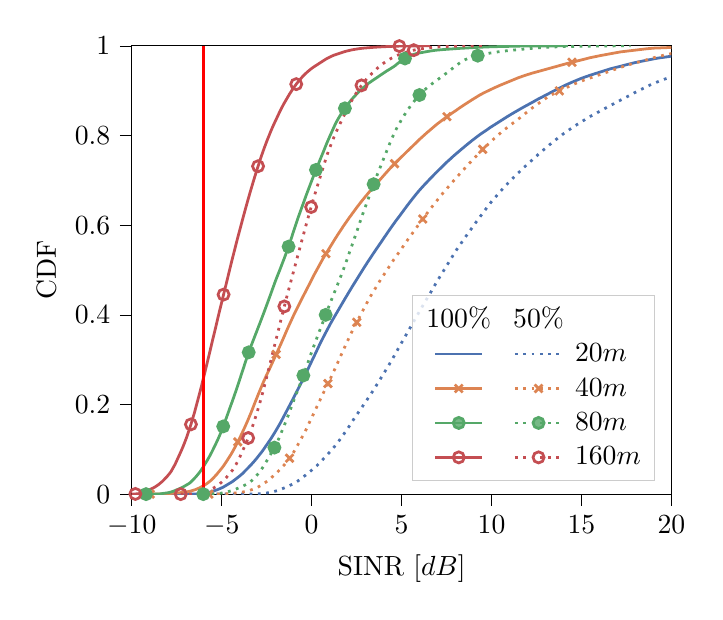
\begin{tikzpicture}

\definecolor{color0}{rgb}{0.298039215686275,0.447058823529412,0.690196078431373}
\definecolor{color1}{rgb}{0.866666666666667,0.517647058823529,0.32156862745098}
\definecolor{color2}{rgb}{0.333333333333333,0.658823529411765,0.407843137254902}
\definecolor{color3}{rgb}{0.768627450980392,0.305882352941176,0.32156862745098}

\begin{axis}[
legend cell align={left},
legend style={fill opacity=0.8, draw opacity=1, text opacity=1, draw=white!80!black},
legend columns=2,
legend style={
    font=\mystrut,
    legend cell align=left,
},
legend pos=south east,
tick align=outside,
tick pos=left,
x grid style={white!69.0196078431373!black},
xlabel={SINR [$dB$]},
xmin=-10, xmax=20,
xtick style={color=black},
y grid style={white!69.0196078431373!black},
ylabel={CDF},
ymin=0, ymax=1,
ytick style={color=black}
]
\addlegendimage{legend image with text=$100\%$}
\addlegendentry{}
% column 2 heading
\addlegendimage{legend image with text=$50\%$}
\addlegendentry{}
\addplot [line width=1pt, color0]
table {%
-8.2346830368042 2.86102294921875e-06
-6.47713613510132 0.000395894050598145
-6.33552694320679 0.000669360160827637
-6.17646741867065 0.00117921829223633
-6.03857183456421 0.00180304050445557
-5.91624593734741 0.0025094747543335
-5.82966089248657 0.00313043594360352
-5.78412294387817 0.00345516204833984
-5.70353698730469 0.00408470630645752
-5.65288972854614 0.00460028648376465
-5.59789133071899 0.00515007972717285
-5.25445938110352 0.00965356826782227
-5.23985052108765 0.00990986824035645
-5.16286277770996 0.0111575126647949
-4.92139196395874 0.0154217481613159
-4.41635751724243 0.0276331901550293
-4.32870626449585 0.0302252769470215
-4.29917907714844 0.031193733215332
-4.13757753372192 0.0361074209213257
-4.11883306503296 0.0366827249526978
-4.01309490203857 0.0399785041809082
-3.8983895778656 0.0439919233322144
-3.85989713668823 0.0452368259429932
-3.80981230735779 0.0471965074539185
-3.78745722770691 0.0481393337249756
-3.37279105186462 0.0651191473007202
-3.34583806991577 0.0662699937820435
-3.33494877815247 0.0667741298675537
-3.31126093864441 0.0679847002029419
-3.29568576812744 0.0686655044555664
-3.27981758117676 0.0693975687026978
-3.21857810020447 0.0720808506011963
-3.2077648639679 0.0726021528244019
-3.17432332038879 0.0741887092590332
-3.147620677948 0.0754221677780151
-3.08027195930481 0.0786153078079224
-2.7853581905365 0.0935128927230835
-2.77276563644409 0.0942078828811646
-2.76342153549194 0.0947177410125732
-2.74100613594055 0.0958999395370483
-2.69353985786438 0.0986201763153076
-2.67301416397095 0.0997453927993774
-2.65278673171997 0.100876212120056
-2.64188861846924 0.101497173309326
-2.25725245475769 0.124114155769348
-2.24367499351501 0.124971508979797
-2.03635883331299 0.138313770294189
-2.01388669013977 0.139820694923401
-1.93306910991669 0.145392298698425
-1.91165935993195 0.146862149238586
-1.8979777097702 0.147776484489441
-1.88135349750519 0.148850321769714
-1.84262979030609 0.151542186737061
-1.83148229122162 0.152302742004395
-1.78361284732819 0.15561830997467
-1.69557070732117 0.162018895149231
-1.68787670135498 0.162662625312805
-1.57876300811768 0.170954585075378
-1.5603084564209 0.172336101531982
-1.55044209957123 0.173076748847961
-1.51039361953735 0.176096081733704
-1.4697083234787 0.179141163825989
-1.45307397842407 0.180394411087036
-1.43960785865784 0.181511044502258
-1.42815852165222 0.182379841804504
-1.41473126411438 0.183351159095764
-1.39732921123505 0.184721350669861
-1.24597454071045 0.196271896362305
-1.23290085792542 0.197291612625122
-1.1558872461319 0.203233599662781
-1.1303882598877 0.20513641834259
-1.1135139465332 0.206463813781738
-1.08836364746094 0.208335280418396
-1.0699520111084 0.209768056869507
-1.05536687374115 0.210907459259033
-1.04592263698578 0.211682200431824
-1.01837456226349 0.213741660118103
-0.997763514518738 0.215447902679443
-0.988281965255737 0.216194152832031
-0.976494431495667 0.217054486274719
-0.952505946159363 0.218888878822327
-0.930152654647827 0.220657825469971
-0.914981126785278 0.221925377845764
-0.762786626815796 0.233794927597046
-0.731555342674255 0.236312985420227
-0.722948908805847 0.237013816833496
-0.668140649795532 0.241300702095032
-0.651078224182129 0.242645263671875
-0.642354488372803 0.243357300758362
-0.627087116241455 0.244627714157104
-0.539894819259644 0.251612186431885
-0.492215752601624 0.255694150924683
-0.481222629547119 0.256605625152588
-0.465227007865906 0.257930159568787
-0.456822991371155 0.258534073829651
-0.413414001464844 0.261966466903687
-0.342215657234192 0.267634987831116
-0.331525802612305 0.268498063087463
-0.325019359588623 0.269044995307922
-0.312063217163086 0.270113110542297
-0.302473664283752 0.270876526832581
-0.271637201309204 0.273408889770508
-0.265034079551697 0.273972868919373
-0.242783784866333 0.275798678398132
-0.225035071372986 0.277154564857483
-0.217900991439819 0.277744293212891
-0.148058652877808 0.283540964126587
-0.135816097259521 0.28465747833252
-0.122274041175842 0.285802602767944
-0.106503009796143 0.28713846206665
-0.095766544342041 0.288021564483643
-0.0703245401382446 0.290269017219543
-0.0372128486633301 0.292955160140991
-0.0250015258789062 0.294034719467163
0.0127769708633423 0.297327518463135
0.0348571538925171 0.29909360408783
0.0555497407913208 0.300740003585815
0.0682675838470459 0.301799654960632
0.23874843120575 0.316118955612183
0.254194498062134 0.317340970039368
0.260719537734985 0.317919254302979
0.268607378005981 0.318625688552856
0.328580617904663 0.323804140090942
0.356463432312012 0.326111435890198
0.377973914146423 0.327954411506653
0.422601222991943 0.331871151924133
0.48092257976532 0.336522698402405
0.53143835067749 0.340595960617065
0.569006681442261 0.343592643737793
0.586320281028748 0.344959855079651
0.612051367759705 0.347030758857727
0.660438537597656 0.350873351097107
1.01752316951752 0.378056406974792
1.03252792358398 0.379096150398254
1.08531033992767 0.383012771606445
1.13755762577057 0.386801242828369
1.15747356414795 0.38811731338501
1.18074369430542 0.389698147773743
1.73391771316528 0.427756786346436
1.77642226219177 0.430602431297302
1.79626548290253 0.431941151618958
1.81511580944061 0.433268547058105
1.82826614379883 0.434185743331909
1.87374365329742 0.437267780303955
1.88304150104523 0.437897324562073
1.89407968521118 0.438589572906494
1.9148428440094 0.440005302429199
1.95703446865082 0.442754030227661
1.98328626155853 0.444585561752319
2.04349517822266 0.448690295219421
2.05285429954529 0.449376821517944
2.07339572906494 0.450706958770752
2.10245370864868 0.452532887458801
2.11283183097839 0.453276395797729
2.14721846580505 0.455509543418884
2.17003226280212 0.456979393959045
2.18272709846497 0.457888007164001
2.19500327110291 0.458725452423096
2.21518087387085 0.460052847862244
2.23552989959717 0.461479902267456
2.25940656661987 0.463026642799377
2.26670551300049 0.463539361953735
2.2851870059967 0.464698791503906
2.2990345954895 0.465570449829102
2.93820905685425 0.506656885147095
2.95351052284241 0.507745027542114
2.97228026390076 0.508904337882996
3.01649498939514 0.511516332626343
3.03750205039978 0.512798309326172
3.05122876167297 0.513635635375977
3.07575988769531 0.51521372795105
3.08790469169617 0.51595151424408
3.0996458530426 0.51664936542511
3.12525701522827 0.518270254135132
3.18106651306152 0.521716833114624
3.18904948234558 0.522212505340576
3.19972205162048 0.522793531417847
3.22940230369568 0.524616599082947
3.28369760513306 0.527798414230347
3.35946321487427 0.532509803771973
3.38365268707275 0.533979535102844
3.41062140464783 0.535540580749512
3.43035054206848 0.536791086196899
3.4506847858429 0.537910461425781
3.48379135131836 0.539924383163452
3.50216197967529 0.54098105430603
3.5837824344635 0.545837879180908
3.63773488998413 0.548993945121765
3.69191575050354 0.55215859413147
3.70804595947266 0.553129911422729
3.71818113327026 0.5537109375
3.75392079353333 0.555816054344177
3.80408048629761 0.558781385421753
3.82166147232056 0.559744119644165
3.87200784683228 0.562709331512451
3.90200638771057 0.564401388168335
3.91523694992065 0.565170526504517
3.93888664245605 0.566606044769287
3.97160983085632 0.568662643432617
3.98373293876648 0.56942892074585
3.99818325042725 0.570289134979248
4.04488515853882 0.573040723800659
4.05436229705811 0.57361626625061
4.11958456039429 0.577399015426636
4.14381122589111 0.578803300857544
4.23145341873169 0.583947658538818
4.25507640838623 0.585371971130371
4.33991289138794 0.590222835540771
4.35690689086914 0.591214179992676
4.36913394927979 0.591954708099365
4.39101266860962 0.593108415603638
4.4021053314209 0.593769311904907
4.45551776885986 0.596925258636475
4.47411966323853 0.597905158996582
4.50973653793335 0.599896311759949
4.52102756500244 0.600505828857422
4.5478572845459 0.602009892463684
4.56491756439209 0.602946996688843
4.64002466201782 0.607174158096313
4.65654134750366 0.608148336410522
4.76651239395142 0.614024877548218
4.82036924362183 0.61688756942749
4.85834741592407 0.61887001991272
4.87775278091431 0.619892597198486
4.90328645706177 0.621191501617432
4.93540143966675 0.622946262359619
4.95074272155762 0.623880624771118
4.9781322479248 0.62535035610199
4.99271774291992 0.626190662384033
5.21411418914795 0.638202667236328
5.23289918899536 0.639162659645081
5.33385229110718 0.644762754440308
5.34611701965332 0.645312547683716
5.45641231536865 0.651146173477173
5.73326587677002 0.665229082107544
5.78732538223267 0.667886734008789
5.81997203826904 0.669570207595825
5.83616161346436 0.670307993888855
5.89003658294678 0.672877311706543
5.92684173583984 0.674688935279846
5.93910312652588 0.675250053405762
5.94975566864014 0.675779938697815
5.96488380432129 0.676503419876099
5.98458433151245 0.677380800247192
6.00521898269653 0.678332090377808
6.05049800872803 0.680309057235718
6.08282136917114 0.681824445724487
6.09497976303101 0.682394027709961
6.13136911392212 0.683977842330933
6.16052675247192 0.685288190841675
6.17476558685303 0.685877799987793
6.19923686981201 0.68693745136261
6.21005058288574 0.687453031539917
6.25528955459595 0.689415693283081
6.48892879486084 0.699288368225098
6.51421689987183 0.700342416763306
6.88383197784424 0.715766906738281
7.46440267562866 0.738611698150635
7.48072719573975 0.739204168319702
7.48966360092163 0.739571690559387
7.53065586090088 0.741178274154663
7.54541778564453 0.741705179214478
7.57319355010986 0.742744922637939
7.58965015411377 0.743317484855652
7.60633897781372 0.743915557861328
7.62360620498657 0.744542360305786
7.63715839385986 0.744978189468384
7.66852903366089 0.746120452880859
7.70708417892456 0.747481942176819
7.78959035873413 0.750566840171814
7.80436372756958 0.751119375228882
7.90504884719849 0.754828214645386
8.13353538513184 0.762661457061768
8.33094501495361 0.769352674484253
8.35814952850342 0.770349502563477
8.39689445495605 0.771580100059509
8.46582889556885 0.773836135864258
8.48962688446045 0.774739027023315
8.50398254394531 0.775214791297913
8.64520740509033 0.779909133911133
8.6974925994873 0.781492829322815
8.71299171447754 0.782005548477173
8.74100208282471 0.782999753952026
8.77001667022705 0.783925414085388
8.91211700439453 0.788548469543457
9.06067085266113 0.793023467063904
9.07773303985596 0.79361879825592
9.0896053314209 0.793994903564453
9.10875606536865 0.794558763504028
9.13704299926758 0.795453310012817
9.17813968658447 0.796752214431763
9.21863269805908 0.797914266586304
9.23400974273682 0.798418521881104
9.25568389892578 0.79905366897583
9.40373229980469 0.803429007530212
9.42925834655762 0.804109811782837
9.51919269561768 0.806499719619751
9.78890705108643 0.813834428787231
9.88125324249268 0.816560506820679
9.89774227142334 0.816993474960327
9.92999744415283 0.817939162254333
9.97196769714355 0.819015979766846
9.99399089813232 0.819554328918457
10.02796459198 0.82039737701416
10.0604104995728 0.821232080459595
10.0805187225342 0.821730494499207
10.8284358978271 0.840801119804382
10.852313041687 0.841419219970703
11.0940113067627 0.847358345985413
11.1270885467529 0.848135948181152
11.1420698165894 0.848517656326294
11.1788082122803 0.849332332611084
11.1881170272827 0.84958291053772
11.2093181610107 0.85004734992981
11.710991859436 0.861694812774658
11.7362537384033 0.862224578857422
11.7835178375244 0.863284111022949
11.7984237670898 0.863620281219482
11.8205194473267 0.864118814468384
11.839674949646 0.864551782608032
11.8649711608887 0.865095853805542
11.8908138275146 0.865656971931458
11.9111642837524 0.866109848022461
12.2460289001465 0.873399138450623
12.2843399047852 0.874290704727173
12.3239774703979 0.875162363052368
12.4595146179199 0.878224492073059
12.4806461334229 0.878734350204468
12.5195817947388 0.879585981369019
12.6074628829956 0.88152015209198
12.6546401977539 0.882517099380493
12.7227773666382 0.883867263793945
12.7789936065674 0.885026693344116
12.8378324508667 0.886200189590454
12.8627452850342 0.886764287948608
12.9179344177246 0.887946367263794
12.9651746749878 0.888968944549561
13.1168775558472 0.892082333564758
13.4181900024414 0.89847719669342
13.4430961608887 0.899041175842285
13.9094047546387 0.908395648002625
13.9393606185913 0.908962488174438
14.0426950454712 0.910967826843262
14.0711765289307 0.911491870880127
14.1448926925659 0.912890553474426
14.3220453262329 0.916083693504333
14.3563394546509 0.916721820831299
14.4221878051758 0.917841196060181
14.4614124298096 0.918539047241211
14.7282295227051 0.923062443733215
14.8767347335815 0.925497889518738
14.9129619598389 0.926121711730957
14.9270362854004 0.926346778869629
14.9637069702148 0.926953554153442
15.0241661071777 0.927819490432739
15.0924272537231 0.92886483669281
15.1685123443604 0.930041313171387
15.2059984207153 0.930576801300049
15.2937602996826 0.931710481643677
15.3368673324585 0.932297229766846
15.4459571838379 0.933946490287781
15.5082426071167 0.934721231460571
16.6050109863281 0.948624730110168
16.6286010742188 0.948878288269043
16.7040882110596 0.949684381484985
16.8437767028809 0.951114416122437
16.8879909515381 0.95160710811615
16.9982395172119 0.95265531539917
17.0669326782227 0.953304767608643
17.1370906829834 0.953982830047607
17.3303508758545 0.956076383590698
17.3789978027344 0.95665454864502
17.431432723999 0.957190155982971
17.9476280212402 0.962283253669739
18.0129318237305 0.962850093841553
18.1618099212646 0.96402645111084
18.1879463195801 0.964265823364258
18.2629127502441 0.964900970458984
18.3689308166504 0.965781211853027
18.4582805633545 0.966504693031311
18.5479431152344 0.967191219329834
19.1396045684814 0.971780061721802
19.2523784637451 0.97256338596344
19.3112010955811 0.97291088104248
20.8129348754883 0.981473445892334
20.905689239502 0.981917858123779
21.0511474609375 0.982621431350708
21.1911811828613 0.983219623565674
22.1478900909424 0.987042188644409
22.3168525695801 0.987623333930969
22.5631313323975 0.988492131233215
22.7138786315918 0.98897922039032
22.8514499664307 0.989457845687866
23.139404296875 0.990508794784546
23.2235851287842 0.990847826004028
23.3376445770264 0.99134635925293
23.7183971405029 0.99285888671875
23.7746276855469 0.993035435676575
23.9640979766846 0.993727684020996
24.344274520874 0.995100617408752
24.3927040100098 0.995297193527222
24.6590118408203 0.995835542678833
24.7271709442139 0.995995044708252
25.5141754150391 0.997413635253906
26.0013694763184 0.998404860496521
27.8405475616455 0.999717950820923
31.5434246063232 0.999985694885254
37.7558517456055 1
};
\addlegendentry{}
\addplot [line width=1pt, color0, dotted]
table {%
-5.29767847061157 2.86102294921875e-06
-3.21054434776306 0.000393033027648926
-2.86758661270142 0.0010141134262085
-2.31903910636902 0.00346660614013672
-1.89734649658203 0.00795292854309082
-1.59118664264679 0.01276695728302
-1.56257128715515 0.0132226943969727
-1.52730309963226 0.0138123035430908
-1.22151374816895 0.0192699432373047
-1.19115340709686 0.019853949546814
-1.1239265203476 0.0211784839630127
-1.0118602514267 0.0234915018081665
-0.916948795318604 0.0256278514862061
-0.896071195602417 0.0261291265487671
-0.856247305870056 0.02704918384552
-0.812741041183472 0.0281715393066406
-0.793360233306885 0.0286756753921509
-0.726599216461182 0.0304673910140991
-0.677252054214478 0.0318688154220581
-0.666764140129089 0.0321906805038452
-0.653422594070435 0.0326550006866455
-0.613309741020203 0.0339169502258301
-0.599470257759094 0.0343641042709351
-0.560222864151001 0.035617470741272
-0.522716522216797 0.0367368459701538
-0.498233318328857 0.0374945402145386
-0.485976219177246 0.037873387336731
-0.467987298965454 0.0384231805801392
-0.327236413955688 0.0425820350646973
-0.272487640380859 0.0443707704544067
-0.247012257575989 0.0450800657272339
-0.195846199989319 0.0467407703399658
-0.165422916412354 0.0477291345596313
-0.0538008213043213 0.051594614982605
0.317118644714355 0.0645437240600586
0.461777329444885 0.070428729057312
0.530511140823364 0.0732601881027222
0.553762674331665 0.0742229223251343
0.610532999038696 0.0767865180969238
0.62342357635498 0.0773391723632812
0.66102409362793 0.0790824890136719
0.675588130950928 0.07967209815979
0.707980394363403 0.0810136795043945
0.790048599243164 0.0844318866729736
0.809442758560181 0.0853490829467773
0.830447196960449 0.0862008333206177
0.869110226631165 0.0877219438552856
0.897032976150513 0.0889126062393188
0.934733510017395 0.0906729698181152
0.963579654693604 0.0919604301452637
1.00589299201965 0.0938718318939209
1.02056705951691 0.0945127010345459
1.07666385173798 0.0969452857971191
1.11520254611969 0.0986629724502563
1.12669837474823 0.0991699695587158
1.14856839179993 0.100126981735229
1.17804455757141 0.101619601249695
1.20830738544464 0.103086590766907
1.23886930942535 0.104613423347473
1.34362006187439 0.109649538993835
1.39261627197266 0.112253069877625
1.44621515274048 0.115073084831238
1.46193075180054 0.115856409072876
1.49855589866638 0.117810487747192
1.50877439975739 0.118345975875854
1.51976907253265 0.118972659111023
1.5616147518158 0.121109008789062
1.79418742656708 0.13431453704834
1.82941997051239 0.136251449584961
1.84879672527313 0.137271285057068
1.87049829959869 0.138439178466797
1.89900529384613 0.140102624893188
1.92094528675079 0.141430020332336
1.9440301656723 0.142686247825623
1.9595890045166 0.143592000007629
1.98562145233154 0.145172953605652
2.07282161712646 0.150516748428345
2.08368325233459 0.15119469165802
2.11586356163025 0.153194308280945
2.13390612602234 0.154233932495117
2.19979310035706 0.158483982086182
2.25019383430481 0.161543130874634
2.26316118240356 0.162349343299866
2.37276935577393 0.169174313545227
2.38921427726746 0.170159816741943
2.50883674621582 0.177167177200317
2.52027130126953 0.177887797355652
2.53721952438354 0.178790807723999
2.55401039123535 0.179779171943665
2.57075452804565 0.180756211280823
2.60657429695129 0.18290114402771
2.61616206169128 0.183496475219727
2.62532734870911 0.18406617641449
2.64151215553284 0.18499755859375
2.65320038795471 0.185627102851868
2.7009437084198 0.188318967819214
2.71735143661499 0.189313054084778
2.73366117477417 0.19035279750824
2.76773643493652 0.192261219024658
2.91545248031616 0.200610160827637
3.38106489181519 0.228644967079163
3.40491557121277 0.230080604553223
3.42576599121094 0.231316804885864
3.46693778038025 0.234005808830261
3.52056097984314 0.237301468849182
4.1825737953186 0.280475854873657
4.19931602478027 0.281595349311829
4.21834945678711 0.282939910888672
4.27858304977417 0.287053108215332
4.32230710983276 0.289861679077148
4.34260559082031 0.291191935539246
4.35875701904297 0.292453765869141
4.3800745010376 0.293966293334961
4.39399147033691 0.294923424720764
4.40657472610474 0.295843482017517
4.41742467880249 0.296464443206787
4.52665233612061 0.304018616676331
4.55554008483887 0.3059983253479
4.57716941833496 0.307530879974365
4.59283208847046 0.308681607246399
4.60843229293823 0.309923529624939
4.6186637878418 0.310595750808716
4.62794256210327 0.311310768127441
4.63780736923218 0.311980128288269
4.67571973800659 0.314757466316223
4.8273868560791 0.325527548789978
4.83955430984497 0.326316595077515
4.87980365753174 0.329093813896179
4.88689136505127 0.329592347145081
4.90711498260498 0.330985307693481
4.92965221405029 0.33262026309967
4.95672941207886 0.33463978767395
4.97897005081177 0.33615517616272
4.98927783966064 0.336901545524597
5.01019859313965 0.338379859924316
5.26526212692261 0.356276988983154
5.2916111946106 0.358105659484863
5.30628633499146 0.359074115753174
5.3281192779541 0.360580921173096
5.33624505996704 0.361199140548706
5.34937906265259 0.362082123756409
5.64849233627319 0.383289098739624
5.72613191604614 0.388746738433838
5.74976062774658 0.39044451713562
5.81459617614746 0.394976377487183
5.82771682739258 0.395939230918884
6.15311002731323 0.418559074401855
6.22641134262085 0.423566579818726
6.23466491699219 0.424173355102539
6.26109266281128 0.425965070724487
6.28001117706299 0.427212715148926
6.2949423789978 0.428238153457642
6.32049703598022 0.430027008056641
6.35679006576538 0.432539343833923
6.41359710693359 0.436475992202759
6.4333324432373 0.437891721725464
6.49411392211914 0.442104578018188
6.50039577484131 0.442523241043091
6.54817485809326 0.445548415184021
6.61787509918213 0.450051784515381
6.63112926483154 0.450994729995728
6.71321058273315 0.456896781921387
6.72282791137695 0.457540512084961
6.7402777671814 0.458657145500183
6.75209093093872 0.459537267684937
6.76496982574463 0.460346221923828
6.77980279922485 0.46138596534729
6.79641342163086 0.462553858757019
6.8586859703064 0.466855049133301
6.93208265304565 0.471822738647461
6.95818471908569 0.473506212234497
7.04132604598999 0.479220271110535
7.05268955230713 0.479938149452209
7.07242250442505 0.481202840805054
7.09990692138672 0.482991695404053
8.00678157806396 0.541986703872681
8.01607131958008 0.542536377906799
8.04908657073975 0.544567346572876
8.06827735900879 0.545812129974365
8.07951736450195 0.546404600143433
8.11101818084717 0.548136472702026
8.14987850189209 0.550492286682129
8.16404056549072 0.55138373374939
8.21248626708984 0.554246544837952
8.33277988433838 0.561037302017212
8.36660766601562 0.563034057617188
8.37568664550781 0.563595294952393
8.38712310791016 0.564275979995728
8.40593242645264 0.565415382385254
8.42245101928711 0.566375374794006
8.4377555847168 0.56725549697876
8.63910579681396 0.578603982925415
8.65025901794434 0.579310297966003
8.72573947906494 0.583346605300903
8.75350475311279 0.584896206855774
8.78309154510498 0.586588144302368
9.072190284729 0.602656483650208
9.11410999298096 0.60505199432373
9.12099361419678 0.605502128601074
9.15878200531006 0.607561588287354
9.16923332214355 0.608128428459167
9.18768501281738 0.609059810638428
9.21854496002197 0.610754728317261
9.22781372070312 0.611267447471619
9.24044036865234 0.611968159675598
9.34785842895508 0.617944240570068
9.37404346466064 0.619379997253418
9.38798522949219 0.62011194229126
9.40893840789795 0.62115740776062
9.46725177764893 0.624404668807983
9.51216125488281 0.626897096633911
9.54117774963379 0.628401041030884
9.56036186218262 0.629492044448853
9.61299896240234 0.632269382476807
9.62770557403564 0.633009910583496
9.65037536621094 0.634200572967529
9.69150543212891 0.636399626731873
9.73315048217773 0.63865852355957
9.74264049530029 0.639156937599182
9.85776996612549 0.645155906677246
9.86896896362305 0.645736932754517
9.89625072479248 0.647127032279968
9.93505382537842 0.649206399917603
9.94313526153564 0.649656534194946
9.96574115753174 0.65080726146698
10.0698328018188 0.655780792236328
10.1239538192749 0.658321619033813
10.2466764450073 0.663907408714294
10.2636375427246 0.664667963981628
10.288254737854 0.665784597396851
10.3061227798462 0.666627764701843
10.3488922119141 0.668587446212769
10.4675874710083 0.674136400222778
10.4821453094482 0.6747145652771
10.509033203125 0.675908088684082
10.5184564590454 0.676332473754883
10.5373334884644 0.677184224128723
10.55286693573 0.677890658378601
10.5764474868774 0.679032802581787
10.596960067749 0.679987192153931
10.6091384887695 0.68053126335144
10.6557235717773 0.682582139968872
10.6923723220825 0.684174418449402
10.97265625 0.69594144821167
10.9848251342773 0.696394443511963
11.2209091186523 0.706102013587952
11.2453594207764 0.70719575881958
11.2785530090332 0.708420753479004
11.301851272583 0.709317922592163
11.3188419342041 0.710072755813599
11.3635339736938 0.71177339553833
11.4269504547119 0.714223027229309
11.4534273147583 0.715177297592163
11.808424949646 0.728944063186646
11.8213386535645 0.729396939277649
11.990086555481 0.735700607299805
12.0024509429932 0.736162066459656
12.0518283843994 0.737953782081604
12.1093282699585 0.740050315856934
12.1250782012939 0.740523099899292
12.1401338577271 0.741021633148193
12.1620769500732 0.741833448410034
12.18505859375 0.742679357528687
12.2136564254761 0.743770360946655
12.3069877624512 0.747140169143677
12.3608093261719 0.74902868270874
12.3921661376953 0.750187993049622
12.4130382537842 0.750948548316956
12.4254341125488 0.751389980316162
12.4692211151123 0.752962350845337
12.5110654830933 0.754486322402954
12.5242309570312 0.755016207695007
12.586181640625 0.757337689399719
12.6100673675537 0.758195161819458
12.9053993225098 0.768347024917603
12.9383678436279 0.769435167312622
12.9544811248779 0.76998496055603
12.9689502716064 0.770454883575439
12.9890184402466 0.771161317825317
13.2180957794189 0.778986215591431
13.2419424057007 0.779874920845032
13.3084735870361 0.781982779502869
13.3279066085815 0.782592296600342
13.5635356903076 0.790306091308594
13.6676139831543 0.793576121330261
13.6839389801025 0.794117331504822
13.7379188537598 0.795760869979858
13.8362579345703 0.798803091049194
13.8519926071167 0.79928731918335
13.9175052642822 0.801261305809021
13.9434986114502 0.802132964134216
13.9661884307861 0.802847862243652
14.003098487854 0.803916096687317
14.5947208404541 0.820360422134399
14.6148386001587 0.820841789245605
14.9282312393188 0.828814744949341
14.9542102813721 0.829404354095459
15.3636541366577 0.839581966400146
15.3824338912964 0.840051889419556
15.5182161331177 0.843159675598145
15.5753326416016 0.844424366950989
15.6016292572021 0.845011234283447
15.6729602813721 0.846455335617065
15.6862325668335 0.846725940704346
15.7065238952637 0.847187399864197
15.9134492874146 0.851725101470947
15.9429569244385 0.852343082427979
15.9623937606812 0.852804660797119
16.0447635650635 0.854676008224487
16.1883506774902 0.857698321342468
16.3059940338135 0.86033034324646
16.3295803070068 0.860794544219971
16.3563804626465 0.861324429512024
16.4096164703369 0.862509489059448
16.5790157318115 0.866098403930664
16.634557723999 0.867363214492798
16.6571655273438 0.8678218126297
17.1606483459473 0.878574848175049
17.1848812103271 0.879070520401001
17.3322086334229 0.882041454315186
17.344030380249 0.882349014282227
17.3754062652588 0.882952928543091
17.6795272827148 0.889401912689209
17.6956157684326 0.889803647994995
17.7186164855957 0.890344858169556
17.7556896209717 0.891099691390991
17.779411315918 0.891578197479248
17.876558303833 0.89370322227478
17.8986968994141 0.894232988357544
17.930082321167 0.894942283630371
18.0799007415771 0.897961616516113
18.1223125457764 0.898753523826599
18.226806640625 0.900869846343994
18.2798042297363 0.90204918384552
18.5823516845703 0.907800316810608
18.6742820739746 0.909685969352722
18.707181930542 0.910304069519043
18.8176708221436 0.91264271736145
18.8493099212646 0.913232326507568
18.9255275726318 0.914608240127563
19.442476272583 0.92304539680481
19.6118717193604 0.925466537475586
19.949857711792 0.930081129074097
19.9820499420166 0.930528402328491
20.0416984558105 0.931308746337891
20.0643405914307 0.931607961654663
20.0983028411865 0.932038068771362
20.2690563201904 0.934345245361328
20.3237705230713 0.935063123703003
20.3756980895996 0.935718297958374
20.4716625213623 0.936843395233154
20.4978733062744 0.93721079826355
20.6678905487061 0.939327239990234
20.7137546539307 0.939834356307983
20.7344360351562 0.940030813217163
20.7803173065186 0.940549373626709
20.8212203979492 0.94101357460022
20.8715038299561 0.941614627838135
20.9224166870117 0.942195653915405
20.9784660339355 0.942862272262573
21.0439224243164 0.943588614463806
21.1207218170166 0.944440364837646
21.1651058197021 0.944881916046143
21.2176570892334 0.945485711097717
22.9579887390137 0.963359951972961
23.0525798797607 0.96406352519989
23.0671977996826 0.964185953140259
23.3601398468018 0.966382265090942
23.4316539764404 0.966883540153503
23.5200977325439 0.967524528503418
23.7375583648682 0.969074010848999
24.0882759094238 0.971600532531738
24.2599315643311 0.972785592079163
24.3750705718994 0.973517656326294
24.451961517334 0.974016189575195
24.7573146820068 0.975919008255005
24.8649291992188 0.976534128189087
24.988000869751 0.977197885513306
25.2166957855225 0.978488206863403
25.3219757080078 0.979049444198608
25.3682880401611 0.979285836219788
25.5559177398682 0.980297088623047
25.6721954345703 0.980926513671875
25.7198963165283 0.981174349784851
28.3581352233887 0.993009805679321
30.3601760864258 0.99685525894165
31.1142501831055 0.997692704200745
31.3163433074951 0.997912049293518
32.5096015930176 0.99891185760498
32.6625633239746 0.99898886680603
36.4671058654785 0.999837636947632
42.4160308837891 0.999982833862305
46.6679344177246 1
};
\addlegendentry{$20m$}

\addplot [line width=1pt, color1, mark=x, mark repeat={50}]
table {%
-8.97454357147217 2.74181365966797e-06
-8.17666721343994 0.000431060791015625
-7.16145658493042 0.00376284122467041
-7.11750507354736 0.00402152538299561
-7.03772878646851 0.00448048114776611
-6.81371259689331 0.00614082813262939
-6.7483286857605 0.00667202472686768
-6.68556451797485 0.00728380680084229
-6.47970962524414 0.00989532470703125
-6.46336650848389 0.0101456642150879
-6.43146896362305 0.0105767250061035
-6.21035623550415 0.0145008563995361
-6.17642736434937 0.0152490139007568
-6.04446315765381 0.0180552005767822
-6.02393913269043 0.0185223817825317
-5.93163347244263 0.0207529067993164
-5.86441850662231 0.0224326848983765
-5.72661638259888 0.0264875888824463
-5.66613912582397 0.0283955335617065
-5.64677333831787 0.0289851427078247
-5.62718057632446 0.029666543006897
-5.61213493347168 0.0302032232284546
-5.58494281768799 0.0311433076858521
-5.48220682144165 0.0350563526153564
-5.41739845275879 0.0379320383071899
-5.40346050262451 0.0385717153549194
-5.34486103057861 0.0412166118621826
-5.319899559021 0.0422928333282471
-5.2668662071228 0.0446068048477173
-5.25431060791016 0.0451490879058838
-5.20815944671631 0.0474991798400879
-5.19700622558594 0.0480610132217407
-5.17316722869873 0.0491762161254883
-4.99460697174072 0.0579173564910889
-4.98214340209961 0.0586071014404297
-4.93700504302979 0.0609849691390991
-4.92079591751099 0.0618360042572021
-4.90470457077026 0.0626730918884277
-4.86098146438599 0.0652456283569336
-4.84322595596313 0.0661383867263794
-4.83109760284424 0.0669533014297485
-4.80064630508423 0.0687805414199829
-4.78871870040894 0.0695704221725464
-4.76620435714722 0.0707941055297852
-4.73749589920044 0.0725656747817993
-4.48700618743896 0.0884182453155518
-4.44968032836914 0.0909240245819092
-4.25646257400513 0.104835271835327
-4.15624952316284 0.112756013870239
-4.13455057144165 0.114391326904297
-4.10611629486084 0.116541147232056
-4.08297395706177 0.118412852287292
-4.06749773025513 0.119455814361572
-4.04466962814331 0.121283054351807
-4.03400039672852 0.122167348861694
-4.02662181854248 0.122807025909424
-3.99204730987549 0.125679969787598
-3.97447419166565 0.127001047134399
-3.93753695487976 0.13029944896698
-3.91671323776245 0.132171154022217
-3.90294003486633 0.133394837379456
-3.88873052597046 0.134588003158569
-3.86477184295654 0.136590480804443
-3.85442280769348 0.137413620948792
-3.80333876609802 0.141805052757263
-3.7797474861145 0.143693447113037
-3.67339062690735 0.153065919876099
-3.58528733253479 0.161020040512085
-3.41605424880981 0.177211880683899
-3.38805675506592 0.179815053939819
-3.37941312789917 0.180674314498901
-3.32099413871765 0.186634302139282
-3.30563807487488 0.188216805458069
-3.26242613792419 0.192569375038147
-3.1977903842926 0.199274659156799
-3.18282914161682 0.200843214988708
-3.15304231643677 0.203966498374939
-2.92743849754333 0.22637140750885
-2.90799164772034 0.228223562240601
-2.85993242263794 0.232729077339172
-2.84444093704224 0.234244823455811
-2.83332276344299 0.235343337059021
-2.781081199646 0.240427255630493
-2.76976346969604 0.241472959518433
-2.73741006851196 0.244637966156006
-2.72152829170227 0.246156454086304
-2.70736837387085 0.247485876083374
-2.69505429267883 0.248637199401855
-2.68039226531982 0.250044465065002
-2.67383527755737 0.250603437423706
-2.60365867614746 0.256822109222412
-2.5328164100647 0.263229846954346
-2.5123975276947 0.264979243278503
-2.45417857170105 0.269899129867554
-2.42938804626465 0.271932125091553
-2.41803693771362 0.272919416427612
-2.32608723640442 0.280653834342957
-2.31693744659424 0.281429767608643
-2.01003623008728 0.30837345123291
-1.99179577827454 0.310019969940186
-1.97386002540588 0.311658024787903
-1.93262684345245 0.315287351608276
-1.91714179515839 0.31665301322937
-1.76966714859009 0.329715967178345
-1.76022958755493 0.330533623695374
-1.72214663028717 0.333929419517517
-1.58305251598358 0.346586465835571
-1.57285964488983 0.347479104995728
-1.55767059326172 0.348925352096558
-1.44804060459137 0.359132170677185
-1.44053995609283 0.35985803604126
-1.43265271186829 0.360575556755066
-1.42447650432587 0.361334800720215
-1.4122496843338 0.362505674362183
-1.39988136291504 0.363582015037537
-1.36680054664612 0.366621732711792
-1.33575916290283 0.369402885437012
-1.32221436500549 0.370707273483276
-1.30597531795502 0.372072815895081
-1.291539311409 0.373371601104736
-1.1745001077652 0.383686900138855
-1.15055334568024 0.385703206062317
-1.12543284893036 0.387964248657227
-1.03279042243958 0.396140813827515
-1.02322232723236 0.396939039230347
-1.01506066322327 0.397656679153442
-0.966125726699829 0.401922941207886
-0.950842142105103 0.403149366378784
-0.875200510025024 0.409281730651855
-0.864407420158386 0.410188436508179
-0.804135322570801 0.415024876594543
-0.780034899711609 0.416910409927368
-0.763006210327148 0.418251037597656
-0.74157452583313 0.419983625411987
-0.672568559646606 0.425281763076782
-0.651890635490417 0.426964282989502
-0.522687673568726 0.437432527542114
-0.41750955581665 0.445603609085083
-0.099429726600647 0.470369696617126
-0.0346146821975708 0.475514769554138
-0.0254251956939697 0.476193428039551
-0.00154709815979004 0.477970600128174
0.0133864879608154 0.479238748550415
0.0202492475509644 0.479728221893311
0.0278716087341309 0.4803706407547
0.0958520174026489 0.485830068588257
0.106059551239014 0.486650466918945
0.159751534461975 0.490855574607849
0.622334957122803 0.524713277816772
0.784016132354736 0.535465240478516
0.795635461807251 0.536266088485718
0.825116634368896 0.538204669952393
0.987116575241089 0.548697948455811
1.00782310962677 0.549996614456177
1.02667224407196 0.55125093460083
1.03851556777954 0.552043557167053
1.06579542160034 0.553792953491211
1.09972870349884 0.556109666824341
1.16777741909027 0.560489892959595
1.33220374584198 0.571294665336609
1.3711793422699 0.573694825172424
1.46117913722992 0.579201459884644
1.49858629703522 0.581448554992676
1.66072797775269 0.591291189193726
1.71440970897675 0.594672918319702
1.74128329753876 0.596313953399658
1.77319729328156 0.598305225372314
1.94124448299408 0.60794734954834
1.96233224868774 0.609173893928528
1.9858912229538 0.610472679138184
2.00494456291199 0.611613035202026
2.01275730133057 0.612010717391968
2.0240912437439 0.61263632774353
2.0438666343689 0.613776683807373
2.05688881874084 0.614496946334839
2.08681106567383 0.616293668746948
2.11288189888 0.617809295654297
2.15716552734375 0.620126008987427
2.18754649162292 0.621705770492554
2.27116632461548 0.62647819519043
2.28904175758362 0.627376556396484
2.52989315986633 0.640534162521362
2.54106330871582 0.6411292552948
2.60503602027893 0.64437198638916
2.71010661125183 0.649973273277283
2.97166442871094 0.662897348403931
3.0071702003479 0.664616107940674
3.06410312652588 0.667333126068115
3.0828070640564 0.668245434761047
3.11406707763672 0.669755578041077
3.15110921859741 0.671610593795776
3.16391944885254 0.672147393226624
3.17610931396484 0.672728657722473
4.10296678543091 0.715102195739746
4.16529273986816 0.717816591262817
4.20660257339478 0.719691038131714
4.24066734313965 0.721226215362549
4.31067562103271 0.724388360977173
4.31681632995605 0.724711060523987
4.57448434829712 0.735621452331543
4.60999011993408 0.736950874328613
4.63149166107178 0.737743496894836
4.7032470703125 0.740622043609619
4.72987413406372 0.741676092147827
5.06771278381348 0.754975557327271
5.20614290237427 0.760418176651001
5.22871923446655 0.761347055435181
5.31377267837524 0.764676094055176
5.33032369613647 0.765362977981567
5.36053419113159 0.766481041908264
5.38044786453247 0.767154097557068
5.72053909301758 0.780439615249634
5.73696660995483 0.781001448631287
5.76108264923096 0.781994342803955
5.77141046524048 0.782389163970947
5.90645551681519 0.787606716156006
5.97825241088867 0.790532350540161
5.99413537979126 0.791080236434937
6.00868463516235 0.791669845581055
6.05733871459961 0.793452620506287
6.15042209625244 0.796817779541016
6.1698751449585 0.797532558441162
6.19225931167603 0.798397541046143
6.21394491195679 0.799142837524414
6.24380350112915 0.800216436386108
6.2670750617981 0.801125764846802
6.3115234375 0.802741646766663
6.34966564178467 0.804054379463196
6.36334848403931 0.804582834243774
6.38922166824341 0.805514454841614
6.62008905410767 0.813374042510986
6.70258474349976 0.816202402114868
6.71682548522949 0.816728115081787
6.74087047576904 0.817556858062744
6.83467054367065 0.820735692977905
6.86416435241699 0.821756362915039
6.88381242752075 0.822482228279114
6.91970777511597 0.823625326156616
7.0033712387085 0.82632577419281
7.03306722640991 0.827235221862793
7.06524515151978 0.828230857849121
7.12518692016602 0.830038547515869
7.15772390365601 0.831003665924072
7.18404960632324 0.831810235977173
7.21854496002197 0.832903146743774
7.3374981880188 0.836412906646729
7.43170595169067 0.839099645614624
7.44552230834961 0.839541792869568
7.49361276626587 0.841010212898254
7.50445652008057 0.841393947601318
7.52197408676147 0.841883420944214
7.5498046875 0.842681646347046
7.57036542892456 0.84323787689209
7.79990577697754 0.849743008613586
7.81737661361694 0.850196361541748
7.85643625259399 0.85128927230835
7.91313886642456 0.852796792984009
7.9661693572998 0.854173421859741
7.98350524902344 0.854635000228882
8.02028179168701 0.855602979660034
8.15509700775146 0.859546542167664
8.27180194854736 0.862772703170776
8.29626083374023 0.8633873462677
8.35228157043457 0.864986419677734
8.38036918640137 0.865731835365295
8.85315227508545 0.877968788146973
8.87000942230225 0.878411054611206
8.91521549224854 0.879570841789246
9.31906318664551 0.88956356048584
9.35554313659668 0.890383958816528
9.39337253570557 0.891190528869629
9.41736030578613 0.89170503616333
9.49843978881836 0.893490433692932
9.55036354064941 0.894633531570435
9.6452054977417 0.896432876586914
9.69126605987549 0.897364616394043
9.7471170425415 0.898463129997253
9.95211219787598 0.902395725250244
10.122332572937 0.905674695968628
10.1865453720093 0.906848311424255
10.2147693634033 0.907365560531616
10.2331113815308 0.907702088356018
10.248607635498 0.907944083213806
10.3245010375977 0.909229040145874
10.4126167297363 0.910822629928589
10.4951829910278 0.912313222885132
11.4689197540283 0.92842161655426
11.4991912841797 0.928880453109741
11.5359563827515 0.929439544677734
11.583065032959 0.930062532424927
11.6886205673218 0.931597709655762
12.033052444458 0.93618381023407
12.0753326416016 0.936712265014648
12.1709003448486 0.93797492980957
12.2281408309937 0.93867301940918
14.2240600585938 0.960835933685303
14.2754917144775 0.961339235305786
14.3269805908203 0.961842656135559
14.3886137008667 0.962440609931946
14.4131736755371 0.962721586227417
14.4736557006836 0.963297128677368
14.497181892395 0.963519692420959
14.556827545166 0.964103698730469
15.2418737411499 0.970937013626099
15.2800607681274 0.971384763717651
15.358528137207 0.972224712371826
15.4083223342896 0.97278368473053
15.440824508667 0.973098039627075
15.6341991424561 0.974772214889526
15.7010622024536 0.975317239761353
15.8395042419434 0.976413011550903
16.0311832427979 0.978054046630859
17.1593170166016 0.986369609832764
18.5672550201416 0.993102788925171
18.6875343322754 0.993606090545654
18.9694042205811 0.994632363319397
19.0283718109131 0.994827032089233
21.7763061523438 0.999082207679749
24.7004451751709 0.999799728393555
28.8756313323975 1
};
\addlegendentry{}
\addplot [line width=1pt, color1,dotted, mark=x, mark repeat={50}, mark options={solid}]
table {%
-5.71035194396973 2.74181365966797e-06
-4.91172552108765 0.000453352928161621
-4.65253782272339 0.00106239318847656
-4.5830979347229 0.00128209590911865
-4.39105749130249 0.0019690990447998
-4.33789873123169 0.00218319892883301
-3.97503709793091 0.00390756130218506
-3.93009328842163 0.00415229797363281
-3.84419989585876 0.00463616847991943
-3.8191978931427 0.00478363037109375
-3.62939715385437 0.00608515739440918
-3.58735966682434 0.00641334056854248
-3.52290487289429 0.00709474086761475
-3.12185311317444 0.0129601955413818
-2.97156643867493 0.0159637928009033
-2.93204236030579 0.0168648958206177
-2.8894145488739 0.0178772211074829
-2.86421823501587 0.0184084177017212
-2.83057641983032 0.0191870927810669
-2.77456545829773 0.0206166505813599
-2.74815511703491 0.0212507247924805
-2.61147236824036 0.024977445602417
-2.53269410133362 0.0271635055541992
-2.42981290817261 0.0302226543426514
-2.41553330421448 0.0306955575942993
-2.37278032302856 0.032008171081543
-2.35341835021973 0.0325922966003418
-2.33475208282471 0.0331095457077026
-2.31212449073792 0.0338548421859741
-1.95425593852997 0.047132134437561
-1.92835342884064 0.0481499433517456
-1.87765157222748 0.0501914024353027
-1.82137322425842 0.0524774789810181
-1.76154828071594 0.0549108982086182
-1.74631607532501 0.055600643157959
-1.7358785867691 0.0560456514358521
-1.68599081039429 0.0579924583435059
-1.62962400913239 0.0604064464569092
-1.61721920967102 0.0609849691390991
-1.54998910427094 0.0640414953231812
-1.51012909412384 0.0658631324768066
-1.4732518196106 0.0675373077392578
-1.4354385137558 0.0693395137786865
-1.41900873184204 0.070076584815979
-1.354079246521 0.0733749866485596
-1.33701395988464 0.0742510557174683
-1.31941068172455 0.0751187801361084
-1.28671872615814 0.0767290592193604
-1.26888823509216 0.0777413845062256
-1.24578928947449 0.0791208744049072
-1.22715449333191 0.0802360773086548
-1.19569230079651 0.0819882154464722
-1.13338279724121 0.0855202674865723
-1.11105048656464 0.0868607759475708
-1.02170372009277 0.0922117233276367
-0.984906196594238 0.094678521156311
-0.914746403694153 0.099570631980896
-0.892519235610962 0.101175308227539
-0.868661642074585 0.102699398994446
-0.813767194747925 0.106490135192871
-0.791340231895447 0.108144879341125
-0.77259635925293 0.10950767993927
-0.706103682518005 0.114399671554565
-0.6716548204422 0.116925001144409
-0.657821655273438 0.1179039478302
-0.645196437835693 0.118807792663574
-0.617928385734558 0.120813012123108
-0.605159044265747 0.121702909469604
-0.596590518951416 0.12236487865448
-0.588080406188965 0.12300169467926
-0.435191631317139 0.134148597717285
-0.410289764404297 0.135953545570374
-0.298665642738342 0.14483654499054
-0.232688069343567 0.150440573692322
-0.206576824188232 0.152848958969116
-0.194237232208252 0.153858542442322
-0.0911067724227905 0.162666440010071
0.0227402448654175 0.172239184379578
0.0407896041870117 0.173690915107727
0.0565212965011597 0.175081491470337
0.0711507797241211 0.176249504089355
0.103276968002319 0.178869366645813
0.164060592651367 0.183825373649597
0.180534958839417 0.185377240180969
0.187837719917297 0.185972452163696
0.209426760673523 0.187766313552856
0.222458362579346 0.188945531845093
0.233642578125 0.189918875694275
0.246882200241089 0.191123127937317
0.275264739990234 0.19353723526001
0.284764170646667 0.194363117218018
0.309666633605957 0.196326613426208
0.322368979454041 0.197333455085754
0.606931686401367 0.222018837928772
0.69756019115448 0.229536294937134
0.70623242855072 0.230273365974426
0.736471891403198 0.232715129852295
0.756332993507385 0.23436439037323
0.778545260429382 0.23621940612793
0.812713384628296 0.239033937454224
0.904847145080566 0.246690392494202
0.934308528900146 0.248895883560181
0.945011496543884 0.249705195426941
0.95499050617218 0.250483989715576
0.991763830184937 0.253306746482849
1.0258754491806 0.256129622459412
1.05451834201813 0.258699417114258
1.10531616210938 0.263063073158264
1.16959667205811 0.268586397171021
1.18119430541992 0.269526481628418
1.21049559116364 0.272015571594238
1.21905720233917 0.272766470909119
1.2425537109375 0.274835586547852
1.27112007141113 0.277260780334473
1.28804242610931 0.278743147850037
1.47404634952545 0.295329928398132
1.64511740207672 0.310826420783997
1.66206336021423 0.312358856201172
1.67375457286835 0.313393473625183
1.76544916629791 0.321642279624939
1.7753974199295 0.322565674781799
1.79468655586243 0.324175953865051
1.81785488128662 0.326125502586365
1.83652806282043 0.327777504920959
1.88822984695435 0.332205057144165
1.94545221328735 0.337216734886169
1.95485317707062 0.338037252426147
1.96862649917603 0.339255332946777
1.97987949848175 0.340145349502563
2.0277247428894 0.34433925151825
2.05385589599609 0.346697688102722
2.07021307945251 0.348149418830872
2.08245062828064 0.349242448806763
2.10449719429016 0.351080775260925
2.13063645362854 0.353308439254761
2.15504264831543 0.355480551719666
2.1665256023407 0.356334328651428
2.17390632629395 0.3569016456604
2.20679402351379 0.359699487686157
2.22830963134766 0.361479520797729
2.29504489898682 0.366852641105652
2.3096969127655 0.368045806884766
2.32524752616882 0.369174957275391
2.33697390556335 0.370034217834473
2.34523558616638 0.370701789855957
2.36086297035217 0.372000575065613
2.38472652435303 0.373888969421387
2.40977549552917 0.375743985176086
2.42289161682129 0.376697897911072
2.4932074546814 0.38215446472168
2.50838136672974 0.383269786834717
2.52638578414917 0.384796619415283
2.53743052482605 0.385600328445435
2.86042284965515 0.410358071327209
2.87636923789978 0.4116290807724
2.90815472602844 0.414123773574829
2.92958521842957 0.415748000144958
3.13718152046204 0.431653380393982
3.14440679550171 0.432159543037415
3.15446496009827 0.432910442352295
3.24600958824158 0.439496159553528
3.26296806335449 0.440619707107544
3.27407169342041 0.441398501396179
3.281578540802 0.441949129104614
3.29839515686035 0.443011522293091
3.33154511451721 0.445191979408264
3.34854602813721 0.446379542350769
3.36320853233337 0.447377920150757
3.38410353660583 0.448790788650513
3.44516205787659 0.452645421028137
3.46280717849731 0.453835725784302
3.56831407546997 0.460727453231812
3.62082552909851 0.464262247085571
3.67992377281189 0.468183755874634
3.7301549911499 0.471582293510437
3.77166700363159 0.47434389591217
3.79650664329529 0.475856900215149
3.82117605209351 0.477453231811523
3.83238554000854 0.478229165077209
4.23443031311035 0.502817273139954
4.30375289916992 0.506994605064392
4.32756519317627 0.50845193862915
4.53433465957642 0.521125555038452
4.98587512969971 0.546728849411011
4.99371719360352 0.547151565551758
5.10351371765137 0.553714990615845
5.12018632888794 0.554699659347534
5.12926244735718 0.555225133895874
5.17106866836548 0.557756066322327
5.18435716629028 0.558520793914795
5.19863271713257 0.559327363967896
5.2233362197876 0.560756921768188
5.26847982406616 0.563301682472229
5.30266427993774 0.565201163291931
5.32009887695312 0.566227436065674
5.97179079055786 0.602440714836121
6.01301288604736 0.604868650436401
6.02295923233032 0.60539436340332
6.1010627746582 0.609557628631592
6.14036273956299 0.611782550811768
6.17755651473999 0.613759994506836
6.2040843963623 0.615172863006592
6.23665571212769 0.616975069046021
6.24756240844727 0.617520093917847
6.42647695541382 0.627098321914673
6.44107103347778 0.627888202667236
6.45411968231201 0.628511190414429
6.51015949249268 0.631375789642334
6.61236763000488 0.636704444885254
6.62464904785156 0.637357950210571
6.64912557601929 0.63869297504425
6.67716789245605 0.64020311832428
6.70602083206177 0.641685485839844
7.18750429153442 0.666001081466675
7.19904184341431 0.666543364524841
7.34475946426392 0.673707604408264
7.3602466583252 0.674444675445557
7.37319612503052 0.675053596496582
7.39555692672729 0.676068782806396
7.46040678024292 0.679108619689941
7.52898120880127 0.682112216949463
7.56851863861084 0.683933854103088
7.74375009536743 0.692065954208374
7.77607822418213 0.69359564781189
7.8001708984375 0.694788694381714
7.92570781707764 0.700451135635376
7.93578338623047 0.70089054107666
7.95733880996704 0.701838970184326
7.96720552444458 0.70234227180481
8.01725292205811 0.704670071601868
8.1022891998291 0.708533048629761
8.13060283660889 0.709756851196289
8.23799896240234 0.714479207992554
8.38960552215576 0.721198439598083
8.4012508392334 0.721654534339905
8.48799800872803 0.72550368309021
8.5715503692627 0.729216575622559
8.65556144714355 0.732962727546692
8.66394424438477 0.733363151550293
8.72679042816162 0.736174941062927
8.76942157745361 0.738052129745483
8.81271553039551 0.739857196807861
8.86166095733643 0.741945743560791
8.87216758728027 0.742393493652344
8.8929557800293 0.743216753005981
8.90773868560791 0.743811964988708
8.92034912109375 0.744307041168213
8.93589973449707 0.744968891143799
8.97953414916992 0.746924042701721
9.00002956390381 0.747733354568481
9.5113697052002 0.769214868545532
10.2679891586304 0.797563076019287
10.2892751693726 0.798247337341309
10.3418493270874 0.800160765647888
10.3571424484253 0.800616860389709
10.4093761444092 0.802366256713867
10.4572229385376 0.804104328155518
10.4836807250977 0.80501663684845
10.4981718063354 0.805472731590271
10.5416440963745 0.806943893432617
10.561466217041 0.807578086853027
10.79820728302 0.815404176712036
10.8392915725708 0.816641807556152
10.9464406967163 0.819920778274536
10.9849481582642 0.82111668586731
11.0124425888062 0.822053909301758
11.0360651016235 0.822832584381104
11.0542049407959 0.823461174964905
11.1922588348389 0.827566146850586
11.2487363815308 0.829232096672058
11.267466545105 0.829816102981567
11.2919416427612 0.830516934394836
11.3092479705811 0.831000804901123
11.3423252105713 0.831982612609863
11.3893957138062 0.833364844322205
11.4240379333496 0.834402203559875
11.4462966918945 0.835116982460022
11.5769157409668 0.839258074760437
11.6304788589478 0.840940713882446
11.930438041687 0.850838780403137
11.9864273071289 0.852613210678101
12.002236366272 0.853180527687073
12.0338163375854 0.854187250137329
12.0803232192993 0.855672359466553
12.0990400314331 0.856306552886963
12.1264066696167 0.857271671295166
12.3641471862793 0.864427447319031
12.4128618240356 0.865840315818787
12.4277696609497 0.866302013397217
13.1196775436401 0.885717153549194
13.1583814620972 0.886659979820251
13.1953191757202 0.887505412101746
13.21116065979 0.887900352478027
13.2391700744629 0.888520479202271
13.2587900161743 0.889001607894897
13.3161430358887 0.890164136886597
13.4231557846069 0.892425298690796
13.5011281967163 0.894038319587708
13.5370569229126 0.894792079925537
13.599648475647 0.896079778671265
13.7708101272583 0.899483799934387
13.7936363220215 0.899937152862549
13.8233270645142 0.900526762008667
13.9097995758057 0.902067422866821
13.9389724731445 0.902579307556152
13.970573425293 0.903235673904419
14.0298280715942 0.904398083686829
14.4690780639648 0.912466287612915
14.509786605835 0.913141965866089
14.551682472229 0.913915157318115
14.575385093689 0.914393544197083
14.6077222824097 0.914913654327393
14.6384954452515 0.915428161621094
14.7374095916748 0.9171302318573
14.7760372161865 0.917797684669495
14.807993888855 0.918326139450073
14.8252782821655 0.918570756912231
14.8588523864746 0.919118642807007
15.0268535614014 0.92176079750061
15.1079931259155 0.923012256622314
15.1321620941162 0.923376560211182
15.1757354736328 0.924013614654541
15.201922416687 0.924350023269653
15.2348775863647 0.924845099449158
15.3047323226929 0.925843477249146
15.3436841964722 0.926369190216064
17.4303226470947 0.955318093299866
17.4783496856689 0.955896615982056
17.7568378448486 0.959233999252319
17.8258495330811 0.960001468658447
17.8900032043457 0.960696816444397
17.9269466400146 0.961136341094971
17.9704513549805 0.961625814437866
18.4868030548096 0.967146396636963
18.9557342529297 0.972828149795532
19.0103416442871 0.973406672477722
19.2910213470459 0.97637140750885
19.3602180480957 0.97701096534729
19.4433155059814 0.977825880050659
19.6267242431641 0.979450106620789
19.8050346374512 0.980940818786621
19.9360733032227 0.982145071029663
20.0024375915527 0.982776403427124
20.0897750854492 0.983585596084595
20.1761417388916 0.98430871963501
20.2865238189697 0.985198736190796
20.4035377502441 0.985971927642822
20.4958057403564 0.986608743667603
20.5996570587158 0.987231731414795
21.0764980316162 0.989645719528198
21.3351497650146 0.990844488143921
21.4524765014648 0.991395115852356
22.446834564209 0.994373798370361
22.8395919799805 0.995038509368896
24.3554229736328 0.997786283493042
25.2289047241211 0.998603820800781
25.6553039550781 0.998857021331787
29.6750717163086 0.999763607978821
37.9572677612305 1
};
\addlegendentry{$40m$}

\addplot [line width=1pt, color2, mark=*, mark repeat={50}]
table {%
-9.20469665527344 2.74181365966797e-06
-8.44520568847656 0.000488877296447754
-7.96072673797607 0.00329446792602539
-7.87747001647949 0.0041193962097168
-7.76816034317017 0.00539171695709229
-7.70551776885986 0.00623893737792969
-7.61905097961426 0.00758051872253418
-7.562575340271 0.0084916353225708
-7.4581732749939 0.0103472471237183
-7.42913627624512 0.0108000040054321
-7.31795644760132 0.0127555131912231
-7.28532075881958 0.0133638381958008
-7.258056640625 0.0138472318649292
-7.17801523208618 0.0154861211776733
-7.15102624893188 0.0160138607025146
-7.10604572296143 0.0169721841812134
-7.04734516143799 0.0182472467422485
-7.02791929244995 0.0187110900878906
-6.81269502639771 0.0237889289855957
-6.7865629196167 0.02459716796875
-6.76761913299561 0.0251582860946655
-6.72890996932983 0.0264972448348999
-6.70953130722046 0.0271193981170654
-6.69477844238281 0.027702808380127
-6.44810152053833 0.0380027294158936
-6.42687606811523 0.0389693975448608
-6.41096019744873 0.0398222208023071
-6.39235687255859 0.0406166315078735
-6.24429178237915 0.047813892364502
-6.16613721847534 0.0521750450134277
-6.06746530532837 0.0580416917800903
-6.02193355560303 0.06101393699646
-5.78671741485596 0.0763722658157349
-5.77635145187378 0.0771222114562988
-5.7306981086731 0.0803555250167847
-5.68922996520996 0.0833277702331543
-5.55967092514038 0.0931555032730103
-5.54839086532593 0.093999981880188
-5.35100603103638 0.110224962234497
-5.26529264450073 0.117472171783447
-5.2173810005188 0.121602773666382
-5.15601205825806 0.127202749252319
-5.14692211151123 0.1280277967453
-5.07530355453491 0.134675025939941
-5.06422472000122 0.135722160339355
-5.04983472824097 0.137108325958252
-5.00503063201904 0.14139997959137
-4.9738655090332 0.144636154174805
-4.94693088531494 0.147561073303223
-4.92740249633789 0.149686098098755
-4.91494560241699 0.151011109352112
-4.90889167785645 0.15167498588562
-4.8973388671875 0.153052806854248
-4.84728956222534 0.158550024032593
-4.82344961166382 0.161077737808228
-4.80624914169312 0.162908315658569
-4.78703308105469 0.165058374404907
-4.76450824737549 0.167558312416077
-4.59590339660645 0.186411142349243
-4.57792901992798 0.188519477844238
-4.56435632705688 0.18999719619751
-4.55309200286865 0.191230535507202
-4.54430723190308 0.19225001335144
-4.53054428100586 0.193791627883911
-4.52335548400879 0.194641709327698
-4.50286626815796 0.196897268295288
-4.43735408782959 0.204058289527893
-4.4070029258728 0.207488894462585
-4.3884482383728 0.209566712379456
-4.33059024810791 0.216219425201416
-4.32307434082031 0.217072248458862
-4.30783271789551 0.218783378601074
-4.29591703414917 0.220072269439697
-4.28337335586548 0.221536159515381
-4.27450895309448 0.222577810287476
-4.09743309020996 0.243511080741882
-4.08271598815918 0.245261073112488
-4.06738376617432 0.24714994430542
-3.98821640014648 0.256997227668762
-3.97852468490601 0.258125066757202
-3.96922421455383 0.259247183799744
-3.96041393280029 0.260322213172913
-3.95247340202332 0.261275053024292
-3.92280507087708 0.264886140823364
-3.91509222984314 0.265813827514648
-3.89897131919861 0.267733335494995
-3.87628602981567 0.270519495010376
-3.86458539962769 0.271894454956055
-3.84748315811157 0.273991703987122
-3.83145022392273 0.276077747344971
-3.70498061180115 0.291769504547119
-3.69809627532959 0.292633295059204
-3.69105553627014 0.293566703796387
-3.65868043899536 0.29764723777771
-3.64830780029297 0.298877716064453
-3.64063906669617 0.299791693687439
-3.63060283660889 0.300961136817932
-3.57822728157043 0.307461142539978
-3.54067707061768 0.311699986457825
-3.51474070549011 0.31445837020874
-3.49882769584656 0.316291689872742
-3.47659158706665 0.318752765655518
-3.45333957672119 0.321327805519104
-3.43959307670593 0.322913885116577
-3.43128848075867 0.323858261108398
-3.40562653541565 0.326624989509583
-2.86779975891113 0.382327795028687
-2.86151123046875 0.383002758026123
-2.85167813301086 0.384113907814026
-2.8301694393158 0.386338949203491
-2.81420755386353 0.388030529022217
-2.79745984077454 0.389805555343628
-2.77273726463318 0.392394423484802
-2.76230430603027 0.393472194671631
-2.75335335731506 0.394402742385864
-2.74637413024902 0.395188927650452
-2.64163589477539 0.406177759170532
-2.45381093025208 0.426644444465637
-2.43965101242065 0.428191661834717
-2.39983916282654 0.432469487190247
-2.38149046897888 0.434574961662292
-2.37188291549683 0.435663938522339
-2.32460784912109 0.440700054168701
-2.31505608558655 0.441780567169189
-2.27997827529907 0.445661067962646
-2.27344608306885 0.446427822113037
-2.25620436668396 0.448380589485168
-2.24442958831787 0.449722290039062
-2.15847158432007 0.459258317947388
-2.08601045608521 0.467241644859314
-2.06812381744385 0.469266653060913
-2.05796957015991 0.470497250556946
-2.04541158676147 0.471886157989502
-2.02867412567139 0.473649978637695
-1.99929237365723 0.476774930953979
-1.97533750534058 0.479336142539978
-1.93139553070068 0.483966708183289
-1.89619433879852 0.487324953079224
-1.87033009529114 0.490105628967285
-1.79523098468781 0.497394442558289
-1.75867509841919 0.501263856887817
-1.7514820098877 0.502055525779724
-1.71528375148773 0.505788803100586
-1.61360204219818 0.516488909721375
-1.5835520029068 0.519683361053467
-1.56814301013947 0.521230578422546
-1.55053150653839 0.523005485534668
-1.54336130619049 0.523708343505859
-1.53168213367462 0.524911165237427
-1.52299547195435 0.525802850723267
-1.28245973587036 0.552080631256104
-1.26063895225525 0.554558277130127
-1.23924267292023 0.556988954544067
-1.22597098350525 0.558602809906006
-1.20548939704895 0.561066627502441
-1.2003253698349 0.561677694320679
-1.18802106380463 0.563174962997437
-1.14003384113312 0.569386124610901
-1.12676191329956 0.571102857589722
-1.10582554340363 0.573683261871338
-1.09397959709167 0.575175046920776
-1.08782434463501 0.575941681861877
-1.04437780380249 0.581280469894409
-0.985461473464966 0.588502764701843
-0.981001138687134 0.589133262634277
-0.972361087799072 0.590261101722717
-0.9627286195755 0.591580629348755
-0.851851940155029 0.604819416999817
-0.843043804168701 0.605852842330933
-0.821107149124146 0.608394384384155
-0.809954881668091 0.609663963317871
-0.787007331848145 0.612441658973694
-0.764127254486084 0.615244388580322
-0.737343072891235 0.618277788162231
-0.719064354896545 0.620280504226685
-0.709667682647705 0.621366739273071
-0.486287593841553 0.646177768707275
-0.469243764877319 0.648000001907349
-0.344233989715576 0.661999940872192
-0.329264998435974 0.663666725158691
-0.321123123168945 0.664658308029175
-0.313451766967773 0.665425062179565
-0.273241639137268 0.669786095619202
-0.259119510650635 0.671299934387207
-0.249982476234436 0.672322273254395
-0.222744822502136 0.675088882446289
-0.21019721031189 0.676386117935181
-0.165614128112793 0.681266665458679
-0.152440786361694 0.682647228240967
-0.0336388349533081 0.695136070251465
-0.0191398859024048 0.696613907814026
0.0200991630554199 0.700700044631958
0.0512213706970215 0.70395827293396
0.0631152391433716 0.705238819122314
0.070145845413208 0.705988883972168
0.131476759910583 0.712283372879028
0.14136528968811 0.713322162628174
0.17096471786499 0.716388940811157
0.184765100479126 0.717777729034424
0.199588179588318 0.719305515289307
0.240328550338745 0.723241686820984
0.266593098640442 0.725855588912964
0.279694557189941 0.727119445800781
0.284356713294983 0.727613925933838
0.301617860794067 0.7293860912323
0.335168123245239 0.732583284378052
0.344764709472656 0.733508348464966
0.398036956787109 0.738813877105713
0.41689658164978 0.740666627883911
0.439289093017578 0.742894411087036
0.459015369415283 0.744777798652649
0.477489113807678 0.746647238731384
0.535943031311035 0.752397298812866
0.544571042060852 0.753213882446289
0.595770955085754 0.758136034011841
0.622885465621948 0.760805606842041
0.681406021118164 0.766649961471558
0.695168256759644 0.767938852310181
0.701451778411865 0.768522262573242
0.723185420036316 0.770772218704224
0.73875892162323 0.772402763366699
0.747296094894409 0.773333311080933
0.76290225982666 0.774936199188232
0.770869493484497 0.775755643844604
0.791787385940552 0.777830600738525
0.840529799461365 0.782594442367554
0.856056928634644 0.783952713012695
0.862300157546997 0.784552812576294
0.87077784538269 0.785380601882935
0.890298008918762 0.787263870239258
0.952073812484741 0.792794466018677
0.961429595947266 0.793644428253174
0.98378849029541 0.795813918113708
1.01671922206879 0.798872232437134
1.05083048343658 0.801874995231628
1.05761647224426 0.802480578422546
1.33460545539856 0.827083349227905
1.35487902164459 0.828605532646179
1.36922228336334 0.829680562019348
1.39827084541321 0.831733345985413
1.43717706203461 0.834558248519897
1.47471499443054 0.837169408798218
1.48890137672424 0.838144421577454
1.60394620895386 0.845797300338745
1.72875225543976 0.853416681289673
1.74805974960327 0.854602813720703
1.76935935020447 0.855855584144592
1.78566813468933 0.856794357299805
1.80409216880798 0.857844471931458
1.82393169403076 0.85908055305481
1.84932446479797 0.860552787780762
1.85678946971893 0.860983371734619
1.88584899902344 0.862580537796021
1.96116185188293 0.866724967956543
1.98627841472626 0.868061065673828
2.01251316070557 0.869433403015137
2.0454535484314 0.871150016784668
2.08066987991333 0.873013973236084
2.09732866287231 0.873911142349243
2.13090205192566 0.875605583190918
2.25917387008667 0.881902694702148
2.29568028450012 0.883513927459717
2.60893416404724 0.896941661834717
2.62118005752563 0.89740002155304
2.64927196502686 0.898369431495667
2.66138482093811 0.898813962936401
2.74588847160339 0.901966691017151
2.80176901817322 0.903997182846069
2.83610248565674 0.905172228813171
2.86197352409363 0.906122207641602
2.90039587020874 0.907455563545227
3.05921363830566 0.913125038146973
3.10008883476257 0.914513826370239
3.12316346168518 0.915258407592773
3.48334431648254 0.92526388168335
3.51589155197144 0.926147222518921
3.61078262329102 0.928666591644287
3.64207410812378 0.929536104202271
3.69961738586426 0.931069374084473
4.03509616851807 0.940169453620911
4.11729097366333 0.942436099052429
4.13557863235474 0.94290554523468
4.17760038375854 0.943994522094727
4.21694135665894 0.944922208786011
4.34285163879395 0.947888851165771
4.4001407623291 0.949405550956726
4.41991901397705 0.949869394302368
4.47502470016479 0.951352834701538
4.5244607925415 0.952569484710693
4.5472240447998 0.953113913536072
4.63681173324585 0.955716609954834
4.6490478515625 0.95603334903717
4.66357946395874 0.95651113986969
4.69686222076416 0.957644462585449
4.72469568252563 0.958611130714417
4.77756643295288 0.96037220954895
4.79338598251343 0.960897207260132
4.82372045516968 0.961750030517578
4.89031076431274 0.963516712188721
4.90765380859375 0.964016675949097
5.18883800506592 0.971688866615295
5.23572540283203 0.972949981689453
5.25771522521973 0.97344446182251
5.28739023208618 0.97415828704834
5.36413145065308 0.97588062286377
5.66636896133423 0.980783343315125
5.72809886932373 0.981577754020691
5.75998067855835 0.981944441795349
5.80910634994507 0.982483386993408
5.90071296691895 0.9832444190979
5.96831274032593 0.983852863311768
6.06949901580811 0.984594464302063
6.4306960105896 0.98728609085083
6.49804496765137 0.987733364105225
6.54947233200073 0.988066673278809
6.66207027435303 0.988758325576782
6.72675752639771 0.989180564880371
6.90888977050781 0.990152835845947
7.27641868591309 0.991511106491089
7.92877531051636 0.993436098098755
8.12315273284912 0.993986129760742
9.00669479370117 0.996013879776001
9.12985706329346 0.996308326721191
9.34488677978516 0.996769428253174
10.0300054550171 0.99791944026947
11.7542886734009 0.999477863311768
14.2504768371582 1
};
\addlegendentry{}
\addplot [line width=1pt, color2,dotted, mark=*, mark repeat={50}, mark options={solid}]
table {%
-6.02391290664673 2.74181365966797e-06
-5.52314138412476 0.00040280818939209
-5.13486766815186 0.00165832042694092
-5.0091667175293 0.00233888626098633
-4.89675188064575 0.00311112403869629
-4.70090436935425 0.00477778911590576
-4.62999725341797 0.0055471658706665
-4.58157253265381 0.0061028003692627
-4.54101467132568 0.00661671161651611
-4.49633646011353 0.00716948509216309
-4.2246208190918 0.0110527276992798
-4.20690441131592 0.0113250017166138
-4.17410182952881 0.011827826499939
-4.10807847976685 0.0129555463790894
-4.07943153381348 0.0133777856826782
-4.02726078033447 0.0142555236816406
-3.97688388824463 0.0151417255401611
-3.78959631919861 0.0184972286224365
-3.60874271392822 0.0222471952438354
-3.44492983818054 0.0264832973480225
-3.40128183364868 0.0277805328369141
-3.37785887718201 0.0285500288009644
-3.35334324836731 0.029355525970459
-3.23379516601562 0.0339027643203735
-3.14610886573792 0.0374749898910522
-3.11119771003723 0.0391111373901367
-3.02291655540466 0.0432305335998535
-3.00615763664246 0.0439777374267578
-2.99013519287109 0.0446611642837524
-2.97945165634155 0.0451194047927856
-2.95786619186401 0.0461750030517578
-2.94758105278015 0.0467305183410645
-2.92684531211853 0.0477555990219116
-2.90862059593201 0.0485972166061401
-2.8950047492981 0.0493721961975098
-2.88496994972229 0.0499138832092285
-2.86590027809143 0.0509778261184692
-2.85566377639771 0.051527738571167
-2.81830930709839 0.0535888671875
-2.80819964408875 0.0541583299636841
-2.77862095832825 0.0559471845626831
-2.76368260383606 0.0567722320556641
-2.74569916725159 0.0578138828277588
-2.70256161689758 0.0605777502059937
-2.36232352256775 0.0827944278717041
-2.25085663795471 0.0908305644989014
-2.23805975914001 0.0917611122131348
-2.23044943809509 0.0924028158187866
-2.21858596801758 0.0932028293609619
-2.09882950782776 0.101661086082458
-2.06767845153809 0.103836059570312
-2.05495047569275 0.104777812957764
-2.03540396690369 0.1062833070755
-2.03076791763306 0.106591701507568
-2.01998901367188 0.107433319091797
-1.9025696516037 0.117080569267273
-1.87330329418182 0.119516611099243
-1.84979248046875 0.121605515480042
-1.83977198600769 0.122527837753296
-1.8127533197403 0.124913930892944
-1.80324029922485 0.125755548477173
-1.74777817726135 0.13123893737793
-1.71577048301697 0.134358286857605
-1.65437078475952 0.140463829040527
-1.54171919822693 0.15143895149231
-1.5304479598999 0.152552843093872
-1.5220981836319 0.153391599655151
-1.5034419298172 0.155186176300049
-1.49156296253204 0.156416654586792
-1.46981680393219 0.158524990081787
-1.45470893383026 0.159958362579346
-1.38962042331696 0.166505575180054
-1.33966743946075 0.1716388463974
-1.3300553560257 0.172633290290833
-1.29175806045532 0.17663049697876
-1.27424204349518 0.178488850593567
-1.25633978843689 0.180363893508911
-1.23925185203552 0.182161092758179
-1.21373236179352 0.184924960136414
-1.19927573204041 0.186594486236572
-1.18779599666595 0.187886118888855
-1.12957108020782 0.194158315658569
-1.10317540168762 0.196980595588684
-1.07688069343567 0.199872255325317
-1.06901812553406 0.200761079788208
-1.05076718330383 0.202747225761414
-0.979125380516052 0.210502743721008
-0.973005056381226 0.211055517196655
-0.894907355308533 0.219222187995911
-0.735782146453857 0.23580002784729
-0.72987163066864 0.236380577087402
-0.705179929733276 0.238955497741699
-0.688457489013672 0.240558385848999
-0.669198393821716 0.242555618286133
-0.544265985488892 0.255516648292542
-0.538361549377441 0.256172180175781
-0.530081272125244 0.256994485855103
-0.522363185882568 0.257813930511475
-0.483869791030884 0.26200270652771
-0.471391081809998 0.263324975967407
-0.459084272384644 0.264649987220764
-0.450398802757263 0.265650033950806
-0.43406879901886 0.267472267150879
-0.423836469650269 0.268636107444763
-0.403779029846191 0.270863890647888
-0.391509056091309 0.272213935852051
-0.289728760719299 0.283713817596436
-0.280489683151245 0.28481662273407
-0.272897243499756 0.285622239112854
-0.224060416221619 0.291183352470398
-0.213229417800903 0.292505502700806
-0.201996922492981 0.293777704238892
-0.163380146026611 0.298341631889343
-0.127633333206177 0.302374958992004
-0.098320484161377 0.3057861328125
-0.0710605382919312 0.308944463729858
0.0102583169937134 0.317999958992004
0.0806070566177368 0.325686097145081
0.0975445508956909 0.327483296394348
0.18440854549408 0.336913824081421
0.206181645393372 0.339216709136963
0.229216814041138 0.341780543327332
0.233381986618042 0.342261075973511
0.244497179985046 0.343524932861328
0.256027340888977 0.344777822494507
0.279383540153503 0.347230553627014
0.285337209701538 0.347755551338196
0.292765259742737 0.34856390953064
0.305285930633545 0.349963903427124
0.345892190933228 0.354305505752563
0.378009438514709 0.357680559158325
0.412002801895142 0.361175060272217
0.451144337654114 0.365280628204346
0.495267868041992 0.369819402694702
0.506231427192688 0.370991706848145
0.521778345108032 0.372611045837402
0.553337693214417 0.375902771949768
0.567412137985229 0.377305507659912
0.581879496574402 0.378863930702209
0.598779678344727 0.380544424057007
0.62424635887146 0.383180618286133
0.632022857666016 0.383947253227234
0.641849637031555 0.385013818740845
0.67551577091217 0.388572216033936
0.683836936950684 0.389408349990845
0.707590103149414 0.39198887348175
0.719095230102539 0.393175005912781
0.742021799087524 0.395680546760559
0.759830236434937 0.397599935531616
0.76584792137146 0.398283362388611
0.780282258987427 0.399869441986084
0.799930095672607 0.402008295059204
0.840270280838013 0.406505584716797
0.84635865688324 0.407155513763428
0.851884007453918 0.407763957977295
0.866221904754639 0.409216642379761
0.879828453063965 0.410638928413391
0.899649381637573 0.412677764892578
0.905320167541504 0.413305521011353
0.916223287582397 0.414469480514526
0.931867122650146 0.416022181510925
0.956897735595703 0.418527841567993
0.976087808609009 0.420394420623779
0.989726781845093 0.421966671943665
0.997119903564453 0.422711133956909
1.07083880901337 0.430411100387573
1.10548162460327 0.433869481086731
1.11489474773407 0.434777736663818
1.12873268127441 0.436238884925842
1.15770423412323 0.43910276889801
1.16938984394073 0.440241694450378
1.18639922142029 0.442044496536255
1.27363610267639 0.450661182403564
1.28855407238007 0.452127814292908
1.41577136516571 0.464797258377075
1.47603559494019 0.470955610275269
1.50472569465637 0.473880529403687
1.51099967956543 0.474483370780945
1.51944935321808 0.475352764129639
1.54988431930542 0.478455543518066
1.62400639057159 0.486141681671143
1.64693343639374 0.488547205924988
1.65702569484711 0.489630579948425
1.71771216392517 0.496119499206543
1.76259243488312 0.500866651535034
1.81125771999359 0.506127834320068
1.81712532043457 0.506766676902771
1.82678210735321 0.507822275161743
1.83453476428986 0.50861668586731
1.88010430335999 0.513616681098938
2.50448536872864 0.585111141204834
2.51747274398804 0.586688876152039
2.52810955047607 0.587880611419678
2.53385758399963 0.588516712188721
2.57388639450073 0.593172192573547
2.58557033538818 0.594475030899048
2.61895155906677 0.598405599594116
2.68376636505127 0.606302738189697
2.8341817855835 0.624033331871033
3.42813348770142 0.689513921737671
3.44553112983704 0.691341638565063
3.46928787231445 0.693908333778381
3.49727368354797 0.696916580200195
3.5114483833313 0.698386192321777
3.52234888076782 0.69956111907959
3.57418894767761 0.70502495765686
3.58170461654663 0.70573616027832
3.61817765235901 0.70954167842865
3.63439059257507 0.711238861083984
3.81764578819275 0.729566693305969
3.82482218742371 0.730330467224121
3.85378074645996 0.733338832855225
3.86846494674683 0.734880566596985
3.99856400489807 0.747941732406616
4.00661754608154 0.748755574226379
4.02578735351562 0.750611066818237
4.36432838439941 0.784275054931641
4.46183824539185 0.793541669845581
4.49552774429321 0.796419382095337
4.66107082366943 0.810733318328857
4.69319009780884 0.813377857208252
4.70676612854004 0.814438819885254
4.72032356262207 0.815497159957886
4.74487447738647 0.817447185516357
4.76680088043213 0.819100022315979
4.77310085296631 0.819591641426086
4.81473636627197 0.822574973106384
5.04670715332031 0.838633298873901
5.05784463882446 0.839363813400269
5.07764673233032 0.840680599212646
5.08752250671387 0.841269493103027
5.10421991348267 0.842472195625305
5.19489574432373 0.848047256469727
5.21897983551025 0.849477767944336
5.23322486877441 0.850447177886963
5.25014066696167 0.851344466209412
5.26815128326416 0.852469444274902
5.38612461090088 0.859563827514648
5.40980005264282 0.860902786254883
5.43481969833374 0.862305641174316
5.54909610748291 0.868502855300903
5.564208984375 0.869330644607544
5.63737344741821 0.873236179351807
5.68567895889282 0.875697135925293
5.74703407287598 0.878736138343811
5.86970615386963 0.884533405303955
5.89996004104614 0.885950088500977
5.92425203323364 0.887150049209595
5.96426391601562 0.889005541801453
5.97734117507935 0.889519453048706
5.99368667602539 0.890252828598022
6.00691080093384 0.890797138214111
6.1602520942688 0.89727783203125
6.17565298080444 0.897897243499756
6.18510437011719 0.898219466209412
6.28254079818726 0.901866674423218
6.29632043838501 0.902338862419128
6.36093378067017 0.904516696929932
6.38409519195557 0.905225038528442
6.40077781677246 0.905808329582214
6.43522214889526 0.906944513320923
6.45946168899536 0.907744407653809
6.47268581390381 0.9082111120224
6.55714225769043 0.910974979400635
6.69414377212524 0.915327787399292
6.75868606567383 0.91729998588562
6.79326581954956 0.918408393859863
6.81613349914551 0.918950080871582
6.88046312332153 0.920799970626831
6.90843868255615 0.921572208404541
6.98604536056519 0.923822164535522
7.03902435302734 0.925513863563538
7.08182764053345 0.926811099052429
7.312744140625 0.933733344078064
7.32092952728271 0.933977842330933
7.66728734970093 0.944108247756958
7.71596097946167 0.945905566215515
7.72687482833862 0.946347236633301
7.96199321746826 0.953741669654846
8.04009628295898 0.955952763557434
8.20055389404297 0.960766673088074
8.22221183776855 0.961466670036316
8.24576854705811 0.962169408798218
8.29351425170898 0.963633298873901
8.34296989440918 0.965019464492798
8.38258266448975 0.96601939201355
8.41794681549072 0.966805577278137
8.52877902984619 0.969016671180725
8.56100749969482 0.969574928283691
8.63069725036621 0.970777750015259
8.6457405090332 0.971044421195984
8.68396759033203 0.971650004386902
8.71389293670654 0.972083330154419
8.74747276306152 0.972644448280334
8.89758205413818 0.974425077438354
8.94397830963135 0.97492504119873
8.98454666137695 0.97540557384491
9.02846336364746 0.975924968719482
9.08619213104248 0.976491689682007
9.1308422088623 0.976977825164795
9.23326206207275 0.977977752685547
9.30029392242432 0.978616714477539
9.38105487823486 0.97932505607605
9.47054386138916 0.98021388053894
9.54466915130615 0.980855584144592
9.6244592666626 0.981594443321228
9.69876766204834 0.982136130332947
9.90523815155029 0.983694434165955
10.02516746521 0.984544515609741
10.1501436233521 0.985422134399414
10.2429895401001 0.985975027084351
10.7451143264771 0.988516688346863
10.8852062225342 0.989061117172241
10.9813165664673 0.989458322525024
11.4481153488159 0.991336107254028
11.6030654907227 0.991963863372803
11.8261346817017 0.992819428443909
11.9064807891846 0.993086099624634
12.120795249939 0.993836164474487
12.1594982147217 0.993952751159668
12.4477567672729 0.994966745376587
12.5929822921753 0.995491743087769
12.6280870437622 0.995619416236877
12.904860496521 0.996294498443604
13.2291326522827 0.997058391571045
13.2902135848999 0.997177839279175
13.9111881256104 0.998163938522339
16.4575824737549 0.999830484390259
17.7304191589355 1
};
\addlegendentry{$80m$}

\addplot [line width=1pt, color3, mark=o, mark repeat={50}]
table {%
-10.3768320083618 2.74181365966797e-06
-9.79927539825439 0.00043332576751709
-9.56760692596436 0.00129163265228271
-9.5214262008667 0.00192224979400635
-9.47440147399902 0.00256943702697754
-9.36616611480713 0.00418055057525635
-9.34355449676514 0.00454998016357422
-9.28975486755371 0.0054166316986084
-9.20970916748047 0.00675559043884277
-9.16771507263184 0.00743615627288818
-9.13638114929199 0.00792503356933594
-9.09707927703857 0.00851666927337646
-9.06482028961182 0.00901663303375244
-9.02950859069824 0.0095444917678833
-8.78366374969482 0.014283299446106
-8.72889709472656 0.0154944658279419
-8.68889141082764 0.0164555311203003
-8.6141996383667 0.0184277296066284
-8.52766036987305 0.0207972526550293
-8.51248455047607 0.0212500095367432
-8.28758811950684 0.0288138389587402
-8.26731586456299 0.0296138525009155
-8.02174472808838 0.0399972200393677
-7.87120532989502 0.0474083423614502
-7.84661293029785 0.0488027334213257
-7.82294464111328 0.0501666069030762
-7.81079196929932 0.0507888793945312
-7.63484048843384 0.0633000135421753
-7.61962270736694 0.0644083023071289
-7.60819244384766 0.0652555227279663
-7.58674621582031 0.0669528245925903
-7.32288408279419 0.0900166034698486
-7.31337451934814 0.0908750295639038
-7.25580263137817 0.0960249900817871
-7.22666835784912 0.0986917018890381
-7.21820497512817 0.099524974822998
-7.19446134567261 0.101836085319519
-7.18551731109619 0.102652788162231
-7.15819883346558 0.105208277702332
-7.15069437026978 0.105902791023254
-7.08007192611694 0.112922191619873
-7.04231643676758 0.116866707801819
-7.0250129699707 0.11882495880127
-7.01464891433716 0.119852781295776
-7.0053596496582 0.120752811431885
-6.9637656211853 0.125166654586792
-6.94600677490234 0.127133369445801
-6.92582321166992 0.129494428634644
-6.74154090881348 0.151474952697754
-6.72673749923706 0.153344392776489
-6.71460008621216 0.15494441986084
-6.70973587036133 0.155588865280151
-6.54976654052734 0.177022218704224
-6.53697061538696 0.17870831489563
-6.52411031723022 0.180494427680969
-6.51575517654419 0.181627750396729
-6.50167036056519 0.183711051940918
-6.24922466278076 0.221672177314758
-6.23101663589478 0.224505543708801
-6.17619132995605 0.232944488525391
-6.11316156387329 0.242755532264709
-6.08666515350342 0.247202754020691
-6.06952238082886 0.250091671943665
-6.0590672492981 0.251716613769531
-6.05028963088989 0.253108263015747
-6.04330968856812 0.254194498062134
-6.02391672134399 0.257238864898682
-5.90949249267578 0.27590000629425
-5.90036535263062 0.27744448184967
-5.88989019393921 0.27911114692688
-5.88002109527588 0.280769467353821
-5.85214424133301 0.285316705703735
-5.81232500076294 0.291969418525696
-5.7633113861084 0.300186157226562
-5.73384523391724 0.30495274066925
-5.72287893295288 0.30685555934906
-5.69636535644531 0.311275005340576
-5.58508825302124 0.330183267593384
-5.57573270797729 0.331708312034607
-5.57115507125854 0.332536101341248
-5.55889654159546 0.33465838432312
-5.54924964904785 0.33632493019104
-5.50507211685181 0.343833327293396
-5.49798393249512 0.345011115074158
-5.47663640975952 0.348399996757507
-5.38282585144043 0.363913893699646
-5.37311744689941 0.365625023841858
-5.3646559715271 0.36703884601593
-5.3542537689209 0.368758320808411
-5.30789422988892 0.376591682434082
-5.25635099411011 0.385477781295776
-5.245934009552 0.387280583381653
-5.21895980834961 0.392024993896484
-5.15322828292847 0.402955532073975
-5.14636468887329 0.404105544090271
-5.09877252578735 0.411941647529602
-5.08972644805908 0.413475036621094
-5.081383228302 0.414875030517578
-5.07572984695435 0.415724992752075
-5.04502964019775 0.420677781105042
-4.95326232910156 0.435761094093323
-4.89589786529541 0.445100069046021
-4.8892068862915 0.446305513381958
-4.87131929397583 0.449297189712524
-4.81657838821411 0.458052754402161
-4.8049144744873 0.459988832473755
-4.76894044876099 0.465811133384705
-4.76195621490479 0.466861128807068
-4.75634384155273 0.467763900756836
-4.732985496521 0.471636056900024
-4.69314861297607 0.478208303451538
-4.68914985656738 0.478816628456116
-4.580735206604 0.496988892555237
-4.57505178451538 0.497852802276611
-4.5571436882019 0.500741720199585
-4.5498743057251 0.501975059509277
-4.54500818252563 0.5027916431427
-4.53791427612305 0.503880500793457
-4.518226146698 0.507211089134216
-4.4905743598938 0.511552810668945
-4.48379993438721 0.51271390914917
-4.4706506729126 0.514880537986755
-4.46594047546387 0.515608310699463
-4.4560079574585 0.517300009727478
-4.4165472984314 0.523538827896118
-4.40734338760376 0.525105476379395
-4.1692271232605 0.562661170959473
-4.16172933578491 0.563799977302551
-4.15207862854004 0.565319418907166
-4.12643051147461 0.569411039352417
-3.79488158226013 0.619255542755127
-3.72683525085449 0.629327774047852
-3.68495631217957 0.635405540466309
-3.66897010803223 0.637752771377563
-3.66578912734985 0.63824725151062
-3.64508414268494 0.641269445419312
-3.63637781143188 0.642430543899536
-3.61434864997864 0.645680546760559
-3.49052596092224 0.663330554962158
-3.47662115097046 0.665233373641968
-3.46643090248108 0.666719436645508
-3.44096279144287 0.670463800430298
-3.42673969268799 0.67228889465332
-3.24153518676758 0.697436094284058
-3.11417031288147 0.714155554771423
-3.1042320728302 0.715461134910583
-3.08949637413025 0.717316627502441
-3.07584142684937 0.719077825546265
-3.04904556274414 0.722436189651489
-3.00967264175415 0.727444410324097
-2.99043679237366 0.729933261871338
-2.97876739501953 0.731413841247559
-2.95423531532288 0.734258413314819
-2.92026495933533 0.73853325843811
-2.87530946731567 0.744013905525208
-2.85160040855408 0.746861100196838
-2.82699418067932 0.749763965606689
-2.80226707458496 0.752888917922974
-2.787921667099 0.754519462585449
-2.75375556945801 0.758533358573914
-2.73530387878418 0.76075005531311
-2.6688175201416 0.768158316612244
-2.64992904663086 0.77025830745697
-2.6356418132782 0.771911144256592
-2.61933898925781 0.773677825927734
-2.60583233833313 0.775174975395203
-2.59158682823181 0.776511192321777
-2.53437924385071 0.782761096954346
-2.48827147483826 0.787738800048828
-2.48091769218445 0.788538932800293
-2.47257828712463 0.789416670799255
-2.44835996627808 0.791769504547119
-2.39231467247009 0.797199964523315
-2.27890563011169 0.808588862419128
-2.26820755004883 0.809599995613098
-2.25174260139465 0.811125040054321
-2.19097185134888 0.816863894462585
-2.18099570274353 0.817747235298157
-2.1645622253418 0.81921112537384
-2.10540461540222 0.82461953163147
-1.832967877388 0.847813844680786
-1.80728375911713 0.850036144256592
-1.78664648532867 0.851741671562195
-1.64448046684265 0.863136053085327
-1.60995817184448 0.865747213363647
-1.59666752815247 0.866724967956543
-1.58725500106812 0.867477774620056
-1.57272577285767 0.868674993515015
-1.52859807014465 0.87179160118103
-1.51641070842743 0.87268054485321
-1.22849929332733 0.892494440078735
-1.20827007293701 0.893788814544678
-1.19445860385895 0.894566655158997
-1.18265450000763 0.895283341407776
-1.16087591648102 0.89656388759613
-1.14848864078522 0.897283315658569
-1.13489580154419 0.898225069046021
-1.11099553108215 0.899777770042419
-1.10423612594604 0.900222301483154
-1.08204853534698 0.901594400405884
-0.877099275588989 0.913355588912964
-0.855842232704163 0.914474964141846
-0.835223197937012 0.915524959564209
-0.784121632575989 0.918069362640381
-0.745187997817993 0.920130491256714
-0.505749225616455 0.931288957595825
-0.46099066734314 0.933180570602417
-0.427109360694885 0.934522151947021
-0.366904497146606 0.936866641044617
-0.338053703308105 0.938008308410645
-0.283445954322815 0.940027713775635
-0.260496377944946 0.940897226333618
-0.108038783073425 0.946072220802307
-0.0635999441146851 0.947561025619507
-0.0448493957519531 0.948166608810425
-0.023713231086731 0.948822259902954
0.0380043983459473 0.950605630874634
0.0637427568435669 0.951363801956177
0.0875012874603271 0.951972246170044
0.113276600837708 0.952694416046143
0.124512553215027 0.953047275543213
0.68244194984436 0.967499971389771
0.701193571090698 0.967988967895508
0.744736433029175 0.969063878059387
0.811121702194214 0.970705509185791
0.853525161743164 0.971616744995117
0.883538722991943 0.972286105155945
0.932593703269958 0.973247289657593
0.973584890365601 0.974144458770752
1.05540251731873 0.975794434547424
1.11078524589539 0.976883411407471
1.15606319904327 0.977652788162231
1.18299055099487 0.978169441223145
1.22979986667633 0.978880643844604
1.25328826904297 0.979244470596313
1.27964568138123 0.9796222448349
1.79530227184296 0.986516714096069
1.84228134155273 0.98710834980011
1.94614470005035 0.988219499588013
1.96577954292297 0.988447189331055
2.01890778541565 0.988916635513306
2.16784477233887 0.990341663360596
2.22786021232605 0.990869522094727
2.33789134025574 0.991697311401367
2.58974123001099 0.99334716796875
2.73041868209839 0.994072198867798
2.89742112159729 0.994836091995239
3.47345352172852 0.996716737747192
3.71706390380859 0.997311115264893
3.84880876541138 0.997611045837402
4.0729284286499 0.99809718132019
4.87669515609741 0.999372243881226
6.05893230438232 0.999858379364014
6.58102941513062 1
};
\addlegendentry{}
\addplot [line width=1pt, color3, dotted, mark=o, mark repeat={50}, mark options={solid}]
table {%
-7.2770471572876 2.74181365966797e-06
-6.54995918273926 0.000427722930908203
-6.31101322174072 0.00118052959442139
-6.1346640586853 0.00287497043609619
-6.08235788345337 0.00351393222808838
-6.04035377502441 0.00402498245239258
-5.9832010269165 0.00477218627929688
-5.90788507461548 0.00577783584594727
-5.78254079818726 0.00780272483825684
-5.56749200820923 0.0115305185317993
-5.51714849472046 0.0125222206115723
-5.49029541015625 0.0130528211593628
-5.43964529037476 0.0140389204025269
-5.30797576904297 0.0170166492462158
-5.25962114334106 0.0183027982711792
-5.22082853317261 0.0194611549377441
-5.16677808761597 0.0212638378143311
-5.15191125869751 0.0217194557189941
-5.11269903182983 0.0229833126068115
-5.08810091018677 0.0238416194915771
-5.05044364929199 0.0251333713531494
-5.00936985015869 0.0265277624130249
-4.97344398498535 0.0278249979019165
-4.96088123321533 0.0282750129699707
-4.93085384368896 0.0293943881988525
-4.90447473526001 0.0303194522857666
-4.85198783874512 0.0325138568878174
-4.80953979492188 0.0342249870300293
-4.77688694000244 0.0355861186981201
-4.74665117263794 0.0368555784225464
-4.73482084274292 0.0374000072479248
-4.71999454498291 0.0380666255950928
-4.40560102462769 0.053066611289978
-4.18796825408936 0.0673305988311768
-4.01540088653564 0.0805695056915283
-3.99863624572754 0.0821388959884644
-3.9829728603363 0.0836443901062012
-3.97062420845032 0.0847805738449097
-3.95648264884949 0.0860277414321899
-3.89571762084961 0.0916721820831299
-3.88861036300659 0.0922750234603882
-3.78588938713074 0.101199984550476
-3.77456903457642 0.102194428443909
-3.76641130447388 0.102980613708496
-3.73235130310059 0.1061110496521
-3.72556257247925 0.10675835609436
-3.67649078369141 0.111247181892395
-3.58027935028076 0.120238900184631
-3.57533264160156 0.120688915252686
-3.56380796432495 0.121813893318176
-3.52858591079712 0.125147223472595
-3.51932716369629 0.126022219657898
-3.511549949646 0.126877784729004
-3.49006128311157 0.129030585289001
-3.47382092475891 0.130713939666748
-3.45761561393738 0.13230562210083
-3.44611716270447 0.133475065231323
-3.34733510017395 0.144102811813354
-3.30191040039062 0.149333357810974
-3.24035120010376 0.156777739524841
-3.23281764984131 0.157730579376221
-3.20519351959229 0.160936117172241
-3.18571925163269 0.16325831413269
-3.11071729660034 0.172863841056824
-3.10023880004883 0.174233317375183
-3.0907986164093 0.175430536270142
-3.0801112651825 0.176813840866089
-3.06463837623596 0.178869485855103
-3.02660036087036 0.18375837802887
-2.97239661216736 0.190969467163086
-2.96628379821777 0.191750049591064
-2.93795394897461 0.195583343505859
-2.92793560028076 0.196966648101807
-2.91239023208618 0.199011087417603
-2.87937188148499 0.203750014305115
-2.77809166908264 0.21797502040863
-2.76473784446716 0.219952821731567
-2.75557780265808 0.221352815628052
-2.74307107925415 0.223194479942322
-2.66825842857361 0.234583377838135
-2.66096115112305 0.235677719116211
-2.64866518974304 0.237502813339233
-2.64216208457947 0.238483309745789
-2.57598304748535 0.248966693878174
-2.5554084777832 0.252105593681335
-2.54115271568298 0.254341602325439
-2.52438378334045 0.257019400596619
-2.42873024940491 0.272175073623657
-2.40914630889893 0.275325059890747
-2.36782193183899 0.281883358955383
-2.33873462677002 0.286552786827087
-2.31044101715088 0.291100025177002
-2.30522751808167 0.29188060760498
-2.26419425010681 0.298566699028015
-1.9583842754364 0.34814441204071
-1.82555830478668 0.369408369064331
-1.81138718128204 0.371680498123169
-1.70545530319214 0.389144420623779
-1.70002782344818 0.390019416809082
-1.54696702957153 0.413958311080933
-1.51725840568542 0.418699979782104
-1.49177241325378 0.422699928283691
-1.4530473947525 0.42865002155304
-1.43431711196899 0.431663870811462
-1.42601120471954 0.433058261871338
-1.41072595119476 0.435522198677063
-1.38608193397522 0.439472198486328
-1.35303056240082 0.44445276260376
-1.32275819778442 0.449227809906006
-1.31511890888214 0.450302839279175
-1.264852643013 0.457900047302246
-1.22492408752441 0.46370005607605
-1.22065389156342 0.46441388130188
-1.21534776687622 0.465216636657715
-1.20245492458344 0.467161178588867
-1.18625462055206 0.469622254371643
-1.17664539813995 0.471052765846252
-1.16876411437988 0.472233295440674
-1.14480328559875 0.475913882255554
-1.13728666305542 0.477105617523193
-1.12711083889008 0.478655576705933
-0.744999885559082 0.535813808441162
-0.70037055015564 0.542594432830811
-0.690344572067261 0.544108390808105
-0.67525041103363 0.546208381652832
-0.656696677207947 0.548966646194458
-0.632460832595825 0.552613973617554
-0.582787752151489 0.560086131095886
-0.575380563735962 0.561316728591919
-0.535196185112 0.567113876342773
-0.517350673675537 0.569741725921631
-0.50266432762146 0.57194447517395
-0.496418476104736 0.572808265686035
-0.476141929626465 0.575799942016602
-0.458514928817749 0.578247308731079
-0.415506839752197 0.584608316421509
-0.405041694641113 0.586222171783447
-0.389707922935486 0.588486194610596
-0.382501602172852 0.589538812637329
-0.345775485038757 0.59505558013916
-0.332130670547485 0.59708046913147
-0.304990530014038 0.601038932800293
-0.287980794906616 0.603480577468872
-0.27624785900116 0.605149984359741
-0.251614689826965 0.608744382858276
-0.236852526664734 0.610847234725952
-0.206695079803467 0.61513888835907
-0.189493775367737 0.617624998092651
-0.173933267593384 0.619786024093628
-0.0337809324264526 0.639450073242188
-0.0272568464279175 0.640361070632935
-0.0135664939880371 0.642244458198547
-0.00474190711975098 0.643447160720825
0.0185145139694214 0.646622180938721
0.048123836517334 0.650780558586121
0.0577126741409302 0.652161121368408
0.0709466934204102 0.653952836990356
0.0816879272460938 0.655469417572021
0.0881723165512085 0.65642786026001
0.0957900285720825 0.657552719116211
0.144671559333801 0.664252758026123
0.157218337059021 0.665925025939941
0.172086596488953 0.667883396148682
0.191839456558228 0.670519471168518
0.217148303985596 0.67383885383606
0.240803003311157 0.677008390426636
0.247834920883179 0.677944421768188
0.264308929443359 0.680091619491577
0.283160805702209 0.68250834941864
0.731813669204712 0.740877866744995
0.740631580352783 0.741958379745483
0.756906151771545 0.743844509124756
0.793862819671631 0.748525023460388
0.807323813438416 0.750149965286255
0.827445149421692 0.752530574798584
0.884079456329346 0.75944721698761
0.893190383911133 0.760477781295776
0.983692407608032 0.770416736602783
1.16610765457153 0.789061069488525
1.20951700210571 0.793236136436462
1.24436807632446 0.796602725982666
1.27030372619629 0.799086093902588
1.42591428756714 0.813222169876099
1.44266200065613 0.814674973487854
1.46123576164246 0.816288948059082
1.52162444591522 0.821399927139282
1.53999161720276 0.823055505752563
1.80977070331573 0.845497250556946
1.84357261657715 0.848127841949463
1.88667213916779 0.851558327674866
1.89511525630951 0.852236032485962
1.94071435928345 0.855949997901917
2.17647051811218 0.874283313751221
2.33813905715942 0.885505557060242
2.39883017539978 0.889305591583252
2.4656069278717 0.893613815307617
2.57978630065918 0.900599956512451
2.60713028907776 0.902233362197876
2.62762093544006 0.903472185134888
2.71058964729309 0.908377766609192
2.77149391174316 0.911713838577271
2.80664372444153 0.913513898849487
2.83758568763733 0.915122270584106
2.85842633247375 0.916199922561646
2.87208390235901 0.916969418525696
2.90082120895386 0.918452739715576
2.98821187019348 0.9227694272995
3.04489636421204 0.925511121749878
3.05983424186707 0.92621111869812
3.08465194702148 0.92728328704834
3.11252880096436 0.92846667766571
3.16121220588684 0.930747270584106
3.21197462081909 0.932977795600891
3.56617569923401 0.946894407272339
3.74230456352234 0.953119516372681
3.83351731300354 0.956136107444763
3.87399792671204 0.957391738891602
3.93300461769104 0.959163904190063
3.97015357017517 0.960322141647339
3.99253106117249 0.960961103439331
4.00712585449219 0.961419463157654
4.05740833282471 0.962822198867798
4.09007692337036 0.963719367980957
4.12141752243042 0.964541673660278
4.15042304992676 0.965258359909058
4.17659950256348 0.966008305549622
4.24768161773682 0.967930555343628
4.26821422576904 0.968488931655884
4.28570747375488 0.968872308731079
4.30604267120361 0.969372272491455
4.32122039794922 0.969772219657898
4.34391403198242 0.970299959182739
4.3867621421814 0.971208333969116
4.41213607788086 0.971772193908691
4.45840072631836 0.972811102867126
4.53945207595825 0.974466681480408
4.5643105506897 0.974983334541321
4.5820574760437 0.975391626358032
4.61236047744751 0.97594165802002
4.69376945495605 0.977480530738831
4.74302101135254 0.978419423103333
4.82556962966919 0.979763865470886
4.8660740852356 0.980427742004395
4.96058893203735 0.98182225227356
5.14243936538696 0.984233379364014
5.19498634338379 0.984836101531982
5.24607467651367 0.985416650772095
5.29715394973755 0.986016750335693
5.32834482192993 0.986325025558472
5.41800355911255 0.987308263778687
5.67585802078247 0.990302801132202
5.76790761947632 0.991083383560181
5.83084297180176 0.991619467735291
5.95554971694946 0.992527723312378
6.00758743286133 0.992880582809448
6.35071325302124 0.994819402694702
6.46698045730591 0.995369434356689
6.4860668182373 0.995455503463745
6.5771164894104 0.995888948440552
6.72891330718994 0.996522188186646
6.88604116439819 0.997080564498901
7.02365636825562 0.997566699981689
8.39940452575684 0.999599933624268
9.50367069244385 1
};
\addlegendentry{$160m$}
\addplot [line width=1pt, red, forget plot]
table {%
-6 0
-6 1
};
\end{axis}

\end{tikzpicture}

    }
    \caption{CDF of the SINR of Operator 1 at different heights for a half or full network load. The vertical red line represent the coverage threshold. SINR levels below this threshold are considered as network outage. A network at half load has almost 100\% coverage up to an altitude of $160~m$.}
    \label{fig:leuven_sinr}
\end{figure}
\par The resulting statistics of the SINR for Operator 1 can be seen in Fig. \ref{fig:leuven_sinr} where the CDF of the SINR for different altitudes and loads is shown. To meet the requirements for downlink communications, UAVs must have a minimum SINR of $-6~dB$ \cite{colpaert2018aerial} for a command-and-control link. This is the coverage threshold $T$, below which the drone experiences a SINR that is too low to achieve successful communication. This is indicated by a vertical red line.

\par The figure shows that as the drone flies higher, we can see that the density function shifts to the left, indicating that SINR values drop. One can also see that the curve becomes steeper indicating that the variance keeps decreasing with height: a very wide distribution at $20~m$ becomes much more concentrated at $160~m$.

\par The effect of choosing a different outage threshold can be seen in Fig.~\ref{fig:leuven_cov_vs_threshold}, using the suggested threshold of $-6~dB$ results in a coverage probability of $0.74$ at an altitude of $160~m$. If a larger threshold is chosen the coverage probability drops drastically with $P_{cov}$ reaching zero at a threshold of $2~dB$ for an altitude of $160~m$. These results indicate the bad aerial coverage situation.

\begin{figure}
	\centering
	 \resizebox{0.9\linewidth}{!}{
	% This file was created by tikzplotlib v0.9.4.
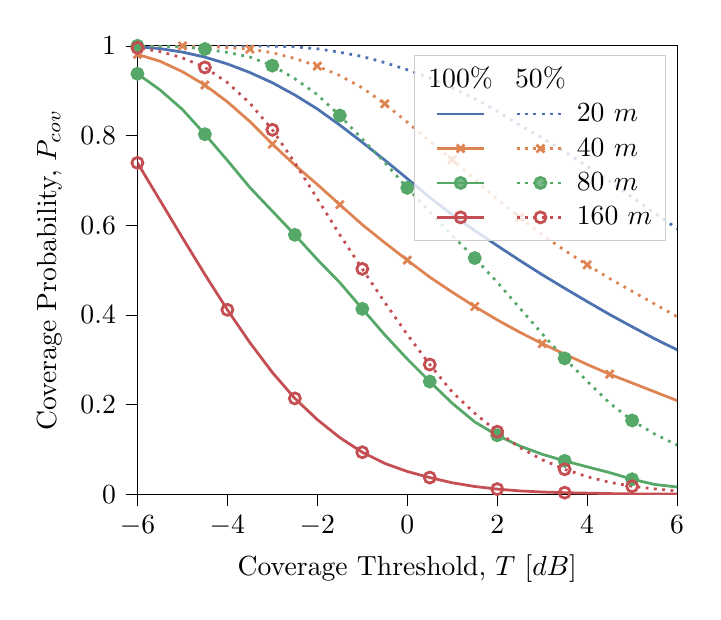
\begin{tikzpicture}

\definecolor{color0}{rgb}{0.298039215686275,0.447058823529412,0.690196078431373}
\definecolor{color1}{rgb}{0.866666666666667,0.517647058823529,0.32156862745098}
\definecolor{color2}{rgb}{0.333333333333333,0.658823529411765,0.407843137254902}
\definecolor{color3}{rgb}{0.768627450980392,0.305882352941176,0.32156862745098}

\begin{axis}[
legend cell align={left},
legend style={fill opacity=0.8, draw opacity=1, text opacity=1, draw=white!80!black},
legend columns=2,
legend style={
    font=\mystrut,
    legend cell align=left,
},
tick align=outside,
tick pos=left,
x grid style={white!69.0196078431373!black},
xlabel={Coverage Threshold, $T$ [$dB$]},
xmin=-6, xmax=6,
xtick style={color=black},
y grid style={white!69.0196078431373!black},
ylabel={Coverage Probability, $P_{cov}$},
ymin=0, ymax=1,
ytick style={color=black}
]
\addlegendimage{legend image with text=$100\%$}
\addlegendentry{}
% column 2 heading
\addlegendimage{legend image with text=$50\%$}
\addlegendentry{}
\addplot [line width=1.0pt, color0]
table {%
-7 0.999977231025696
-6.5 0.999641180038452
-6 0.998011827468872
-5.5 0.993778944015503
-5 0.986085176467896
-4.5 0.974705457687378
-4 0.959611415863037
-3.5 0.940409660339355
-3 0.917675971984863
-2.5 0.890339136123657
-2 0.859145402908325
-1.5 0.823200345039368
-1 0.784802794456482
-0.5 0.744963884353638
0 0.703732013702393
0.5 0.661916375160217
1 0.623131394386292
1.5 0.587850093841553
2 0.554275035858154
2.5 0.521309494972229
3 0.489463448524475
3.5 0.459146976470947
4 0.429608345031738
4.5 0.400633573532104
5 0.373367786407471
5.5 0.346626281738281
6 0.321901440620422
6.5 0.300284266471863
};
\addlegendentry{}
\addplot [line width=1.0pt, color0, dotted]
table {%
-7 1
-3.5 0.999866127967834
-3 0.999324917793274
-2.5 0.997615814208984
-2 0.993337392807007
-1.5 0.985663652420044
-1 0.976215124130249
-0.5 0.962559461593628
0 0.946608066558838
0.5 0.92812705039978
1 0.906381726264954
1.5 0.882081270217896
2 0.85400390625
2.5 0.823311448097229
3 0.794575929641724
3.5 0.763923406600952
4 0.731695652008057
4.5 0.697926878929138
5 0.662343621253967
6 0.592154145240784
6.5 0.557505130767822
};
\addlegendentry{$20~m$}
\addplot [line width=1.0pt, color1, mark=x, mark repeat={3}, mark options={solid}]
table {%
-7 0.995241403579712
-6.5 0.990424513816833
-6 0.980918645858765
-5.5 0.965644478797913
-5 0.942358016967773
-4.5 0.912482976913452
-4 0.874948501586914
-3.5 0.831153869628906
-3 0.780678749084473
-2.5 0.733933329582214
-2 0.690728187561035
-1.5 0.645623564720154
-1 0.601058483123779
-0.5 0.560723543167114
0 0.521915435791016
0.5 0.483930587768555
1 0.450548410415649
1.5 0.418470740318298
2 0.38869297504425
2.5 0.361095666885376
3 0.335737228393555
3.5 0.312261581420898
4 0.2893226146698
4.5 0.267479538917542
6 0.208658218383789
6.5 0.190708756446838
};
\addlegendentry{}
\addplot [line width=1.0pt, color1, dotted, mark=x, mark repeat={3}, mark options={solid}]
table {%
-7 1
-5 0.999666213989258
-4.5 0.998450875282288
-4 0.996201038360596
-3.5 0.992630004882812
-3 0.984634160995483
-2.5 0.971801996231079
-2 0.954736828804016
-1.5 0.933683633804321
-1 0.906353235244751
-0.5 0.870607137680054
0 0.829646468162537
0.5 0.787314653396606
1 0.746014595031738
1.5 0.702292203903198
2 0.658163785934448
2.5 0.61738383769989
3 0.578600764274597
3.5 0.543644547462463
4 0.511425018310547
4.5 0.480882406234741
6 0.395854473114014
6.5 0.369149923324585
};
\addlegendentry{$40~m$}
\addplot [line width=1.0pt, color2, mark=*, mark repeat={3}, mark options={solid}]
table {%
-7 0.980716705322266
-6.5 0.964327812194824
-6 0.937661170959473
-5.5 0.901883363723755
-5 0.858041644096375
-4.5 0.802763938903809
-4 0.744447231292725
-3.5 0.683861136436462
-2.5 0.578400015830994
-2 0.523316621780396
-1.5 0.471825003623962
-1 0.413255572319031
-0.5 0.355283260345459
0 0.301361083984375
0.5 0.25106942653656
1 0.202663898468018
1.5 0.161088943481445
2 0.131269454956055
2.5 0.107397198677063
3 0.0889694690704346
3.5 0.0742361545562744
4 0.0608916282653809
4.5 0.0480166673660278
5 0.033227801322937
5.5 0.021588921546936
6 0.0159167051315308
6.5 0.0122444629669189
};
\addlegendentry{}
\addplot [line width=1.0pt, color2, dotted, mark=*, mark repeat={3}, mark options={solid}]
table {%
-7 1
-6 0.999997138977051
-5.5 0.999533414840698
-5 0.997600078582764
-4.5 0.99286675453186
-4 0.9852694272995
-3.5 0.97504448890686
-3 0.955780506134033
-2.5 0.926708340644836
-2 0.890936136245728
-1.5 0.844488859176636
-1 0.791713953018188
-0.5 0.739855527877808
0 0.683194398880005
0.5 0.629683256149292
1 0.576952695846558
1.5 0.526600003242493
2 0.47278892993927
3 0.357519388198853
3.5 0.302783370018005
4 0.251888871192932
4.5 0.203147172927856
5 0.164294481277466
5.5 0.134108304977417
6 0.109505534172058
6.5 0.0909055471420288
};
\addlegendentry{$80~m$}
\addplot [line width=1.0pt, color3, mark=o, mark repeat={3}, mark options={solid}]
table {%
-7 0.87862491607666
-6.5 0.816091656684875
-6 0.73895001411438
-5 0.572083353996277
-4.5 0.489966630935669
-4 0.411166667938232
-3.5 0.337991714477539
-3 0.271308302879333
-2.5 0.213508367538452
-2 0.166169404983521
-1.5 0.126036167144775
-1 0.093447208404541
-0.5 0.0684916973114014
0 0.0505222082138062
0.5 0.0370138883590698
1 0.0253027677536011
1.5 0.0170778036117554
2 0.0112360715866089
2.5 0.00719165802001953
3 0.00472497940063477
3.5 0.00319719314575195
4.5 0.00118339061737061
5 0.000552773475646973
6.5 2.50339508056641e-05
};
\addlegendentry{}
\addplot [line width=1.0pt, color3, dotted, mark=o, mark repeat={3}, mark options={solid}]
table {%
-7 0.999927759170532
-6.5 0.999477863311768
-6 0.995466709136963
-5.5 0.987174987792969
-5 0.973161101341248
-4.5 0.951763868331909
-4 0.917977809906006
-3.5 0.8719722032547
-3 0.812672138214111
-2.5 0.739083290100098
-1.5 0.578566670417786
-1 0.502369403839111
-0.5 0.427655577659607
0 0.355913877487183
0.5 0.289049983024597
1 0.227694511413574
1.5 0.180425047874451
2 0.139313936233521
2.5 0.104269504547119
3 0.0766305923461914
3.5 0.0554111003875732
4 0.0388027429580688
4.5 0.0263082981109619
5 0.0175639390945435
5.5 0.0116583108901978
6 0.00716948509216309
6.5 0.00450277328491211
};
\addlegendentry{$160~m$}
\end{axis}

\end{tikzpicture}

	}
	\caption{Impact of the outage threshold, $T$, on the coverage probability, $P_{cov}$ at different altitudes under a $50\%$ or a $100\%$ network load.}
	\label{fig:leuven_cov_vs_threshold}
\end{figure}

%\subsubsection{Multi-Operator}
\par In an effort to solve this coverage problem, we consider a connection with multiple networks at the same time. The SINR values in this network are calculated using \eqref{eq:sinr_max}.
The coverage probability as a function of the drone altitude can be seen in Fig. \ref{fig:leuven_multi_cov}. When using one network operator, the probability stays one up until around $20~m$ height as the network is designed this way. However, we can see the coverage drops as soon as the UAV flies above rooftop height. In a multi-operator network we can see that the 100\% coverage reaches a much higher altitude. At an altitude of $100~m$ the coverage probability in a multi-operator network is still 0.99. This altitude is much more likely to be used by a drone network. Above this altitude the coverage drops again, albeit less than with one operator. The increase in coverage probability from using two compared to using three operators is less but can be considered for ultra-reliable systems. %The slight increase in coverage probability around $100~m$ can be explained by the sidelobe suppression of the antennas.


\begin{figure}[]
    \centering % <-- added
    % \begin{subfigure}{\linewidth}
    %     \includegraphics[width=\linewidth]{img/leuven/multi_sinr_vs_h.pdf}
    %     \caption{Average SINR}
    %     \label{fig:leuven_multi_sinr}
    % \end{subfigure}\hfil % <-- added
    
	\resizebox{0.9\linewidth}{!}{
    \begin{subfigure}{\linewidth}
        % This file was created by tikzplotlib v0.9.4.
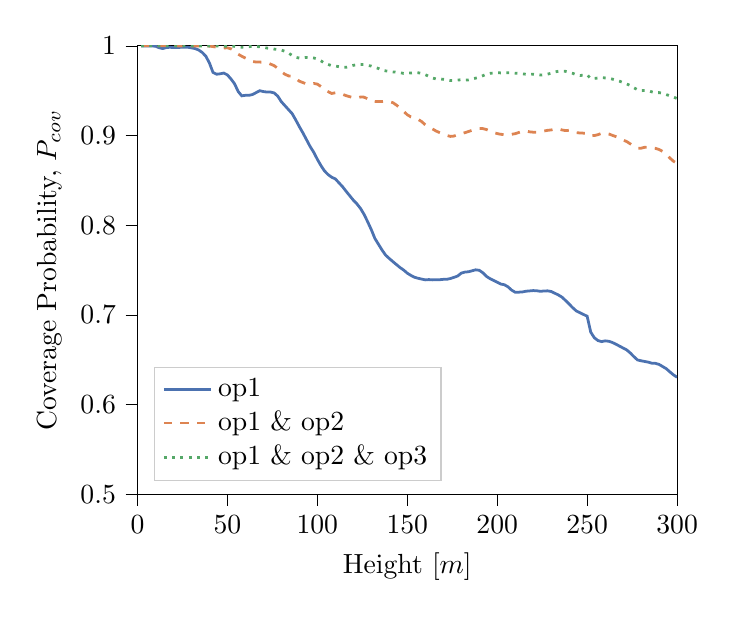
\begin{tikzpicture}

\definecolor{color0}{rgb}{0.298039215686275,0.447058823529412,0.690196078431373}
\definecolor{color1}{rgb}{0.866666666666667,0.517647058823529,0.32156862745098}
\definecolor{color2}{rgb}{0.333333333333333,0.658823529411765,0.407843137254902}

\begin{axis}[
legend cell align={left},
legend style={fill opacity=0.8, draw opacity=1, text opacity=1, at={(0.03,0.03)}, anchor=south west, draw=white!80!black},
tick align=outside,
tick pos=left,
x grid style={white!69.0196078431373!black},
xlabel={Height [$m$]},
xmin=0, xmax=300,
xtick style={color=black},
y grid style={white!69.0196078431373!black},
ylabel={Coverage Probability, $P_{cov}$},
ymin=0.5, ymax=1,
ytick style={color=black}
]
\addplot [line width=1.0pt, color0]
table {%
2 0.999848365783691
6 0.999863147735596
10 0.999586582183838
12 0.997876405715942
14 0.996934294700623
16 0.997975945472717
18 0.998380422592163
20 0.998011827468872
22 0.99799108505249
24 0.998309373855591
26 0.998451471328735
28 0.998361229896545
30 0.997753143310547
32 0.996879100799561
34 0.995389938354492
36 0.992586612701416
38 0.988445997238159
40 0.980918645858765
42 0.970294713973999
44 0.968319892883301
46 0.968779444694519
48 0.969600439071655
50 0.96755838394165
52 0.962995409965515
54 0.957619667053223
56 0.949039816856384
58 0.944198250770569
60 0.944767475128174
62 0.944751024246216
64 0.945707440376282
68 0.949952244758606
70 0.948944091796875
72 0.948430299758911
74 0.948441386222839
76 0.947446942329407
78 0.943852782249451
80 0.937661170959473
86 0.924355506896973
88 0.917308330535889
90 0.909850001335144
92 0.902824997901917
96 0.887647151947021
98 0.881272196769714
100 0.873461127281189
102 0.866491675376892
104 0.860411167144775
106 0.856349945068359
108 0.853419423103333
110 0.851569414138794
114 0.8429194688797
116 0.837774991989136
120 0.827866673469543
122 0.823722243309021
124 0.818630576133728
126 0.81196117401123
128 0.803672194480896
130 0.794977784156799
132 0.785152792930603
136 0.772136092185974
138 0.766466617584229
140 0.762786149978638
142 0.759319424629211
146 0.752658367156982
148 0.749902725219727
150 0.746427774429321
152 0.743958353996277
154 0.741883277893066
156 0.740716695785522
160 0.73895001411438
162 0.739269495010376
164 0.73895001411438
168 0.73913049697876
170 0.739536046981812
172 0.739613890647888
174 0.740447282791138
176 0.741761088371277
178 0.743222236633301
180 0.74643611907959
182 0.747616648674011
184 0.747986078262329
188 0.750149965286255
190 0.749655485153198
192 0.74691104888916
194 0.74293053150177
196 0.740299940109253
202 0.734263896942139
204 0.733522176742554
206 0.731177806854248
208 0.727561116218567
210 0.725158333778381
212 0.725230574607849
214 0.725499987602234
216 0.726288914680481
220 0.727002859115601
222 0.726808309555054
224 0.726188898086548
226 0.726555585861206
228 0.72670841217041
230 0.72599720954895
234 0.722130537033081
236 0.719680547714233
238 0.715938806533813
242 0.707886099815369
244 0.704238891601562
250 0.698400020599365
252 0.68060827255249
254 0.674375057220459
256 0.671277761459351
258 0.670102834701538
260 0.670919418334961
262 0.670483350753784
264 0.669125080108643
266 0.667191743850708
272 0.660813808441162
274 0.657369375228882
276 0.653322219848633
278 0.649625062942505
280 0.648708343505859
284 0.647186040878296
286 0.645966649055481
288 0.645822286605835
290 0.644638895988464
294 0.639869451522827
296 0.636311054229736
298 0.632977724075317
300 0.630294442176819
};
\addlegendentry{op1}
\addplot [line width=1.0pt, color1, dashed]
table {%
2 1
38 0.9998859167099
40 0.999644041061401
42 0.999160170555115
44 0.998479127883911
46 0.996949911117554
48 0.997620344161987
50 0.997759580612183
52 0.99660062789917
54 0.994436740875244
56 0.990637063980103
58 0.988345623016357
62 0.984271764755249
64 0.982505321502686
66 0.981910943984985
68 0.981872081756592
72 0.981274843215942
76 0.977877616882324
78 0.97480833530426
80 0.971061110496521
82 0.968269467353821
84 0.966441631317139
86 0.965886116027832
88 0.963663816452026
90 0.960555553436279
92 0.958969473838806
94 0.957572221755981
96 0.957158327102661
98 0.958047151565552
100 0.957294464111328
102 0.954622268676758
104 0.950950026512146
108 0.946836113929749
110 0.947644472122192
112 0.947197198867798
114 0.946005582809448
116 0.944383382797241
118 0.943258285522461
120 0.941961050033569
122 0.941711187362671
124 0.942872285842896
126 0.942744493484497
128 0.940805554389954
130 0.938127756118774
132 0.937769412994385
134 0.937936067581177
136 0.93785548210144
138 0.938063859939575
140 0.937644481658936
142 0.936597228050232
144 0.933880567550659
146 0.9305499792099
150 0.923141717910767
152 0.920697212219238
154 0.919813871383667
156 0.917949914932251
158 0.915502786636353
160 0.911922216415405
162 0.909344434738159
164 0.907291650772095
166 0.904966592788696
170 0.901400089263916
172 0.900008320808411
174 0.898961067199707
176 0.899344444274902
178 0.90084445476532
180 0.901822209358215
188 0.906975030899048
190 0.90785551071167
192 0.907666683197021
194 0.906655550003052
198 0.9032222032547
200 0.902119398117065
202 0.901274919509888
204 0.901058316230774
208 0.901294469833374
210 0.90202784538269
214 0.904716730117798
216 0.904961109161377
218 0.904047250747681
220 0.903666734695435
222 0.903508305549622
224 0.903741598129272
226 0.904947280883789
228 0.905719518661499
230 0.906158328056335
232 0.907161116600037
234 0.907327771186829
236 0.906166672706604
238 0.905430555343628
240 0.905769467353821
242 0.904830574989319
244 0.903172254562378
246 0.902775049209595
248 0.902588844299316
250 0.902602791786194
252 0.899769425392151
254 0.89989161491394
256 0.900877714157104
258 0.902394533157349
260 0.902619361877441
262 0.901744365692139
264 0.900150060653687
266 0.898725032806396
268 0.897050023078918
270 0.894941687583923
272 0.893199920654297
276 0.888044357299805
278 0.885841608047485
280 0.885819435119629
282 0.886797189712524
284 0.887088894844055
286 0.886224985122681
288 0.885591745376587
290 0.884366750717163
292 0.882180571556091
294 0.878775000572205
296 0.874808311462402
298 0.871230602264404
300 0.868858337402344
};
\addlegendentry{op1 \& op2}
\addplot [line width=1.0pt, color2, dotted]
table {%
2 1
44 0.999908208847046
46 0.999510645866394
52 0.999727606773376
54 0.999441385269165
56 0.998546957969666
58 0.998422026634216
64 0.999366641044617
66 0.999316692352295
70 0.998363852500916
72 0.997463941574097
74 0.997174978256226
76 0.996350049972534
78 0.995947241783142
80 0.995208263397217
82 0.99382221698761
84 0.99192214012146
86 0.989163875579834
88 0.987197160720825
90 0.986313819885254
92 0.986816644668579
94 0.986897230148315
96 0.986791610717773
98 0.98645555973053
100 0.985330581665039
102 0.983252763748169
104 0.980561137199402
106 0.979255557060242
108 0.97771942615509
110 0.977452754974365
112 0.976730585098267
114 0.976150035858154
116 0.976000070571899
120 0.978241682052612
122 0.978916645050049
124 0.979305505752563
126 0.979052782058716
128 0.978124976158142
130 0.977402806282043
132 0.975908279418945
134 0.974711179733276
136 0.972641706466675
142 0.97088885307312
144 0.970669507980347
146 0.970013856887817
148 0.969216585159302
154 0.969966650009155
156 0.969908356666565
158 0.969366669654846
160 0.967777729034424
164 0.964149951934814
166 0.962991714477539
168 0.963022232055664
170 0.962683320045471
174 0.961266756057739
176 0.961277723312378
178 0.961791753768921
180 0.962144374847412
182 0.961841583251953
184 0.96197497844696
190 0.964908361434937
194 0.968341588973999
196 0.969247221946716
198 0.969708323478699
200 0.969991683959961
202 0.969783306121826
206 0.969963908195496
208 0.969758272171021
210 0.969408273696899
212 0.969261169433594
216 0.968286037445068
218 0.96797776222229
220 0.96839165687561
222 0.968199968338013
224 0.967472195625305
226 0.9676833152771
228 0.968430519104004
230 0.96940279006958
232 0.970844507217407
234 0.971605539321899
236 0.971763849258423
238 0.971499919891357
242 0.969308376312256
244 0.967716693878174
246 0.966899991035461
248 0.967216730117798
250 0.967747211456299
252 0.963325023651123
254 0.96358335018158
258 0.964577794075012
262 0.963738918304443
264 0.962877750396729
268 0.960522174835205
272 0.95746111869812
274 0.955688953399658
276 0.953202724456787
278 0.950955629348755
280 0.949944496154785
282 0.950205564498901
284 0.949963808059692
286 0.948572158813477
288 0.947780609130859
290 0.947786092758179
292 0.947041749954224
300 0.941291689872742
};
\addlegendentry{op1 \& op2 \& op3}
\end{axis}

\end{tikzpicture}

        \caption{Coverage probability $P_{cov}$}
        \label{fig:leuven_multi_cov}
    \end{subfigure}} % <-- added
    \resizebox{0.9\linewidth}{!}{
    \begin{subfigure} {\linewidth}
        % This file was created by tikzplotlib v0.9.4.
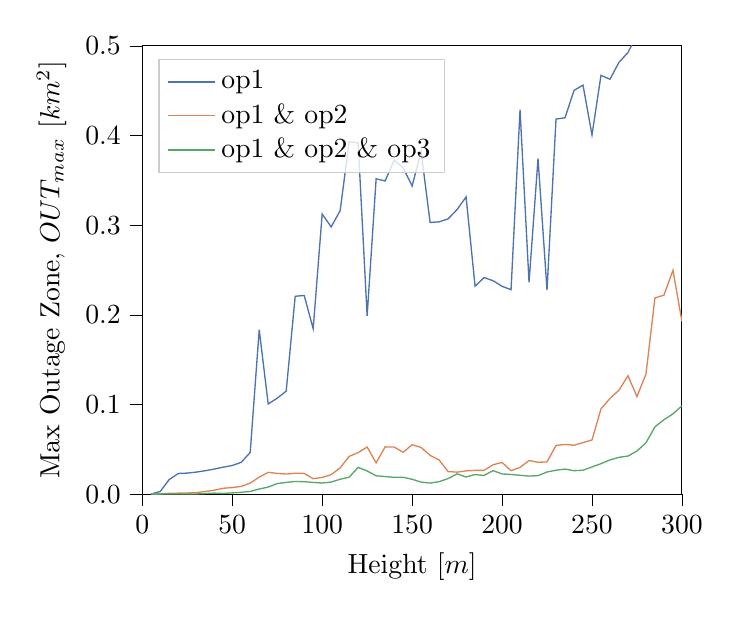
\begin{tikzpicture}

\definecolor{color0}{rgb}{0.298039215686275,0.447058823529412,0.690196078431373}
\definecolor{color1}{rgb}{0.866666666666667,0.517647058823529,0.32156862745098}
\definecolor{color2}{rgb}{0.333333333333333,0.658823529411765,0.407843137254902}

\begin{axis}[
legend cell align={left},
legend style={fill opacity=0.8, draw opacity=1, text opacity=1, at={(0.03,0.97)}, anchor=north west, draw=white!80!black},
tick align=outside,
tick pos=left,
x grid style={white!69.0196078431373!black},
xlabel={Height [$m$]},
xmin=0, xmax=300,
xtick style={color=black},
y grid style={white!69.0196078431373!black},
ylabel={Max Outage Zone, $OUT_{max}$ [$km^2$]},
ymin=0.0, ymax=0.5,
yticklabel style={%
                 /pgf/number format/.cd,
                     fixed,
                     fixed zerofill,
                     precision=1,},
ytick style={color=black}
]
\addplot [line width=0.48pt, color0]
table {%
5 6.34193420410156e-05
10 0.00301218032836914
15 0.0163115262985229
20 0.0230492353439331
25 0.0234367847442627
30 0.0245600938796997
35 0.0261001586914062
40 0.0279483795166016
45 0.030073881149292
50 0.0318921804428101
55 0.0354760885238647
60 0.0465353727340698
65 0.183377742767334
70 0.100533366203308
75 0.106977820396423
80 0.114888906478882
85 0.220666646957397
90 0.221555590629578
95 0.184488892555237
100 0.312444448471069
105 0.297999978065491
110 0.316177845001221
115 0.393022179603577
120 0.391866683959961
125 0.198711156845093
130 0.351688861846924
135 0.349200010299683
140 0.37244439125061
145 0.364088892936707
150 0.343644380569458
155 0.382177829742432
160 0.302977800369263
165 0.303688883781433
170 0.30697774887085
175 0.317422151565552
180 0.331422209739685
185 0.231866717338562
190 0.241466641426086
195 0.238044500350952
200 0.231777787208557
205 0.22795557975769
210 0.428711175918579
215 0.236088871955872
220 0.374311089515686
225 0.227466702461243
230 0.418355584144592
235 0.419688940048218
240 0.450266599655151
245 0.456133365631104
250 0.400622248649597
255 0.467022180557251
260 0.462711095809937
265 0.481600046157837
270 0.492488861083984
275 0.512444496154785
280 0.516799926757812
290 0.530133247375488
295 0.534311056137085
300 0.543288946151733
};
\addlegendentry{op1}
\addplot [line width=0.48pt, color1]
table {%
5 4.44650650024414e-05
10 0.000311136245727539
15 0.000888943672180176
25 0.00128889083862305
30 0.00164449214935303
40 0.00431108474731445
45 0.00653338432312012
50 0.00733327865600586
55 0.00862216949462891
60 0.0122666358947754
65 0.0189332962036133
70 0.0242667198181152
75 0.02311110496521
80 0.0223555564880371
85 0.0233333110809326
90 0.0230666399002075
95 0.0172444581985474
100 0.0186222791671753
105 0.0216889381408691
110 0.0292888879776001
115 0.0421333312988281
120 0.0463111400604248
125 0.0525333881378174
130 0.03493332862854
135 0.0526666641235352
140 0.0525333881378174
145 0.0466222763061523
150 0.0551111698150635
155 0.0520443916320801
160 0.0432889461517334
165 0.0380444526672363
170 0.0251555442810059
175 0.0244889259338379
180 0.0259110927581787
185 0.0264889001846313
190 0.0264889001846313
195 0.0327556133270264
200 0.0353332757949829
205 0.0261332988739014
210 0.0298222303390503
215 0.0375111103057861
220 0.0354666709899902
225 0.035955548286438
230 0.0543111562728882
235 0.0554221868515015
240 0.0545333623886108
250 0.0604000091552734
255 0.0951111316680908
260 0.106711149215698
265 0.11591112613678
270 0.132044434547424
275 0.108800053596497
280 0.133866667747498
285 0.218799948692322
290 0.221911072731018
295 0.24964439868927
300 0.19266664981842
};
\addlegendentry{op1 \& op2}
\addplot [line width=0.48pt, color2]
table {%
5 0
30 0.000177741050720215
40 0.00111114978790283
45 0.000755548477172852
55 0.00199997425079346
60 0.00297772884368896
65 0.00568890571594238
70 0.00786662101745605
75 0.0117777585983276
80 0.0130666494369507
85 0.0141333341598511
90 0.013866662979126
95 0.0130221843719482
100 0.0124000310897827
105 0.0134667158126831
110 0.0165777206420898
115 0.0189332962036133
120 0.0297777652740479
125 0.0258221626281738
130 0.020444393157959
140 0.0187110900878906
145 0.0188000202178955
150 0.016533374786377
155 0.0134222507476807
160 0.0123111009597778
165 0.013866662979126
170 0.0173333883285522
175 0.0226222276687622
180 0.0190666913986206
185 0.0218666791915894
190 0.020799994468689
195 0.0262222290039062
200 0.0224888324737549
205 0.0219111442565918
215 0.0200889110565186
220 0.0206222534179688
225 0.0246666669845581
230 0.0265778303146362
235 0.0279110670089722
240 0.0260888338088989
245 0.0266666412353516
255 0.0339555740356445
260 0.0381333827972412
265 0.0410221815109253
270 0.0424444675445557
275 0.0480889081954956
280 0.0571999549865723
285 0.0750666856765747
290 0.0829777717590332
295 0.0895111560821533
300 0.0983999967575073
};
\addlegendentry{op1 \& op2 \& op3}
\end{axis}

\end{tikzpicture}

        \caption{Maximum outage zone $OUT_{max}$}
        \label{fig:leuven_multi_outmax}
    \end{subfigure} % <-- added
    }
    \caption{Impact of multi-operator diversity on the network performance. Using multiple cellular networks enables UAV connectivity at higher altitudes.}
\end{figure}

\par Fig. \ref{fig:leuven_multi_outmax} shows the $OUT_{max}$ as function of the altitude. Using a single operator results in relatively large outage zones, especially at altitudes above $100~m$. In a multi-operator scenario the size of the outage zones stays relatively small even at very large altitudes. A single operator network experiences much larger continuous outage zones than a two or three operator network. This can be explained by the fact that many of the antenna sites are different for the selection operators and even if they utilize the same antenna site they often deploy their sectors with different infrastructure, resulting in different azimuths, tilts, etc. 



\subsection{Handovers}
\par The assignment map indicates which sector has the highest received power at each point. In Fig. \ref{fig:leuven_assmap} the assignment map of two operators at different altitudes is shown. Each color represents a sector, meaning that the color of a pixel determines which sector a user is assigned to at this location. One can observe that at $120~m$ height the assignment pattern is much more fragmented than the one at $20~m$ height. Due to the antenna sidelobes and nulls, UAVs at high altitudes will connect to sectors that are not necessarily the closest or they will alternate rapidly between multiple sectors. This will lead to higher handover frequency. These handovers result in throughput drops, where at these altitudes throughput is already a scarce resource. To build a reliable UAV communications network, reducing the number of handovers and Radio-Link-Failures is in the best of interest. 
\begin{figure}
	\centering
    \begin{subfigure}[b]{0.49\linewidth}
        \centering
        \includegraphics[width=\textwidth]{img/leuven/ass-pxs-20m.pdf}
        \caption{Operator 1, $20~m$}
    \end{subfigure}
    \hfill
    \begin{subfigure}[b]{0.49\linewidth}
        \centering
        \includegraphics[width=\textwidth]{img/leuven/ass-pxs-120m.pdf}
        \caption{Operator 1, $120~m$}
    \end{subfigure}
    \vfill
	\begin{subfigure}[b]{0.49\linewidth}
    \centering
    \includegraphics[width=\textwidth]{img/leuven/ass-tnt-20m.pdf}
        \caption{Operator 2, $20~m$}
    \end{subfigure}
    \hfill
	\begin{subfigure}[b]{0.49\linewidth}
    \centering
    \includegraphics[width=\textwidth]{img/leuven/ass-tnt-120m.pdf}
        \caption{Operator 2, $120~m$}
    \end{subfigure}
	    \caption{Sector assignment map for two network operators at $20~m$ and $120~m$ height. Each color represents a different sector. The color of a pixel indicates which sector a user at this location is assigned to.}
     \label{fig:leuven_assmap}
\end{figure}
%\subsubsection{Multi-operator}
Fig. \ref{fig:leuven_assmap} also shows the difference in assignment patterns between two different operators. We can utilize this diversity to create a multi-operator network where when a handover needs to happen or when a RLF occurs, the user can always fall back on the other operator's network.

%\par As in this scenario when a handover from one sector to another is required or a RLF is experienced in a specific operator's network, there is a low probability that this will not be the case in another operator's network at exactly the same time and or location. Therefore, being connected to multiple operator's networks at the same time will reduce handover and RLF rates.

\par The results can be neatly observed in the Fig. \ref{fig:handovers_results}. Fig. \ref{fig:handovers_time} shows the  handover frequency experienced by a drone flying at certain altitudes. When looking at a single operator system, we can see that a drone flying at an altitude of $160~m$ experiences a median of five handovers, this is a handover every 12 seconds. It is clear that this will cause significant problems for the command and control link. In contrast, the multi operator systems experience approximately zero handovers at the same altitude, due to the network diversity.
\par The same positive effect can be seen when monitoring the RLF duration. Fig. \ref{fig:rlf_dur} shows the duration a drone will not be connected to the network when it encounters a RLF. At an altitude of $160~m$ a drone using a single network will have a median disconnection time of $4~s$ when encountering a no-coverage zone. This is clearly not a desired situation. However, a drone connecting to multiple networks simultaneously can bring down this duration to a median of $1~s$. This shows the clear benefits for drones of connecting to multiple cellular networks at the same time.
%\par It is clear that a UAV can greatly reduce the number of problematic handovers by connecting to multiple cellular networks simultaneously, while also reducing the time spent disconnected from the network due to RLF.


\label{sec:handovers}
\begin{figure}[]
    \centering % <-- added
    
    \resizebox{0.825\linewidth}{!}{
    \begin{subfigure}{0.9\linewidth}
        % \includegraphics[width=\linewidth]{img/handovers/box_outage.pdf}
        % This file was created by tikzplotlib v0.9.4.
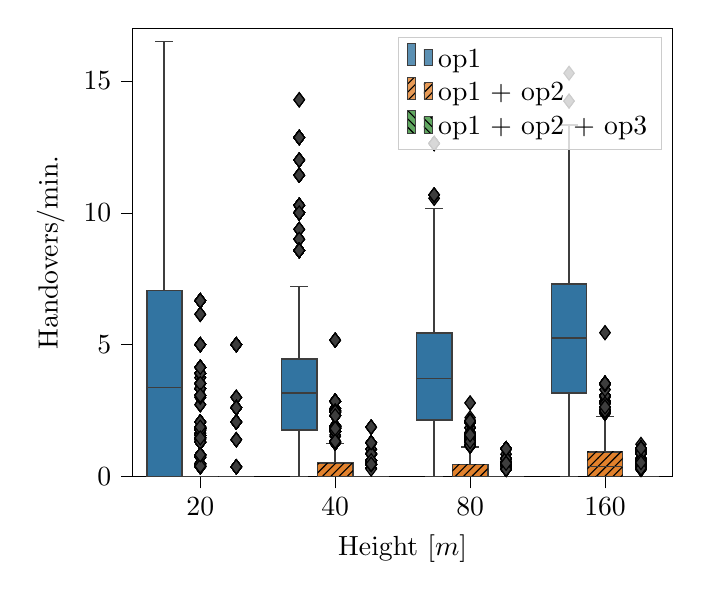
\begin{tikzpicture}

\definecolor{color0}{rgb}{0.194607843137255,0.453431372549019,0.632843137254902}
\definecolor{color1}{rgb}{0.881862745098039,0.505392156862745,0.173039215686275}
\definecolor{color2}{rgb}{0.229411764705882,0.570588235294118,0.229411764705882}

\begin{axis}[
legend cell align={left},
legend style={fill opacity=0.8, draw opacity=1, text opacity=1, draw=white!80!black},
tick align=outside,
tick pos=left,
x grid style={white!69.0196078431373!black},
xlabel={Height [$m$]},
xmin=-0.5, xmax=3.5,
xtick style={color=black},
xtick={0,1,2,3},
xticklabels={20,40,80,160},
y grid style={white!69.0196078431373!black},
ylabel={Handovers/min.},
ymin=0, ymax=17,
ytick style={color=black}
]
\path [draw=white!23.921568627451!black, fill=color0, semithick]
(axis cs:-0.397333333333333,0)
--(axis cs:-0.136,0)
--(axis cs:-0.136,7.05882358551025)
--(axis cs:-0.397333333333333,7.05882358551025)
--(axis cs:-0.397333333333333,0)
--cycle;
\path [draw=white!23.921568627451!black, fill=color1, semithick][postaction={pattern=north east lines}]
(axis cs:-0.130666666666667,0)
--(axis cs:0.130666666666667,0)
--(axis cs:0.130666666666667,0)
--(axis cs:-0.130666666666667,0)
--(axis cs:-0.130666666666667,0)
--cycle;
\path [draw=white!23.921568627451!black, fill=color2, semithick][postaction={pattern=north west lines}]
(axis cs:0.136,0)
--(axis cs:0.397333333333333,0)
--(axis cs:0.397333333333333,0)
--(axis cs:0.136,0)
--(axis cs:0.136,0)
--cycle;
\path [draw=white!23.921568627451!black, fill=color0, semithick]
(axis cs:0.602666666666667,1.76470589637756)
--(axis cs:0.864,1.76470589637756)
--(axis cs:0.864,4.46808528900146)
--(axis cs:0.602666666666667,4.46808528900146)
--(axis cs:0.602666666666667,1.76470589637756)
--cycle;
\path [draw=white!23.921568627451!black, fill=color1, semithick][postaction={pattern=north east lines}]
(axis cs:0.869333333333333,0)
--(axis cs:1.13066666666667,0)
--(axis cs:1.13066666666667,0.508474588394165)
--(axis cs:0.869333333333333,0.508474588394165)
--(axis cs:0.869333333333333,0)
--cycle;
\path [draw=white!23.921568627451!black, fill=color2, semithick][postaction={pattern=north west lines}]
(axis cs:1.136,0)
--(axis cs:1.39733333333333,0)
--(axis cs:1.39733333333333,0)
--(axis cs:1.136,0)
--(axis cs:1.136,0)
--cycle;
\path [draw=white!23.921568627451!black, fill=color0, semithick]
(axis cs:1.60266666666667,2.14285707473755)
--(axis cs:1.864,2.14285707473755)
--(axis cs:1.864,5.45454549789429)
--(axis cs:1.60266666666667,5.45454549789429)
--(axis cs:1.60266666666667,2.14285707473755)
--cycle;
\path [draw=white!23.921568627451!black, fill=color1, semithick][postaction={pattern=north east lines}]
(axis cs:1.86933333333333,0)
--(axis cs:2.13066666666667,0)
--(axis cs:2.13066666666667,0.45284940302372)
--(axis cs:1.86933333333333,0.45284940302372)
--(axis cs:1.86933333333333,0)
--cycle;
\path [draw=white!23.921568627451!black, fill=color2, semithick][postaction={pattern=north west lines}]
(axis cs:2.136,0)
--(axis cs:2.39733333333333,0)
--(axis cs:2.39733333333333,0)
--(axis cs:2.136,0)
--(axis cs:2.136,0)
--cycle;
\path [draw=white!23.921568627451!black, fill=color0, semithick]
(axis cs:2.60266666666667,3.16629350185394)
--(axis cs:2.864,3.16629350185394)
--(axis cs:2.864,7.29617750644684)
--(axis cs:2.60266666666667,7.29617750644684)
--(axis cs:2.60266666666667,3.16629350185394)
--cycle;
\path [draw=white!23.921568627451!black, fill=color1, semithick][postaction={pattern=north east lines}]
(axis cs:2.86933333333333,0)
--(axis cs:3.13066666666667,0)
--(axis cs:3.13066666666667,0.9375)
--(axis cs:2.86933333333333,0.9375)
--(axis cs:2.86933333333333,0)
--cycle;
\path [draw=white!23.921568627451!black, fill=color2, semithick][postaction={pattern=north west lines}]
(axis cs:3.136,0)
--(axis cs:3.39733333333333,0)
--(axis cs:3.39733333333333,0)
--(axis cs:3.136,0)
--(axis cs:3.136,0)
--cycle;
\draw[draw=white!23.921568627451!black,fill=color0,line width=0.3pt] (axis cs:0,0) rectangle (axis cs:0,0);
\addlegendimage{ybar,ybar legend,draw=white!23.921568627451!black,fill=color0,line width=0.3pt};
\addlegendentry{op1}

\draw[draw=white!23.921568627451!black,fill=color1,line width=0.3pt] (axis cs:0,0) rectangle (axis cs:0,0);
\addlegendimage{ybar,ybar legend,draw=white!23.921568627451!black,fill=color1,line width=0.3pt,postaction={pattern=north east lines}};
\addlegendentry{op1 + op2}

\draw[draw=white!23.921568627451!black,fill=color2,line width=0.3pt] (axis cs:0,0) rectangle (axis cs:0,0);
\addlegendimage{ybar,ybar legend,draw=white!23.921568627451!black,fill=color2,line width=0.3pt,postaction={pattern=north west lines}};
\addlegendentry{op1 + op2 + op3}

\addplot [semithick, white!23.921568627451!black, forget plot]
table {%
-0.266666650772095 0
-0.266666650772095 0
};
\addplot [semithick, white!23.921568627451!black, forget plot]
table {%
-0.266666650772095 7.05882358551025
-0.266666650772095 16.5
};
\addplot [semithick, white!23.921568627451!black, forget plot]
table {%
-0.332000017166138 0
-0.201333284378052 0
};
\addplot [semithick, white!23.921568627451!black, forget plot]
table {%
-0.332000017166138 16.5
-0.201333284378052 16.5
};
\addplot [black, mark=diamond*, mark size=2.5, mark options={solid,fill=white!23.921568627451!black}, only marks, forget plot]
table {%
-0.266666650772095 40
-0.266666650772095 20
-0.266666650772095 30
-0.266666650772095 20
-0.266666650772095 40
-0.266666650772095 20
-0.266666650772095 30
-0.266666650772095 40
-0.266666650772095 20
-0.266666650772095 30
-0.266666650772095 20
-0.266666650772095 40
-0.266666650772095 30
-0.266666650772095 20
-0.266666650772095 40
-0.266666650772095 20
-0.266666650772095 30
-0.266666650772095 20
-0.266666650772095 40
-0.266666650772095 20
-0.266666650772095 30
-0.266666650772095 20
-0.266666650772095 40
-0.266666650772095 20
-0.266666650772095 30
-0.266666650772095 40
-0.266666650772095 20
-0.266666650772095 30
-0.266666650772095 40
-0.266666650772095 20
-0.266666650772095 30
-0.266666650772095 40
-0.266666650772095 20
-0.266666650772095 30
-0.266666650772095 20
-0.266666650772095 60
-0.266666650772095 30
-0.266666650772095 24
-0.266666650772095 60
-0.266666650772095 20
-0.266666650772095 60
-0.266666650772095 20
-0.266666650772095 30
-0.266666650772095 24
-0.266666650772095 60
-0.266666650772095 20
-0.266666650772095 30
-0.266666650772095 24
-0.266666650772095 60
-0.266666650772095 20
-0.266666650772095 30
-0.266666650772095 24
-0.266666650772095 60
-0.266666650772095 20
-0.266666650772095 60
-0.266666650772095 20
-0.266666650772095 30
-0.266666650772095 24
-0.266666650772095 60
-0.266666650772095 20
-0.266666650772095 30
-0.266666650772095 24
-0.266666650772095 60
-0.266666650772095 20
-0.266666650772095 60
-0.266666650772095 30
-0.266666650772095 24
-0.266666650772095 60
-0.266666650772095 20
-0.266666650772095 60
-0.266666650772095 20
-0.266666650772095 30
-0.266666650772095 24
-0.266666650772095 60
-0.266666650772095 20
-0.266666650772095 60
-0.266666650772095 20
-0.266666650772095 30
-0.266666650772095 60
-0.266666650772095 24
-0.266666650772095 20
-0.266666650772095 60
-0.266666650772095 20
-0.266666650772095 30
-0.266666650772095 24
-0.266666650772095 20
-0.266666650772095 60
-0.266666650772095 20
-0.266666650772095 30
-0.266666650772095 24
-0.266666650772095 60
-0.266666650772095 20
-0.266666650772095 30
-0.266666650772095 24
-0.266666650772095 60
-0.266666650772095 20
-0.266666650772095 60
-0.266666650772095 20
-0.266666650772095 24
-0.266666650772095 60
-0.266666650772095 20
-0.266666650772095 60
-0.266666650772095 20
-0.266666650772095 30
-0.266666650772095 24
-0.266666650772095 60
-0.266666650772095 20
-0.266666650772095 30
-0.266666650772095 24
-0.266666650772095 60
-0.266666650772095 20
-0.266666650772095 60
-0.266666650772095 30
-0.266666650772095 24
-0.266666650772095 60
-0.266666650772095 20
-0.266666650772095 60
-0.266666650772095 20
-0.266666650772095 30
-0.266666650772095 24
-0.266666650772095 60
-0.266666650772095 20
-0.266666650772095 30
-0.266666650772095 24
-0.266666650772095 60
-0.266666650772095 20
-0.266666650772095 60
-0.266666650772095 20
-0.266666650772095 60
-0.266666650772095 20
-0.266666650772095 60
-0.266666650772095 20
-0.266666650772095 30
-0.266666650772095 24
-0.266666650772095 60
-0.266666650772095 20
-0.266666650772095 30
-0.266666650772095 24
-0.266666650772095 60
-0.266666650772095 20
-0.266666650772095 60
-0.266666650772095 30
-0.266666650772095 24
-0.266666650772095 60
-0.266666650772095 20
-0.266666650772095 60
-0.266666650772095 20
-0.266666650772095 30
-0.266666650772095 24
-0.266666650772095 60
-0.266666650772095 20
-0.266666650772095 30
-0.266666650772095 24
-0.266666650772095 60
-0.266666650772095 20
-0.266666650772095 60
-0.266666650772095 20
-0.266666650772095 24
-0.266666650772095 60
-0.266666650772095 20
-0.266666650772095 60
-0.266666650772095 20
-0.266666650772095 30
-0.266666650772095 60
-0.266666650772095 24
-0.266666650772095 20
-0.266666650772095 30
-0.266666650772095 24
-0.266666650772095 60
-0.266666650772095 20
-0.266666650772095 60
-0.266666650772095 30
-0.266666650772095 24
-0.266666650772095 60
-0.266666650772095 20
-0.266666650772095 20
-0.266666650772095 60
-0.266666650772095 30
-0.266666650772095 24
-0.266666650772095 60
-0.266666650772095 60
-0.266666650772095 20
-0.266666650772095 30
-0.266666650772095 60
-0.266666650772095 24
-0.266666650772095 20
-0.266666650772095 60
-0.266666650772095 20
-0.266666650772095 24
-0.266666650772095 60
-0.266666650772095 20
-0.266666650772095 60
-0.266666650772095 20
-0.266666650772095 30
-0.266666650772095 24
-0.266666650772095 60
-0.266666650772095 20
-0.266666650772095 60
-0.266666650772095 20
-0.266666650772095 30
-0.266666650772095 24
-0.266666650772095 60
-0.266666650772095 20
-0.266666650772095 60
-0.266666650772095 30
-0.266666650772095 24
-0.266666650772095 60
-0.266666650772095 60
-0.266666650772095 20
-0.266666650772095 30
-0.266666650772095 24
-0.266666650772095 60
-0.266666650772095 20
-0.266666650772095 60
-0.266666650772095 30
-0.266666650772095 60
-0.266666650772095 24
-0.266666650772095 20
-0.266666650772095 60
-0.266666650772095 20
-0.266666650772095 30
-0.266666650772095 24
-0.266666650772095 20
-0.266666650772095 20
-0.266666650772095 30
-0.266666650772095 24
-0.266666650772095 60
-0.266666650772095 20
-0.266666650772095 60
-0.266666650772095 30
-0.266666650772095 24
-0.266666650772095 60
-0.266666650772095 20
-0.266666650772095 60
-0.266666650772095 20
-0.266666650772095 30
-0.266666650772095 24
-0.266666650772095 60
};
\addplot [semithick, white!23.921568627451!black, forget plot]
table {%
0 0
0 0
};
\addplot [semithick, white!23.921568627451!black, forget plot]
table {%
0 0
0 0
};
\addplot [semithick, white!23.921568627451!black, forget plot]
table {%
-0.065333366394043 0
0.065333366394043 0
};
\addplot [semithick, white!23.921568627451!black, forget plot]
table {%
-0.065333366394043 0
0.065333366394043 0
};
\addplot [black, mark=diamond*, mark size=2.5, mark options={solid,fill=white!23.921568627451!black}, only marks, forget plot]
table {%
0 2.06896543502808
0 20
0 1.39534878730774
0 2.72727274894714
0 1.64383566379547
0 3
0 3.75
0 1.30434787273407
0 3.33333325386047
0 3.91304349899292
0 4.13793087005615
0 0.81632661819458
0 6.66666650772095
0 2.06896543502808
0 20
0 1.39534878730774
0 2.72727274894714
0 1.64383566379547
0 3
0 3.75
0 1.30434787273407
0 3.33333325386047
0 3.91304349899292
0 4.13793087005615
0 0.81632661819458
0 6.66666650772095
0 2.06896543502808
0 20
0 1.39534878730774
0 2.72727274894714
0 1.64383566379547
0 3
0 3.75
0 1.30434787273407
0 3.33333325386047
0 3.91304349899292
0 4.13793087005615
0 0.81632661819458
0 6.66666650772095
0 2.06896543502808
0 20
0 1.39534878730774
0 2.72727274894714
0 1.64383566379547
0 3
0 3.75
0 1.30434787273407
0 3.33333325386047
0 3.91304349899292
0 4.13793087005615
0 0.81632661819458
0 6.66666650772095
0 2.06896543502808
0 20
0 1.39534878730774
0 1.64383566379547
0 3
0 3.75
0 3.33333325386047
0 3.91304349899292
0 4.13793087005615
0 0.81632661819458
0 6.66666650772095
0 2.06896543502808
0 20
0 1.39534878730774
0 2.72727274894714
0 1.64383566379547
0 3
0 3.75
0 1.30434787273407
0 3.33333325386047
0 3.91304349899292
0 4.13793087005615
0 0.81632661819458
0 6.66666650772095
0 2.06896543502808
0 20
0 1.39534878730774
0 2.72727274894714
0 1.64383566379547
0 3
0 3.75
0 1.30434787273407
0 3.33333325386047
0 3.91304349899292
0 4.13793087005615
0 0.81632661819458
0 6.66666650772095
0 2.06896543502808
0 20
0 1.39534878730774
0 2.72727274894714
0 1.64383566379547
0 3
0 3.75
0 1.30434787273407
0 3.33333325386047
0 3.91304349899292
0 4.13793087005615
0 0.81632661819458
0 6.66666650772095
0 2.06896543502808
0 20
0 1.39534878730774
0 2.72727274894714
0 1.64383566379547
0 3
0 3.75
0 1.30434787273407
0 3.33333325386047
0 3.91304349899292
0 4.13793087005615
0 0.81632661819458
0 6.66666650772095
0 20
0 1.39534878730774
0 2.72727274894714
0 1.64383566379547
0 3
0 3.75
0 1.30434787273407
0 3.33333325386047
0 3.91304349899292
0 4.13793087005615
0 0.81632661819458
0 6.66666650772095
0 3.33333325386047
0 3.91304349899292
0 4.13793087005615
0 0.81632661819458
0 6.66666650772095
0 0.736196279525757
0 3.52941179275513
0 60
0 0.483870983123779
0 1.81818187236786
0 1.55844151973724
0 5
0 0.394736886024475
0 1.76470589637756
0 2.06896543502808
0 1.875
0 1.46341466903687
0 0.821917772293091
0 1.30434787273407
0 3.07692313194275
0 3.33333325386047
0 3.91304349899292
0 4.13793087005615
0 0.81632661819458
0 6.66666650772095
0 0.736196279525757
0 3.52941179275513
0 60
0 0.483870983123779
0 1.81818187236786
0 1.55844151973724
0 5
0 0.394736886024475
0 1.76470589637756
0 2.06896543502808
0 1.875
0 1.46341466903687
0 0.821917772293091
0 1.30434787273407
0 3.07692313194275
0 3.33333325386047
0 3.91304349899292
0 4.13793087005615
0 0.81632661819458
0 6.66666650772095
0 0.736196279525757
0 3.52941179275513
0 60
0 0.483870983123779
0 1.81818187236786
0 1.55844151973724
0 5
0 0.394736886024475
0 1.76470589637756
0 2.06896543502808
0 1.875
0 1.46341466903687
0 0.821917772293091
0 1.30434787273407
0 3.07692313194275
0 3.33333325386047
0 3.91304349899292
0 4.13793087005615
0 0.81632661819458
0 6.66666650772095
0 0.368098139762878
0 3.52941179275513
0 60
0 0.483870983123779
0 1.81818187236786
0 1.55844151973724
0 5
0 0.394736886024475
0 1.76470589637756
0 2.06896543502808
0 1.875
0 1.46341466903687
0 0.821917772293091
0 1.30434787273407
0 3.07692313194275
0 3.33333325386047
0 3.91304349899292
0 4.13793087005615
0 0.81632661819458
0 6.66666650772095
0 0.736196279525757
0 3.52941179275513
0 60
0 0.483870983123779
0 1.81818187236786
0 1.55844151973724
0 5
0 0.394736886024475
0 1.76470589637756
0 2.06896543502808
0 1.875
0 1.46341466903687
0 0.821917772293091
0 1.30434787273407
0 3.07692313194275
0 3.33333325386047
0 3.91304349899292
0 4.13793087005615
0 0.81632661819458
0 6.66666650772095
0 0.736196279525757
0 3.52941179275513
0 60
0 0.483870983123779
0 1.81818187236786
0 1.55844151973724
0 5
0 0.394736886024475
0 1.76470589637756
0 2.06896543502808
0 1.875
0 1.46341466903687
0 0.821917772293091
0 1.30434787273407
0 3.07692313194275
0 3.33333325386047
0 3.91304349899292
0 4.13793087005615
0 0.81632661819458
0 6.66666650772095
0 0.736196279525757
0 3.52941179275513
0 60
0 0.483870983123779
0 1.81818187236786
0 1.55844151973724
0 5
0 0.394736886024475
0 1.76470589637756
0 2.06896543502808
0 1.875
0 1.46341466903687
0 0.821917772293091
0 1.30434787273407
0 6.1538462638855
0 3.33333325386047
0 3.91304349899292
0 4.13793087005615
0 0.81632661819458
0 6.66666650772095
0 0.736196279525757
0 3.52941179275513
0 60
0 0.483870983123779
0 1.81818187236786
0 1.55844151973724
0 5
0 0.394736886024475
0 1.76470589637756
0 2.06896543502808
0 1.875
0 1.46341466903687
0 0.821917772293091
0 1.30434787273407
0 3.07692313194275
0 3.33333325386047
0 3.91304349899292
0 4.13793087005615
0 0.81632661819458
0 6.66666650772095
0 0.736196279525757
0 3.52941179275513
0 60
0 0.483870983123779
0 1.81818187236786
0 1.55844151973724
0 5
0 0.394736886024475
0 1.76470589637756
0 2.06896543502808
0 1.875
0 1.46341466903687
0 0.821917772293091
0 1.30434787273407
0 3.07692313194275
0 3.33333325386047
0 3.91304349899292
0 4.13793087005615
0 0.81632661819458
0 6.66666650772095
0 0.368098139762878
0 3.52941179275513
0 60
0 0.483870983123779
0 1.81818187236786
0 1.55844151973724
0 5
0 0.394736886024475
0 1.76470589637756
0 2.06896543502808
0 1.875
0 1.46341466903687
0 0.821917772293091
0 1.30434787273407
0 3.07692313194275
0 3.33333325386047
0 3.91304349899292
0 4.13793087005615
0 0.81632661819458
0 6.66666650772095
0 0.368098139762878
0 3.52941179275513
0 60
0 0.483870983123779
0 1.81818187236786
0 1.55844151973724
0 5
0 0.394736886024475
0 1.76470589637756
0 2.06896543502808
0 1.875
0 1.46341466903687
0 0.821917772293091
0 1.30434787273407
0 3.07692313194275
0 3.33333325386047
0 3.91304349899292
0 4.13793087005615
0 0.81632661819458
0 6.66666650772095
0 0.736196279525757
0 3.52941179275513
0 60
0 0.483870983123779
0 1.81818187236786
0 1.55844151973724
0 5
0 0.394736886024475
0 1.76470589637756
0 2.06896543502808
0 1.875
0 1.46341466903687
0 0.821917772293091
0 1.30434787273407
0 6.1538462638855
0 3.33333325386047
0 3.91304349899292
0 4.13793087005615
0 0.81632661819458
0 6.66666650772095
0 0.368098139762878
0 3.52941179275513
0 60
0 0.483870983123779
0 1.81818187236786
0 1.55844151973724
0 5
0 0.394736886024475
0 1.76470589637756
0 2.06896543502808
0 1.875
0 1.46341466903687
0 0.821917772293091
0 1.30434787273407
0 3.07692313194275
0 3.33333325386047
0 3.91304349899292
0 4.13793087005615
0 0.81632661819458
0 6.66666650772095
0 0.736196279525757
0 3.52941179275513
0 60
0 0.483870983123779
0 1.81818187236786
0 1.55844151973724
0 5
0 0.394736886024475
0 1.76470589637756
0 2.06896543502808
0 1.875
0 1.46341466903687
0 0.821917772293091
0 1.30434787273407
0 3.07692313194275
0 3.33333325386047
0 3.91304349899292
0 4.13793087005615
0 0.81632661819458
0 6.66666650772095
0 0.736196279525757
0 3.52941179275513
0 60
0 0.483870983123779
0 1.81818187236786
0 1.55844151973724
0 5
0 0.394736886024475
0 1.76470589637756
0 2.06896543502808
0 1.875
0 1.46341466903687
0 0.821917772293091
0 1.30434787273407
0 3.07692313194275
0 3.33333325386047
0 3.91304349899292
0 4.13793087005615
0 0.81632661819458
0 6.66666650772095
0 0.736196279525757
0 3.52941179275513
0 60
0 0.483870983123779
0 1.81818187236786
0 1.55844151973724
0 5
0 0.394736886024475
0 1.76470589637756
0 2.06896543502808
0 1.875
0 1.46341466903687
0 0.821917772293091
0 1.30434787273407
0 3.07692313194275
0 3.33333325386047
0 3.91304349899292
0 4.13793087005615
0 0.81632661819458
0 6.66666650772095
0 0.368098139762878
0 3.52941179275513
0 60
0 0.483870983123779
0 1.81818187236786
0 1.55844151973724
0 5
0 0.394736886024475
0 1.76470589637756
0 2.06896543502808
0 1.875
0 1.46341466903687
0 0.821917772293091
0 1.30434787273407
0 3.07692313194275
0 3.33333325386047
0 3.91304349899292
0 4.13793087005615
0 0.81632661819458
0 6.66666650772095
0 0.368098139762878
0 3.52941179275513
0 60
0 0.483870983123779
0 1.81818187236786
0 1.55844151973724
0 5
0 0.394736886024475
0 1.76470589637756
0 2.06896543502808
0 1.875
0 1.46341466903687
0 0.821917772293091
0 1.30434787273407
0 6.1538462638855
0 3.33333325386047
0 3.91304349899292
0 4.13793087005615
0 0.81632661819458
0 6.66666650772095
0 0.736196279525757
0 3.52941179275513
0 60
0 0.483870983123779
0 1.81818187236786
0 1.55844151973724
0 5
0 0.394736886024475
0 1.76470589637756
0 2.06896543502808
0 1.875
0 1.46341466903687
0 0.821917772293091
0 1.30434787273407
0 3.07692313194275
0 3.33333325386047
0 3.91304349899292
0 4.13793087005615
0 0.81632661819458
0 6.66666650772095
0 0.736196279525757
0 3.52941179275513
0 60
0 0.483870983123779
0 1.81818187236786
0 1.55844151973724
0 5
0 0.394736886024475
0 1.76470589637756
0 2.06896543502808
0 1.875
0 1.46341466903687
0 0.821917772293091
0 1.30434787273407
0 3.07692313194275
0 3.33333325386047
0 3.91304349899292
0 4.13793087005615
0 0.81632661819458
0 6.66666650772095
0 0.736196279525757
0 3.52941179275513
0 60
0 0.483870983123779
0 1.81818187236786
0 1.55844151973724
0 5
0 0.394736886024475
0 1.76470589637756
0 2.06896543502808
0 1.875
0 1.46341466903687
0 0.821917772293091
0 1.30434787273407
0 3.07692313194275
0 3.33333325386047
0 3.91304349899292
0 4.13793087005615
0 0.81632661819458
0 6.66666650772095
0 0.368098139762878
0 3.52941179275513
0 60
0 0.483870983123779
0 1.81818187236786
0 1.55844151973724
0 5
0 0.394736886024475
0 1.76470589637756
0 2.06896543502808
0 1.875
0 1.46341466903687
0 0.821917772293091
0 1.30434787273407
0 3.07692313194275
0 3.33333325386047
0 3.91304349899292
0 4.13793087005615
0 0.81632661819458
0 6.66666650772095
0 0.368098139762878
0 3.52941179275513
0 60
0 0.483870983123779
0 1.81818187236786
0 1.55844151973724
0 5
0 0.394736886024475
0 1.76470589637756
0 2.06896543502808
0 1.875
0 1.46341466903687
0 0.821917772293091
0 1.30434787273407
0 6.1538462638855
0 3.33333325386047
0 3.91304349899292
0 4.13793087005615
0 0.81632661819458
0 6.66666650772095
0 0.736196279525757
0 3.52941179275513
0 60
0 0.483870983123779
0 1.81818187236786
0 1.55844151973724
0 5
0 0.394736886024475
0 1.76470589637756
0 2.06896543502808
0 1.875
0 1.46341466903687
0 0.821917772293091
0 1.30434787273407
0 6.1538462638855
0 3.33333325386047
0 3.91304349899292
0 4.13793087005615
0 0.81632661819458
0 6.66666650772095
0 0.368098139762878
0 3.52941179275513
0 60
0 0.483870983123779
0 1.81818187236786
0 1.55844151973724
0 5
0 0.394736886024475
0 1.76470589637756
0 2.06896543502808
0 1.875
0 1.46341466903687
0 0.821917772293091
0 1.30434787273407
0 3.07692313194275
0 3.33333325386047
0 3.91304349899292
0 4.13793087005615
0 0.81632661819458
0 6.66666650772095
0 0.736196279525757
0 3.52941179275513
0 60
0 0.483870983123779
0 1.81818187236786
0 1.55844151973724
0 5
0 0.394736886024475
0 1.76470589637756
0 2.06896543502808
0 1.875
0 1.46341466903687
0 0.821917772293091
0 1.30434787273407
0 3.07692313194275
0 3.33333325386047
0 3.91304349899292
0 4.13793087005615
0 0.81632661819458
0 6.66666650772095
0 0.736196279525757
0 3.52941179275513
0 60
0 0.483870983123779
0 1.81818187236786
0 1.55844151973724
0 5
0 0.394736886024475
0 1.76470589637756
0 2.06896543502808
0 1.875
0 1.46341466903687
0 0.821917772293091
0 1.30434787273407
0 3.07692313194275
0 3.33333325386047
0 3.91304349899292
0 4.13793087005615
0 0.81632661819458
0 6.66666650772095
0 0.368098139762878
0 3.52941179275513
0 60
0 0.483870983123779
0 1.81818187236786
0 1.55844151973724
0 5
0 0.394736886024475
0 1.76470589637756
0 2.06896543502808
0 1.875
0 1.46341466903687
0 0.821917772293091
0 1.30434787273407
0 6.1538462638855
0 3.33333325386047
0 3.91304349899292
0 4.13793087005615
0 0.81632661819458
0 6.66666650772095
0 0.368098139762878
0 3.52941179275513
0 60
0 0.483870983123779
0 1.81818187236786
0 1.55844151973724
0 5
0 0.394736886024475
0 1.76470589637756
0 2.06896543502808
0 1.875
0 1.46341466903687
0 0.821917772293091
0 1.30434787273407
0 3.07692313194275
0 3.33333325386047
0 3.91304349899292
0 4.13793087005615
0 0.81632661819458
0 6.66666650772095
0 0.368098139762878
0 3.52941179275513
0 60
0 0.483870983123779
0 1.81818187236786
0 1.55844151973724
0 5
0 0.394736886024475
0 1.76470589637756
0 2.06896543502808
0 1.875
0 1.46341466903687
0 0.821917772293091
0 1.30434787273407
0 3.07692313194275
0 3.33333325386047
0 3.91304349899292
0 4.13793087005615
0 0.81632661819458
0 6.66666650772095
0 0.736196279525757
0 3.52941179275513
0 60
0 0.483870983123779
0 1.81818187236786
0 1.55844151973724
0 5
0 0.394736886024475
0 1.76470589637756
0 2.06896543502808
0 1.875
0 1.46341466903687
0 0.821917772293091
0 1.30434787273407
0 3.07692313194275
0 3.33333325386047
0 3.91304349899292
0 4.13793087005615
0 0.81632661819458
0 6.66666650772095
0 0.736196279525757
0 3.52941179275513
0 60
0 0.483870983123779
0 1.81818187236786
0 1.55844151973724
0 5
0 0.394736886024475
0 1.76470589637756
0 2.06896543502808
0 1.875
0 1.46341466903687
0 0.821917772293091
0 1.30434787273407
0 3.07692313194275
0 3.33333325386047
0 3.91304349899292
0 4.13793087005615
0 0.81632661819458
0 6.66666650772095
0 0.368098139762878
0 3.52941179275513
0 60
0 0.483870983123779
0 1.81818187236786
0 1.55844151973724
0 5
0 0.394736886024475
0 1.76470589637756
0 2.06896543502808
0 1.875
0 1.46341466903687
0 0.821917772293091
0 1.30434787273407
0 3.07692313194275
0 3.33333325386047
0 3.91304349899292
0 4.13793087005615
0 0.81632661819458
0 6.66666650772095
0 0.736196279525757
0 3.52941179275513
0 60
0 0.483870983123779
0 1.81818187236786
0 1.55844151973724
0 5
0 0.394736886024475
0 1.76470589637756
0 2.06896543502808
0 1.875
0 1.46341466903687
0 0.821917772293091
0 1.30434787273407
0 6.1538462638855
0 3.33333325386047
0 3.91304349899292
0 4.13793087005615
0 0.81632661819458
0 6.66666650772095
0 0.368098139762878
0 3.52941179275513
0 60
0 0.483870983123779
0 1.81818187236786
0 1.55844151973724
0 5
0 0.394736886024475
0 1.76470589637756
0 2.06896543502808
0 1.875
0 1.46341466903687
0 0.821917772293091
0 1.30434787273407
0 6.1538462638855
0 3.33333325386047
0 3.91304349899292
0 4.13793087005615
0 0.81632661819458
0 6.66666650772095
0 0.736196279525757
0 3.52941179275513
0 60
0 0.483870983123779
0 1.81818187236786
0 1.55844151973724
0 5
0 0.394736886024475
0 1.76470589637756
0 2.06896543502808
0 1.875
0 1.46341466903687
0 0.821917772293091
0 1.30434787273407
0 3.07692313194275
0 3.33333325386047
0 3.91304349899292
0 4.13793087005615
0 0.81632661819458
0 6.66666650772095
0 0.736196279525757
0 3.52941179275513
0 60
0 0.483870983123779
0 1.81818187236786
0 1.55844151973724
0 5
0 0.394736886024475
0 1.76470589637756
0 2.06896543502808
0 1.875
0 1.46341466903687
0 0.821917772293091
0 1.30434787273407
0 3.07692313194275
0 3.33333325386047
0 3.91304349899292
0 4.13793087005615
0 0.81632661819458
0 6.66666650772095
0 0.736196279525757
0 3.52941179275513
0 60
0 0.483870983123779
0 1.81818187236786
0 1.55844151973724
0 5
0 0.394736886024475
0 1.76470589637756
0 2.06896543502808
0 1.875
0 1.46341466903687
0 0.821917772293091
0 1.30434787273407
0 3.07692313194275
0 3.33333325386047
0 3.91304349899292
0 4.13793087005615
0 0.81632661819458
0 6.66666650772095
0 0.368098139762878
0 3.52941179275513
0 60
0 0.483870983123779
0 1.81818187236786
0 1.55844151973724
0 5
0 0.394736886024475
0 1.76470589637756
0 2.06896543502808
0 1.875
0 1.46341466903687
0 0.821917772293091
0 1.30434787273407
0 3.07692313194275
0 3.33333325386047
0 3.91304349899292
0 4.13793087005615
0 0.81632661819458
0 6.66666650772095
0 0.736196279525757
0 3.52941179275513
0 60
0 0.483870983123779
0 1.81818187236786
0 1.55844151973724
0 5
0 0.394736886024475
0 1.76470589637756
0 2.06896543502808
0 1.875
0 1.46341466903687
0 0.821917772293091
0 3.07692313194275
};
\addplot [semithick, white!23.921568627451!black, forget plot]
table {%
0.266666650772095 0
0.266666650772095 0
};
\addplot [semithick, white!23.921568627451!black, forget plot]
table {%
0.266666650772095 0
0.266666650772095 0
};
\addplot [semithick, white!23.921568627451!black, forget plot]
table {%
0.201333284378052 0
0.332000017166138 0
};
\addplot [semithick, white!23.921568627451!black, forget plot]
table {%
0.201333284378052 0
0.332000017166138 0
};
\addplot [black, mark=diamond*, mark size=2.5, mark options={solid,fill=white!23.921568627451!black}, only marks, forget plot]
table {%
0.266666650772095 2.06896543502808
0.266666650772095 1.39534878730774
0.266666650772095 3
0.266666650772095 2.60869574546814
0.266666650772095 2.06896543502808
0.266666650772095 1.39534878730774
0.266666650772095 3
0.266666650772095 2.60869574546814
0.266666650772095 2.06896543502808
0.266666650772095 1.39534878730774
0.266666650772095 3
0.266666650772095 2.60869574546814
0.266666650772095 2.06896543502808
0.266666650772095 1.39534878730774
0.266666650772095 3
0.266666650772095 2.60869574546814
0.266666650772095 2.06896543502808
0.266666650772095 1.39534878730774
0.266666650772095 3
0.266666650772095 2.60869574546814
0.266666650772095 2.06896543502808
0.266666650772095 1.39534878730774
0.266666650772095 3
0.266666650772095 2.60869574546814
0.266666650772095 2.06896543502808
0.266666650772095 1.39534878730774
0.266666650772095 3
0.266666650772095 2.60869574546814
0.266666650772095 2.06896543502808
0.266666650772095 1.39534878730774
0.266666650772095 3
0.266666650772095 2.60869574546814
0.266666650772095 2.06896543502808
0.266666650772095 1.39534878730774
0.266666650772095 3
0.266666650772095 2.60869574546814
0.266666650772095 2.06896543502808
0.266666650772095 1.39534878730774
0.266666650772095 3
0.266666650772095 2.60869574546814
0.266666650772095 0.368098139762878
0.266666650772095 5
0.266666650772095 2.06896543502808
0.266666650772095 2.60869574546814
0.266666650772095 0.368098139762878
0.266666650772095 5
0.266666650772095 2.06896543502808
0.266666650772095 2.60869574546814
0.266666650772095 0.368098139762878
0.266666650772095 5
0.266666650772095 2.06896543502808
0.266666650772095 2.60869574546814
0.266666650772095 5
0.266666650772095 2.06896543502808
0.266666650772095 2.60869574546814
0.266666650772095 0.368098139762878
0.266666650772095 5
0.266666650772095 2.06896543502808
0.266666650772095 2.60869574546814
0.266666650772095 0.368098139762878
0.266666650772095 5
0.266666650772095 2.06896543502808
0.266666650772095 2.60869574546814
0.266666650772095 0.368098139762878
0.266666650772095 5
0.266666650772095 2.06896543502808
0.266666650772095 2.60869574546814
0.266666650772095 0.368098139762878
0.266666650772095 5
0.266666650772095 2.06896543502808
0.266666650772095 2.60869574546814
0.266666650772095 0.368098139762878
0.266666650772095 5
0.266666650772095 2.06896543502808
0.266666650772095 2.60869574546814
0.266666650772095 5
0.266666650772095 2.06896543502808
0.266666650772095 2.60869574546814
0.266666650772095 5
0.266666650772095 2.06896543502808
0.266666650772095 2.60869574546814
0.266666650772095 0.368098139762878
0.266666650772095 5
0.266666650772095 2.06896543502808
0.266666650772095 2.60869574546814
0.266666650772095 5
0.266666650772095 2.06896543502808
0.266666650772095 2.60869574546814
0.266666650772095 0.368098139762878
0.266666650772095 5
0.266666650772095 2.06896543502808
0.266666650772095 2.60869574546814
0.266666650772095 0.368098139762878
0.266666650772095 5
0.266666650772095 2.06896543502808
0.266666650772095 2.60869574546814
0.266666650772095 0.368098139762878
0.266666650772095 5
0.266666650772095 2.06896543502808
0.266666650772095 2.60869574546814
0.266666650772095 5
0.266666650772095 2.06896543502808
0.266666650772095 2.60869574546814
0.266666650772095 5
0.266666650772095 2.06896543502808
0.266666650772095 2.60869574546814
0.266666650772095 0.368098139762878
0.266666650772095 5
0.266666650772095 2.06896543502808
0.266666650772095 2.60869574546814
0.266666650772095 0.368098139762878
0.266666650772095 5
0.266666650772095 2.06896543502808
0.266666650772095 2.60869574546814
0.266666650772095 5
0.266666650772095 2.60869574546814
0.266666650772095 5
0.266666650772095 2.06896543502808
0.266666650772095 2.60869574546814
0.266666650772095 5
0.266666650772095 2.06896543502808
0.266666650772095 2.60869574546814
0.266666650772095 0.368098139762878
0.266666650772095 5
0.266666650772095 2.06896543502808
0.266666650772095 2.60869574546814
0.266666650772095 5
0.266666650772095 2.06896543502808
0.266666650772095 2.60869574546814
0.266666650772095 0.368098139762878
0.266666650772095 5
0.266666650772095 2.06896543502808
0.266666650772095 2.60869574546814
0.266666650772095 0.368098139762878
0.266666650772095 5
0.266666650772095 2.06896543502808
0.266666650772095 2.60869574546814
0.266666650772095 5
0.266666650772095 2.06896543502808
0.266666650772095 2.60869574546814
0.266666650772095 5
0.266666650772095 2.06896543502808
0.266666650772095 2.60869574546814
0.266666650772095 5
0.266666650772095 2.06896543502808
0.266666650772095 2.60869574546814
0.266666650772095 5
0.266666650772095 2.06896543502808
0.266666650772095 2.60869574546814
0.266666650772095 0.368098139762878
0.266666650772095 5
0.266666650772095 2.06896543502808
0.266666650772095 2.60869574546814
0.266666650772095 5
0.266666650772095 2.06896543502808
0.266666650772095 2.60869574546814
0.266666650772095 0.368098139762878
0.266666650772095 5
0.266666650772095 2.06896543502808
0.266666650772095 2.60869574546814
0.266666650772095 5
0.266666650772095 2.06896543502808
0.266666650772095 2.60869574546814
0.266666650772095 0.368098139762878
0.266666650772095 5
0.266666650772095 2.06896543502808
0.266666650772095 2.60869574546814
0.266666650772095 0.368098139762878
0.266666650772095 5
0.266666650772095 2.06896543502808
0.266666650772095 2.60869574546814
0.266666650772095 0.368098139762878
0.266666650772095 5
0.266666650772095 2.06896543502808
0.266666650772095 2.60869574546814
0.266666650772095 5
0.266666650772095 2.06896543502808
0.266666650772095 2.60869574546814
0.266666650772095 0.368098139762878
0.266666650772095 2.06896543502808
};
\addplot [semithick, white!23.921568627451!black, forget plot]
table {%
0.733333349227905 1.76470589637756
0.733333349227905 0
};
\addplot [semithick, white!23.921568627451!black, forget plot]
table {%
0.733333349227905 4.46808528900146
0.733333349227905 7.19999980926514
};
\addplot [semithick, white!23.921568627451!black, forget plot]
table {%
0.667999982833862 0
0.798666715621948 0
};
\addplot [semithick, white!23.921568627451!black, forget plot]
table {%
0.667999982833862 7.19999980926514
0.798666715621948 7.19999980926514
};
\addplot [black, mark=diamond*, mark size=2.5, mark options={solid,fill=white!23.921568627451!black}, only marks, forget plot]
table {%
0.733333349227905 9.375
0.733333349227905 9
0.733333349227905 10
0.733333349227905 12
0.733333349227905 8.5714282989502
0.733333349227905 9.375
0.733333349227905 12.8571424484253
0.733333349227905 9
0.733333349227905 24
0.733333349227905 10
0.733333349227905 8.5714282989502
0.733333349227905 9.375
0.733333349227905 10
0.733333349227905 12.8571424484253
0.733333349227905 9
0.733333349227905 10
0.733333349227905 12
0.733333349227905 10.2857141494751
0.733333349227905 10
0.733333349227905 9
0.733333349227905 24
0.733333349227905 10
0.733333349227905 10.2857141494751
0.733333349227905 14.2857141494751
0.733333349227905 9
0.733333349227905 12
0.733333349227905 10
0.733333349227905 10.2857141494751
0.733333349227905 9.375
0.733333349227905 11.4285717010498
0.733333349227905 9
0.733333349227905 12
0.733333349227905 8.5714282989502
0.733333349227905 10
0.733333349227905 9.375
0.733333349227905 9
0.733333349227905 12.8571424484253
0.733333349227905 24
0.733333349227905 10
0.733333349227905 9.375
0.733333349227905 12.8571424484253
0.733333349227905 9
0.733333349227905 10
0.733333349227905 12
0.733333349227905 8.5714282989502
0.733333349227905 9.375
0.733333349227905 9
0.733333349227905 12.8571424484253
0.733333349227905 12
0.733333349227905 10
0.733333349227905 8.5714282989502
0.733333349227905 9.375
0.733333349227905 11.4285717010498
0.733333349227905 9
0.733333349227905 24
0.733333349227905 10
0.733333349227905 10.2857141494751
0.733333349227905 12.8571424484253
0.733333349227905 8.5714282989502
0.733333349227905 12
0.733333349227905 10
0.733333349227905 10.2857141494751
0.733333349227905 12.8571424484253
0.733333349227905 8.5714282989502
0.733333349227905 24
0.733333349227905 10
0.733333349227905 10.2857141494751
0.733333349227905 12.8571424484253
0.733333349227905 8.5714282989502
0.733333349227905 10
0.733333349227905 24
0.733333349227905 8.5714282989502
0.733333349227905 11.4285717010498
0.733333349227905 8.5714282989502
0.733333349227905 12
0.733333349227905 10
0.733333349227905 10.2857141494751
0.733333349227905 12.8571424484253
0.733333349227905 8.5714282989502
0.733333349227905 24
0.733333349227905 10
0.733333349227905 10.2857141494751
0.733333349227905 12.8571424484253
0.733333349227905 8.5714282989502
0.733333349227905 12
0.733333349227905 10
0.733333349227905 10.2857141494751
0.733333349227905 11.4285717010498
0.733333349227905 24
0.733333349227905 8.5714282989502
0.733333349227905 10
0.733333349227905 8.5714282989502
0.733333349227905 10
0.733333349227905 12.8571424484253
0.733333349227905 14.2857141494751
0.733333349227905 8.5714282989502
0.733333349227905 24
0.733333349227905 10
0.733333349227905 10.2857141494751
0.733333349227905 11.4285717010498
0.733333349227905 24
0.733333349227905 8.5714282989502
0.733333349227905 20
0.733333349227905 8.5714282989502
0.733333349227905 11.4285717010498
0.733333349227905 8.5714282989502
0.733333349227905 24
0.733333349227905 10
0.733333349227905 8.5714282989502
0.733333349227905 11.4285717010498
0.733333349227905 12
0.733333349227905 8.5714282989502
0.733333349227905 10
0.733333349227905 8.5714282989502
0.733333349227905 11.4285717010498
0.733333349227905 24
0.733333349227905 8.5714282989502
0.733333349227905 10
0.733333349227905 10.2857141494751
0.733333349227905 11.4285717010498
0.733333349227905 8.5714282989502
0.733333349227905 24
0.733333349227905 10
0.733333349227905 8.5714282989502
0.733333349227905 11.4285717010498
0.733333349227905 8.5714282989502
0.733333349227905 10
0.733333349227905 24
0.733333349227905 8.5714282989502
0.733333349227905 11.4285717010498
0.733333349227905 24
0.733333349227905 8.5714282989502
0.733333349227905 10
0.733333349227905 8.5714282989502
0.733333349227905 12.8571424484253
0.733333349227905 24
0.733333349227905 8.5714282989502
0.733333349227905 10
0.733333349227905 10.2857141494751
0.733333349227905 12.8571424484253
0.733333349227905 24
0.733333349227905 8.5714282989502
0.733333349227905 10
0.733333349227905 10.2857141494751
0.733333349227905 10
0.733333349227905 24
0.733333349227905 8.5714282989502
0.733333349227905 10
0.733333349227905 10.2857141494751
0.733333349227905 12.8571424484253
0.733333349227905 8.5714282989502
0.733333349227905 12
0.733333349227905 10
0.733333349227905 8.5714282989502
0.733333349227905 11.4285717010498
0.733333349227905 24
0.733333349227905 8.5714282989502
0.733333349227905 10
0.733333349227905 10.2857141494751
0.733333349227905 12.8571424484253
0.733333349227905 24
0.733333349227905 8.5714282989502
0.733333349227905 10
0.733333349227905 8.5714282989502
0.733333349227905 12.8571424484253
0.733333349227905 12
0.733333349227905 8.5714282989502
0.733333349227905 10
0.733333349227905 10.2857141494751
0.733333349227905 12.8571424484253
0.733333349227905 8.5714282989502
0.733333349227905 10
0.733333349227905 24
0.733333349227905 10.2857141494751
0.733333349227905 12.8571424484253
0.733333349227905 12
0.733333349227905 8.5714282989502
0.733333349227905 10
0.733333349227905 10.2857141494751
0.733333349227905 12.8571424484253
0.733333349227905 12
0.733333349227905 8.5714282989502
0.733333349227905 10
0.733333349227905 10.2857141494751
0.733333349227905 14.2857141494751
0.733333349227905 24
0.733333349227905 10
0.733333349227905 8.5714282989502
0.733333349227905 12.8571424484253
0.733333349227905 24
0.733333349227905 8.5714282989502
0.733333349227905 10
0.733333349227905 10.2857141494751
0.733333349227905 12.8571424484253
0.733333349227905 8.5714282989502
0.733333349227905 24
0.733333349227905 10
0.733333349227905 8.5714282989502
0.733333349227905 12.8571424484253
0.733333349227905 24
0.733333349227905 8.5714282989502
0.733333349227905 10
0.733333349227905 8.5714282989502
0.733333349227905 11.4285717010498
0.733333349227905 12
0.733333349227905 8.5714282989502
0.733333349227905 10
0.733333349227905 8.5714282989502
0.733333349227905 11.4285717010498
0.733333349227905 12
0.733333349227905 8.5714282989502
0.733333349227905 10
0.733333349227905 8.5714282989502
0.733333349227905 12.8571424484253
0.733333349227905 12
0.733333349227905 10
0.733333349227905 8.5714282989502
0.733333349227905 12.8571424484253
0.733333349227905 10
0.733333349227905 8.5714282989502
0.733333349227905 24
0.733333349227905 10.2857141494751
0.733333349227905 12.8571424484253
0.733333349227905 24
0.733333349227905 8.5714282989502
0.733333349227905 10
0.733333349227905 10.2857141494751
0.733333349227905 12.8571424484253
0.733333349227905 12
0.733333349227905 8.5714282989502
0.733333349227905 10
0.733333349227905 10.2857141494751
0.733333349227905 12.8571424484253
0.733333349227905 8.5714282989502
0.733333349227905 24
0.733333349227905 10
0.733333349227905 10.2857141494751
0.733333349227905 12.8571424484253
0.733333349227905 24
0.733333349227905 8.5714282989502
0.733333349227905 10
0.733333349227905 8.5714282989502
0.733333349227905 10
0.733333349227905 12.8571424484253
0.733333349227905 24
0.733333349227905 8.5714282989502
0.733333349227905 14.2857141494751
0.733333349227905 10
0.733333349227905 8.5714282989502
0.733333349227905 12.8571424484253
0.733333349227905 24
0.733333349227905 8.5714282989502
0.733333349227905 10
0.733333349227905 10.2857141494751
0.733333349227905 12.8571424484253
0.733333349227905 12
0.733333349227905 8.5714282989502
0.733333349227905 10
0.733333349227905 8.5714282989502
};
\addplot [semithick, white!23.921568627451!black, forget plot]
table {%
1 0
1 0
};
\addplot [semithick, white!23.921568627451!black, forget plot]
table {%
1 0.508474588394165
1 1.25
};
\addplot [semithick, white!23.921568627451!black, forget plot]
table {%
0.934666633605957 0
1.06533336639404 0
};
\addplot [semithick, white!23.921568627451!black, forget plot]
table {%
0.934666633605957 1.25
1.06533336639404 1.25
};
\addplot [black, mark=diamond*, mark size=2.5, mark options={solid,fill=white!23.921568627451!black}, only marks, forget plot]
table {%
1 1.51898729801178
1 1.57894742488861
1 5.17241382598877
1 1.875
1 1.91489362716675
1 1.875
1 1.71428573131561
1 2.85714292526245
1 2.5
1 1.89873421192169
1 5.17241382598877
1 1.875
1 1.91489362716675
1 1.875
1 1.71428573131561
1 2.85714292526245
1 2.5
1 1.71428573131561
1 1.89873421192169
1 5.17241382598877
1 1.875
1 1.91489362716675
1 1.875
1 2.57142853736877
1 2.85714292526245
1 2.5
1 1.71428573131561
1 1.89873421192169
1 5.17241382598877
1 1.875
1 1.91489362716675
1 2.57142853736877
1 2.85714292526245
1 2.5
1 1.71428573131561
1 1.51898729801178
1 5.17241382598877
1 1.875
1 1.91489362716675
1 1.875
1 2.57142853736877
1 2.85714292526245
1 2.5
1 1.89873421192169
1 5.17241382598877
1 1.875
1 1.91489362716675
1 1.875
1 1.71428573131561
1 2.85714292526245
1 2.5
1 1.71428573131561
1 1.89873421192169
1 5.17241382598877
1 1.875
1 1.91489362716675
1 1.875
1 1.71428573131561
1 2.85714292526245
1 2.5
1 1.71428573131561
1 1.89873421192169
1 5.17241382598877
1 1.875
1 1.91489362716675
1 1.875
1 1.71428573131561
1 2.85714292526245
1 2.5
1 1.71428573131561
1 1.89873421192169
1 5.17241382598877
1 1.875
1 1.91489362716675
1 1.875
1 1.71428573131561
1 2.85714292526245
1 2.5
1 1.71428573131561
1 1.89873421192169
1 5.17241382598877
1 1.875
1 1.91489362716675
1 1.875
1 2.57142853736877
1 2.85714292526245
1 2.5
1 1.71428573131561
1 1.91489362716675
1 1.875
1 2.57142853736877
1 2.85714292526245
1 2.5
1 1.71428573131561
1 2.44897961616516
1 1.27659571170807
1 2.30769228935242
1 1.81818187236786
1 1.33333337306976
1 1.91489362716675
1 1.875
1 2.57142853736877
1 2.85714292526245
1 2.5
1 1.71428573131561
1 2.44897961616516
1 1.27659571170807
1 2.30769228935242
1 1.81818187236786
1 1.33333337306976
1 1.91489362716675
1 1.875
1 1.71428573131561
1 2.85714292526245
1 2.5
1 1.71428573131561
1 2.44897961616516
1 1.27659571170807
1 2.30769228935242
1 1.81818187236786
1 1.33333337306976
1 1.91489362716675
1 1.875
1 2.57142853736877
1 2.85714292526245
1 2.5
1 1.71428573131561
1 2.44897961616516
1 1.27659571170807
1 2.30769228935242
1 1.81818187236786
1 1.33333337306976
1 1.91489362716675
1 1.875
1 2.57142853736877
1 2.85714292526245
1 2.5
1 1.71428573131561
1 2.44897961616516
1 1.27659571170807
1 2.30769228935242
1 1.81818187236786
1 1.33333337306976
1 1.91489362716675
1 1.875
1 2.57142853736877
1 2.85714292526245
1 2.5
1 1.71428573131561
1 2.44897961616516
1 1.27659571170807
1 2.30769228935242
1 1.81818187236786
1 1.33333337306976
1 1.91489362716675
1 1.875
1 1.71428573131561
1 2.85714292526245
1 2.5
1 1.71428573131561
1 2.44897961616516
1 1.27659571170807
1 1.81818187236786
1 1.33333337306976
1 1.91489362716675
1 1.875
1 2.57142853736877
1 2.85714292526245
1 2.5
1 1.71428573131561
1 2.44897961616516
1 1.27659571170807
1 2.30769228935242
1 1.81818187236786
1 1.33333337306976
1 1.91489362716675
1 1.875
1 1.71428573131561
1 2.85714292526245
1 2.5
1 1.71428573131561
1 2.44897961616516
1 1.27659571170807
1 2.30769228935242
1 1.81818187236786
1 1.33333337306976
1 1.91489362716675
1 1.875
1 1.71428573131561
1 2.85714292526245
1 2.5
1 1.71428573131561
1 2.44897961616516
1 1.27659571170807
1 2.30769228935242
1 1.33333337306976
1 1.91489362716675
1 1.875
1 1.71428573131561
1 2.85714292526245
1 2.5
1 1.71428573131561
1 2.44897961616516
1 1.27659571170807
1 2.30769228935242
1 1.81818187236786
1 1.33333337306976
1 1.91489362716675
1 1.875
1 2.57142853736877
1 2.85714292526245
1 2.5
1 1.71428573131561
1 2.44897961616516
1 1.27659571170807
1 2.30769228935242
1 1.81818187236786
1 1.33333337306976
1 1.91489362716675
1 1.875
1 1.71428573131561
1 2.85714292526245
1 2.5
1 2.44897961616516
1 1.27659571170807
1 1.81818187236786
1 1.91489362716675
1 1.875
1 1.71428573131561
1 2.85714292526245
1 2.5
1 1.71428573131561
1 2.44897961616516
1 1.27659571170807
1 2.30769228935242
1 1.81818187236786
1 1.33333337306976
1 1.91489362716675
1 1.875
1 1.71428573131561
1 2.85714292526245
1 2.5
1 1.71428573131561
1 2.44897961616516
1 1.27659571170807
1 2.30769228935242
1 1.81818187236786
1 1.33333337306976
1 1.91489362716675
1 1.875
1 2.57142853736877
1 2.85714292526245
1 2.5
1 1.71428573131561
1 2.44897961616516
1 1.27659571170807
1 2.30769228935242
1 1.81818187236786
1 1.33333337306976
1 1.91489362716675
1 1.875
1 2.57142853736877
1 2.85714292526245
1 2.5
1 1.71428573131561
1 2.44897961616516
1 1.27659571170807
1 2.30769228935242
1 1.81818187236786
1 1.33333337306976
1 1.91489362716675
1 1.875
1 2.57142853736877
1 2.85714292526245
1 2.5
1 1.71428573131561
1 2.44897961616516
1 1.27659571170807
1 2.30769228935242
1 1.81818187236786
1 1.33333337306976
1 1.91489362716675
1 1.875
1 1.71428573131561
1 2.85714292526245
1 2.5
1 1.71428573131561
1 2.44897961616516
1 1.27659571170807
1 2.30769228935242
1 1.81818187236786
1 1.33333337306976
1 1.91489362716675
1 1.875
1 2.57142853736877
1 2.85714292526245
1 2.5
1 1.71428573131561
1 2.44897961616516
1 1.27659571170807
1 2.30769228935242
1 1.81818187236786
1 1.33333337306976
1 1.91489362716675
1 1.875
1 1.71428573131561
1 2.85714292526245
1 2.5
1 1.71428573131561
1 2.44897961616516
1 1.27659571170807
1 2.30769228935242
1 1.81818187236786
1 1.33333337306976
1 1.91489362716675
1 1.875
1 2.57142853736877
1 2.85714292526245
1 2.5
1 1.71428573131561
1 2.44897961616516
1 1.27659571170807
1 2.30769228935242
1 1.81818187236786
1 1.33333337306976
1 1.91489362716675
1 2.57142853736877
1 2.85714292526245
1 2.5
1 1.71428573131561
1 2.44897961616516
1 1.27659571170807
1 2.30769228935242
1 1.81818187236786
1 1.33333337306976
1 1.91489362716675
1 1.875
1 2.57142853736877
1 2.85714292526245
1 2.5
1 1.71428573131561
1 2.44897961616516
1 1.27659571170807
1 2.30769228935242
1 1.81818187236786
1 1.33333337306976
1 1.91489362716675
1 1.875
1 2.57142853736877
1 2.85714292526245
1 2.5
1 1.71428573131561
1 2.44897961616516
1 1.27659571170807
1 2.30769228935242
1 1.81818187236786
1 1.33333337306976
1 1.91489362716675
1 1.875
1 1.71428573131561
1 2.85714292526245
1 2.5
1 1.71428573131561
1 2.44897961616516
1 1.27659571170807
1 2.30769228935242
1 1.81818187236786
1 1.33333337306976
1 1.91489362716675
1 1.875
1 2.57142853736877
1 2.85714292526245
1 2.5
1 1.71428573131561
1 2.44897961616516
1 1.27659571170807
1 2.30769228935242
1 1.81818187236786
1 1.33333337306976
1 1.91489362716675
1 1.875
1 1.71428573131561
1 2.85714292526245
1 2.5
1 1.71428573131561
1 2.44897961616516
1 1.27659571170807
1 2.30769228935242
1 1.81818187236786
1 1.33333337306976
1 1.91489362716675
1 1.875
1 1.71428573131561
1 2.85714292526245
1 2.5
1 1.71428573131561
1 2.44897961616516
1 1.27659571170807
1 2.30769228935242
1 1.81818187236786
1 1.33333337306976
1 1.91489362716675
1 1.875
1 1.71428573131561
1 2.85714292526245
1 2.5
1 1.71428573131561
1 2.44897961616516
1 1.27659571170807
1 2.30769228935242
1 1.81818187236786
1 1.33333337306976
1 1.91489362716675
1 1.875
1 1.71428573131561
1 2.85714292526245
1 2.5
1 1.71428573131561
1 2.44897961616516
1 1.27659571170807
1 2.30769228935242
1 1.33333337306976
1 1.91489362716675
1 1.875
1 1.71428573131561
1 2.85714292526245
1 2.5
1 1.71428573131561
1 2.44897961616516
1 1.27659571170807
1 2.30769228935242
1 1.81818187236786
1 1.33333337306976
1 1.91489362716675
1 1.875
1 2.57142853736877
1 2.85714292526245
1 2.5
1 1.71428573131561
1 2.44897961616516
1 1.27659571170807
1 2.30769228935242
1 1.81818187236786
1 1.33333337306976
1 1.91489362716675
1 1.875
1 2.57142853736877
1 2.85714292526245
1 2.5
1 1.71428573131561
1 2.44897961616516
1 1.27659571170807
1 2.30769228935242
1 1.81818187236786
1 1.33333337306976
1 1.91489362716675
1 1.875
1 2.57142853736877
1 2.85714292526245
1 2.5
1 1.71428573131561
1 2.44897961616516
1 1.27659571170807
1 2.30769228935242
1 1.81818187236786
1 1.33333337306976
1 1.57894742488861
1 1.91489362716675
1 1.875
1 2.57142853736877
1 2.85714292526245
1 2.5
1 1.71428573131561
1 2.44897961616516
1 1.27659571170807
1 2.30769228935242
1 1.81818187236786
1 1.33333337306976
1 1.91489362716675
1 1.875
1 1.71428573131561
1 2.85714292526245
1 2.5
1 1.71428573131561
1 2.44897961616516
1 1.27659571170807
1 2.30769228935242
1 1.81818187236786
1 1.33333337306976
1 1.91489362716675
1 1.875
1 1.71428573131561
1 2.85714292526245
1 2.5
1 2.44897961616516
1 1.27659571170807
1 1.81818187236786
1 1.33333337306976
1 1.91489362716675
1 1.875
1 2.57142853736877
1 2.85714292526245
1 2.5
1 1.71428573131561
1 2.44897961616516
1 1.27659571170807
1 2.30769228935242
1 1.81818187236786
1 1.33333337306976
1 1.91489362716675
1 1.875
1 1.71428573131561
1 2.85714292526245
1 2.5
1 1.71428573131561
1 2.44897961616516
1 1.27659571170807
1 2.30769228935242
1 1.81818187236786
1 1.33333337306976
};
\addplot [semithick, white!23.921568627451!black, forget plot]
table {%
1.26666665077209 0
1.26666665077209 0
};
\addplot [semithick, white!23.921568627451!black, forget plot]
table {%
1.26666665077209 0
1.26666665077209 0
};
\addplot [semithick, white!23.921568627451!black, forget plot]
table {%
1.20133328437805 0
1.33200001716614 0
};
\addplot [semithick, white!23.921568627451!black, forget plot]
table {%
1.20133328437805 0
1.33200001716614 0
};
\addplot [black, mark=diamond*, mark size=2.5, mark options={solid,fill=white!23.921568627451!black}, only marks, forget plot]
table {%
1.26666665077209 1.03448271751404
1.26666665077209 1.875
1.26666665077209 0.317460298538208
1.26666665077209 0.857142925262451
1.26666665077209 0.60606062412262
1.26666665077209 1.03448271751404
1.26666665077209 1.875
1.26666665077209 0.317460298538208
1.26666665077209 0.857142925262451
1.26666665077209 0.60606062412262
1.26666665077209 1.03448271751404
1.26666665077209 1.875
1.26666665077209 0.317460298538208
1.26666665077209 0.857142925262451
1.26666665077209 0.60606062412262
1.26666665077209 1.03448271751404
1.26666665077209 1.875
1.26666665077209 0.317460298538208
1.26666665077209 0.857142925262451
1.26666665077209 0.60606062412262
1.26666665077209 1.03448271751404
1.26666665077209 1.875
1.26666665077209 0.317460298538208
1.26666665077209 0.508474588394165
1.26666665077209 0.857142925262451
1.26666665077209 0.60606062412262
1.26666665077209 1.03448271751404
1.26666665077209 1.875
1.26666665077209 0.317460298538208
1.26666665077209 0.857142925262451
1.26666665077209 0.60606062412262
1.26666665077209 1.03448271751404
1.26666665077209 1.875
1.26666665077209 0.317460298538208
1.26666665077209 0.857142925262451
1.26666665077209 0.60606062412262
1.26666665077209 1.03448271751404
1.26666665077209 1.875
1.26666665077209 0.317460298538208
1.26666665077209 0.857142925262451
1.26666665077209 0.60606062412262
1.26666665077209 1.03448271751404
1.26666665077209 1.875
1.26666665077209 0.317460298538208
1.26666665077209 0.857142925262451
1.26666665077209 0.60606062412262
1.26666665077209 1.03448271751404
1.26666665077209 1.875
1.26666665077209 0.317460298538208
1.26666665077209 0.857142925262451
1.26666665077209 0.60606062412262
1.26666665077209 0.857142925262451
1.26666665077209 0.60606062412262
1.26666665077209 1.27659571170807
1.26666665077209 0.454545497894287
1.26666665077209 0.46875
1.26666665077209 0.857142925262451
1.26666665077209 0.60606062412262
1.26666665077209 1.27659571170807
1.26666665077209 0.454545497894287
1.26666665077209 0.46875
1.26666665077209 0.857142925262451
1.26666665077209 0.60606062412262
1.26666665077209 0.46875
1.26666665077209 0.857142925262451
1.26666665077209 0.60606062412262
1.26666665077209 1.27659571170807
1.26666665077209 0.454545497894287
1.26666665077209 0.46875
1.26666665077209 0.857142925262451
1.26666665077209 0.60606062412262
1.26666665077209 1.27659571170807
1.26666665077209 0.454545497894287
1.26666665077209 0.46875
1.26666665077209 0.857142925262451
1.26666665077209 0.60606062412262
1.26666665077209 1.27659571170807
1.26666665077209 0.454545497894287
1.26666665077209 0.46875
1.26666665077209 0.857142925262451
1.26666665077209 0.60606062412262
1.26666665077209 1.27659571170807
1.26666665077209 0.454545497894287
1.26666665077209 0.46875
1.26666665077209 0.857142925262451
1.26666665077209 0.60606062412262
1.26666665077209 1.27659571170807
1.26666665077209 0.454545497894287
1.26666665077209 0.46875
1.26666665077209 0.857142925262451
1.26666665077209 0.60606062412262
1.26666665077209 1.27659571170807
1.26666665077209 0.454545497894287
1.26666665077209 0.46875
1.26666665077209 0.857142925262451
1.26666665077209 0.60606062412262
1.26666665077209 1.27659571170807
1.26666665077209 0.454545497894287
1.26666665077209 0.46875
1.26666665077209 0.857142925262451
1.26666665077209 0.60606062412262
1.26666665077209 1.27659571170807
1.26666665077209 0.454545497894287
1.26666665077209 0.46875
1.26666665077209 0.857142925262451
1.26666665077209 0.60606062412262
1.26666665077209 1.27659571170807
1.26666665077209 0.454545497894287
1.26666665077209 0.46875
1.26666665077209 0.857142925262451
1.26666665077209 0.60606062412262
1.26666665077209 1.27659571170807
1.26666665077209 0.46875
1.26666665077209 0.508474588394165
1.26666665077209 0.857142925262451
1.26666665077209 0.60606062412262
1.26666665077209 1.27659571170807
1.26666665077209 0.454545497894287
1.26666665077209 0.46875
1.26666665077209 0.857142925262451
1.26666665077209 0.60606062412262
1.26666665077209 1.27659571170807
1.26666665077209 0.454545497894287
1.26666665077209 0.46875
1.26666665077209 0.857142925262451
1.26666665077209 0.60606062412262
1.26666665077209 1.27659571170807
1.26666665077209 0.46875
1.26666665077209 0.857142925262451
1.26666665077209 0.60606062412262
1.26666665077209 1.27659571170807
1.26666665077209 0.454545497894287
1.26666665077209 0.46875
1.26666665077209 0.508474588394165
1.26666665077209 0.857142925262451
1.26666665077209 0.60606062412262
1.26666665077209 1.27659571170807
1.26666665077209 0.454545497894287
1.26666665077209 0.46875
1.26666665077209 0.857142925262451
1.26666665077209 0.60606062412262
1.26666665077209 1.27659571170807
1.26666665077209 0.454545497894287
1.26666665077209 0.46875
1.26666665077209 0.508474588394165
1.26666665077209 0.857142925262451
1.26666665077209 0.60606062412262
1.26666665077209 1.27659571170807
1.26666665077209 0.454545497894287
1.26666665077209 0.46875
1.26666665077209 0.857142925262451
1.26666665077209 0.60606062412262
1.26666665077209 1.27659571170807
1.26666665077209 0.454545497894287
1.26666665077209 0.46875
1.26666665077209 0.857142925262451
1.26666665077209 0.60606062412262
1.26666665077209 1.27659571170807
1.26666665077209 0.454545497894287
1.26666665077209 0.46875
1.26666665077209 0.508474588394165
1.26666665077209 0.857142925262451
1.26666665077209 0.60606062412262
1.26666665077209 1.27659571170807
1.26666665077209 0.454545497894287
1.26666665077209 0.46875
1.26666665077209 0.857142925262451
1.26666665077209 0.60606062412262
1.26666665077209 1.27659571170807
1.26666665077209 0.454545497894287
1.26666665077209 0.46875
1.26666665077209 0.508474588394165
1.26666665077209 0.857142925262451
1.26666665077209 0.60606062412262
1.26666665077209 1.27659571170807
1.26666665077209 0.454545497894287
1.26666665077209 0.46875
1.26666665077209 0.857142925262451
1.26666665077209 0.60606062412262
1.26666665077209 1.27659571170807
1.26666665077209 0.454545497894287
1.26666665077209 0.46875
1.26666665077209 0.857142925262451
1.26666665077209 0.60606062412262
1.26666665077209 1.27659571170807
1.26666665077209 0.454545497894287
1.26666665077209 0.46875
1.26666665077209 0.857142925262451
1.26666665077209 0.60606062412262
1.26666665077209 1.27659571170807
1.26666665077209 0.454545497894287
1.26666665077209 0.46875
1.26666665077209 0.857142925262451
1.26666665077209 0.60606062412262
1.26666665077209 1.27659571170807
1.26666665077209 0.454545497894287
1.26666665077209 0.46875
1.26666665077209 0.508474588394165
1.26666665077209 0.857142925262451
1.26666665077209 0.60606062412262
1.26666665077209 1.27659571170807
1.26666665077209 0.454545497894287
1.26666665077209 0.46875
1.26666665077209 0.508474588394165
1.26666665077209 0.857142925262451
1.26666665077209 0.60606062412262
1.26666665077209 1.27659571170807
1.26666665077209 0.454545497894287
1.26666665077209 0.46875
1.26666665077209 0.857142925262451
1.26666665077209 0.60606062412262
1.26666665077209 1.27659571170807
1.26666665077209 0.454545497894287
1.26666665077209 0.46875
1.26666665077209 0.857142925262451
1.26666665077209 0.60606062412262
1.26666665077209 1.27659571170807
1.26666665077209 0.454545497894287
1.26666665077209 0.46875
1.26666665077209 0.857142925262451
1.26666665077209 0.60606062412262
1.26666665077209 1.27659571170807
1.26666665077209 0.454545497894287
1.26666665077209 0.46875
1.26666665077209 0.857142925262451
1.26666665077209 0.60606062412262
1.26666665077209 1.27659571170807
1.26666665077209 0.454545497894287
1.26666665077209 0.279069781303406
1.26666665077209 0.526315808296204
1.26666665077209 0.46875
1.26666665077209 0.857142925262451
1.26666665077209 0.60606062412262
1.26666665077209 1.27659571170807
1.26666665077209 0.454545497894287
1.26666665077209 0.46875
1.26666665077209 0.857142925262451
1.26666665077209 0.60606062412262
1.26666665077209 1.27659571170807
1.26666665077209 0.472440958023071
1.26666665077209 0.454545497894287
1.26666665077209 0.857142925262451
1.26666665077209 0.60606062412262
1.26666665077209 1.27659571170807
1.26666665077209 0.46875
1.26666665077209 0.857142925262451
1.26666665077209 0.60606062412262
1.26666665077209 1.27659571170807
1.26666665077209 0.454545497894287
1.26666665077209 0.46875
1.26666665077209 0.857142925262451
1.26666665077209 0.60606062412262
1.26666665077209 1.27659571170807
1.26666665077209 0.454545497894287
1.26666665077209 0.46875
};
\addplot [semithick, white!23.921568627451!black, forget plot]
table {%
1.73333334922791 2.14285707473755
1.73333334922791 0
};
\addplot [semithick, white!23.921568627451!black, forget plot]
table {%
1.73333334922791 5.45454549789429
1.73333334922791 10.1694917678833
};
\addplot [semithick, white!23.921568627451!black, forget plot]
table {%
1.66799998283386 0
1.79866671562195 0
};
\addplot [semithick, white!23.921568627451!black, forget plot]
table {%
1.66799998283386 10.1694917678833
1.79866671562195 10.1694917678833
};
\addplot [black, mark=diamond*, mark size=2.5, mark options={solid,fill=white!23.921568627451!black}, only marks, forget plot]
table {%
1.73333334922791 10.5494508743286
1.73333334922791 10.5494508743286
1.73333334922791 12.6315793991089
1.73333334922791 10.6779661178589
1.73333334922791 12.6315793991089
1.73333334922791 10.6779661178589
1.73333334922791 12.6315793991089
1.73333334922791 10.6779661178589
1.73333334922791 12.6315793991089
1.73333334922791 12.6315793991089
1.73333334922791 10.6779661178589
1.73333334922791 12.6315793991089
1.73333334922791 10.6779661178589
1.73333334922791 12.6315793991089
1.73333334922791 10.6779661178589
1.73333334922791 12.6315793991089
};
\addplot [semithick, white!23.921568627451!black, forget plot]
table {%
2 0
2 0
};
\addplot [semithick, white!23.921568627451!black, forget plot]
table {%
2 0.452849388122559
2 1.11627912521362
};
\addplot [semithick, white!23.921568627451!black, forget plot]
table {%
1.93466663360596 0
2.06533336639404 0
};
\addplot [semithick, white!23.921568627451!black, forget plot]
table {%
1.93466663360596 1.11627912521362
2.06533336639404 1.11627912521362
};
\addplot [black, mark=diamond*, mark size=2.5, mark options={solid,fill=white!23.921568627451!black}, only marks, forget plot]
table {%
2 1.85185182094574
2 1.46341466903687
2 1.42857146263123
2 1.15384614467621
2 1.53846156597137
2 1.17647063732147
2 2.79069757461548
2 1.32352936267853
2 2.10526323318481
2 1.85185182094574
2 1.42857146263123
2 1.15384614467621
2 1.53846156597137
2 1.17647063732147
2 1.39534878730774
2 1.32352936267853
2 1.65745854377747
2 1.38461542129517
2 1.57894742488861
2 1.85185182094574
2 1.26760566234589
2 1.42857146263123
2 1.15384614467621
2 1.46341466903687
2 1.53846156597137
2 1.17647063732147
2 1.39534878730774
2 1.32352936267853
2 1.57894742488861
2 1.85185182094574
2 1.42857146263123
2 1.15384614467621
2 1.53846156597137
2 1.17647063732147
2 1.39534878730774
2 1.57894742488861
2 1.48148143291473
2 1.53846156597137
2 1.17647063732147
2 1.39534878730774
2 1.32596683502197
2 1.38461542129517
2 2.10526323318481
2 1.48148143291473
2 1.42857146263123
2 1.15384614467621
2 1.53846156597137
2 1.17647063732147
2 1.39534878730774
2 1.32596683502197
2 1.38461542129517
2 1.57894742488861
2 1.85185182094574
2 1.26760566234589
2 1.15384614467621
2 1.53846156597137
2 1.17647063732147
2 1.39534878730774
2 1.32596683502197
2 1.57894742488861
2 1.85185182094574
2 1.42857146263123
2 1.15384614467621
2 1.46341466903687
2 1.53846156597137
2 1.17647063732147
2 1.39534878730774
2 1.32352936267853
2 1.57894742488861
2 1.48148143291473
2 1.42857146263123
2 1.15384614467621
2 1.53846156597137
2 1.39534878730774
2 1.32596683502197
2 1.38461542129517
2 1.57894742488861
2 1.42857146263123
2 1.15384614467621
2 1.53846156597137
2 1.17647063732147
2 2.79069757461548
2 1.32596683502197
2 1.38461542129517
2 1.57894742488861
2 1.17647063732147
2 1.39534878730774
2 1.32596683502197
2 1.57894742488861
2 2.04545450210571
2 1.17647063732147
2 1.39534878730774
2 1.32596683502197
2 1.57894742488861
2 1.36363637447357
2 2.10526323318481
2 1.17647063732147
2 1.39534878730774
2 1.32596683502197
2 1.38461542129517
2 1.57894742488861
2 2.04545450210571
2 2.10526323318481
2 1.17647063732147
2 1.39534878730774
2 1.65745854377747
2 1.57894742488861
2 2.04545450210571
2 1.17647063732147
2 1.39534878730774
2 1.32596683502197
2 1.38461542129517
2 1.57894742488861
2 2.04545450210571
2 1.17647063732147
2 1.39534878730774
2 1.32596683502197
2 1.38461542129517
2 1.57894742488861
2 2.04545450210571
2 1.17647063732147
2 1.39534878730774
2 1.32596683502197
2 1.38461542129517
2 1.57894742488861
2 1.17647063732147
2 1.39534878730774
2 1.32596683502197
2 1.38461542129517
2 1.57894742488861
2 2.10526323318481
2 1.17647063732147
2 1.39534878730774
2 1.32596683502197
2 1.57894742488861
2 1.58940398693085
2 2.23255825042725
2 2.10526323318481
2 1.40625
2 1.17647063732147
2 1.39534878730774
2 1.32352936267853
2 1.65745854377747
2 1.57894742488861
2 2.10526323318481
2 1.39534878730774
2 1.32352936267853
2 1.32596683502197
2 1.38461542129517
2 1.57894742488861
2 2.10526323318481
2 1.17647063732147
2 1.39534878730774
2 1.32596683502197
2 1.38461542129517
2 1.57894742488861
2 2.10526323318481
2 1.17647063732147
2 1.39534878730774
2 1.32352936267853
2 1.65745854377747
2 1.38461542129517
2 2.10526323318481
2 1.17647063732147
2 1.34831464290619
2 1.39534878730774
2 1.32596683502197
2 1.57894742488861
2 2.10526323318481
2 1.17647063732147
2 1.39534878730774
2 1.32596683502197
2 1.38461542129517
2 1.57894742488861
2 2.10526323318481
2 1.17647063732147
2 1.39534878730774
2 1.32596683502197
2 1.57894742488861
2 1.17647063732147
2 1.39534878730774
2 1.32352936267853
2 1.65745854377747
2 1.38461542129517
2 1.57894742488861
2 1.17647063732147
2 1.34831464290619
2 1.39534878730774
2 1.65745854377747
2 1.57894742488861
2 2.04545450210571
2 2.10526323318481
2 1.17647063732147
2 1.39534878730774
2 1.32596683502197
2 1.38461542129517
2 1.57894742488861
2 2.04545450210571
2 2.10526323318481
2 1.17647063732147
2 1.34831464290619
2 1.39534878730774
2 1.32596683502197
2 1.57894742488861
2 2.10526323318481
2 1.17647063732147
2 1.39534878730774
2 1.32352936267853
2 1.32596683502197
2 1.38461542129517
2 1.57894742488861
2 1.17647063732147
2 1.39534878730774
2 1.32352936267853
2 1.65745854377747
2 1.38461542129517
2 1.57894742488861
2 2.10526323318481
2 1.17647063732147
2 1.34831464290619
2 1.39534878730774
2 1.32352936267853
2 1.65745854377747
2 1.38461542129517
2 1.57894742488861
2 2.10526323318481
2 1.39534878730774
2 1.32596683502197
2 1.57894742488861
2 2.04545450210571
2 2.10526323318481
2 1.17647063732147
2 1.39534878730774
2 1.32352936267853
2 1.65745854377747
2 1.38461542129517
2 1.57894742488861
2 2.10526323318481
2 1.17647063732147
2 1.39534878730774
2 1.32596683502197
2 1.57894742488861
2 1.17647063732147
2 1.39534878730774
2 1.32596683502197
2 1.57894742488861
2 2.04545450210571
2 1.17647063732147
2 1.32352936267853
2 1.57894742488861
2 1.39534878730774
2 2.10526323318481
2 1.40625
2 1.17647063732147
2 1.39534878730774
2 1.32596683502197
2 1.38461542129517
2 2.04545450210571
2 2.10526323318481
2 1.17647063732147
2 1.39534878730774
2 1.32352936267853
2 1.65745854377747
2 1.38461542129517
2 1.57894742488861
2 2.10526323318481
2 1.17647063732147
2 1.34831464290619
2 1.39534878730774
2 1.32596683502197
2 1.38461542129517
2 1.57894742488861
2 2.04545450210571
2 2.10526323318481
2 1.17647063732147
2 1.39534878730774
2 1.32596683502197
2 1.57894742488861
2 2.10526323318481
2 1.17647063732147
2 1.39534878730774
2 1.65745854377747
2 1.38461542129517
2 1.57894742488861
2 2.04545450210571
2 1.17647063732147
2 1.39534878730774
2 1.32596683502197
2 1.38461542129517
2 1.57894742488861
2 2.04545450210571
2 2.10526323318481
2 1.17647063732147
2 1.39534878730774
2 1.32352936267853
2 1.57894742488861
2 1.40625
2 1.17647063732147
2 1.39534878730774
2 1.32352936267853
2 1.32596683502197
2 1.57894742488861
2 1.67441856861115
2 1.40625
2 1.17647063732147
2 1.39534878730774
2 1.32596683502197
2 1.38461542129517
2 1.57894742488861
2 2.04545450210571
2 1.39534878730774
2 2.10526323318481
2 1.17647063732147
2 1.39534878730774
2 1.32596683502197
2 1.38461542129517
2 2.10526323318481
2 1.17647063732147
2 1.39534878730774
2 1.32352936267853
2 1.65745854377747
2 1.38461542129517
2 1.57894742488861
2 2.10526323318481
2 1.17647063732147
2 1.39534878730774
2 1.32596683502197
2 1.57894742488861
2 2.10526323318481
};
\addplot [semithick, white!23.921568627451!black, forget plot]
table {%
2.26666665077209 0
2.26666665077209 0
};
\addplot [semithick, white!23.921568627451!black, forget plot]
table {%
2.26666665077209 0
2.26666665077209 0
};
\addplot [semithick, white!23.921568627451!black, forget plot]
table {%
2.20133328437805 0
2.33200001716614 0
};
\addplot [semithick, white!23.921568627451!black, forget plot]
table {%
2.20133328437805 0
2.33200001716614 0
};
\addplot [black, mark=diamond*, mark size=2.5, mark options={solid,fill=white!23.921568627451!black}, only marks, forget plot]
table {%
2.26666665077209 0.29411768913269
2.26666665077209 0.405405402183533
2.26666665077209 0.437956213951111
2.26666665077209 0.487804889678955
2.26666665077209 0.5
2.26666665077209 1.05263161659241
2.26666665077209 0.29411768913269
2.26666665077209 0.405405402183533
2.26666665077209 0.487804889678955
2.26666665077209 1.05263161659241
2.26666665077209 0.29411768913269
2.26666665077209 0.845070362091064
2.26666665077209 0.487804889678955
2.26666665077209 1.05263161659241
2.26666665077209 0.29411768913269
2.26666665077209 0.487804889678955
2.26666665077209 1.05263161659241
2.26666665077209 0.29411768913269
2.26666665077209 0.405405402183533
2.26666665077209 0.437956213951111
2.26666665077209 0.487804889678955
2.26666665077209 0.5
2.26666665077209 1.05263161659241
2.26666665077209 0.29411768913269
2.26666665077209 0.405405402183533
2.26666665077209 1.05263161659241
2.26666665077209 0.29411768913269
2.26666665077209 0.405405402183533
2.26666665077209 0.845070362091064
2.26666665077209 0.487804889678955
2.26666665077209 1.05263161659241
2.26666665077209 0.29411768913269
2.26666665077209 0.405405402183533
2.26666665077209 0.487804889678955
2.26666665077209 1.05263161659241
2.26666665077209 0.29411768913269
2.26666665077209 0.405405402183533
2.26666665077209 1.05263161659241
2.26666665077209 0.588235378265381
2.26666665077209 0.405405402183533
2.26666665077209 1.05263161659241
2.26666665077209 0.447761178016663
2.26666665077209 0.681818246841431
2.26666665077209 0.279069781303406
2.26666665077209 0.5
2.26666665077209 1.05263161659241
2.26666665077209 0.447761178016663
2.26666665077209 0.681818246841431
2.26666665077209 0.279069781303406
2.26666665077209 0.5
2.26666665077209 1.05263161659241
2.26666665077209 0.447761178016663
2.26666665077209 0.681818246841431
2.26666665077209 0.279069781303406
2.26666665077209 0.5
2.26666665077209 1.05263161659241
2.26666665077209 0.447761178016663
2.26666665077209 0.681818246841431
2.26666665077209 0.279069781303406
2.26666665077209 0.5
2.26666665077209 1.05263161659241
2.26666665077209 0.447761178016663
2.26666665077209 0.681818246841431
2.26666665077209 0.454545497894287
2.26666665077209 0.279069781303406
2.26666665077209 0.5
2.26666665077209 1.05263161659241
2.26666665077209 0.447761178016663
2.26666665077209 0.681818246841431
2.26666665077209 0.279069781303406
2.26666665077209 0.5
2.26666665077209 0.487804889678955
2.26666665077209 1.05263161659241
2.26666665077209 0.447761178016663
2.26666665077209 0.320855617523193
2.26666665077209 0.279069781303406
2.26666665077209 0.5
2.26666665077209 0.526315808296204
2.26666665077209 0.487804889678955
2.26666665077209 1.05263161659241
2.26666665077209 0.447761178016663
2.26666665077209 0.279069781303406
2.26666665077209 0.5
2.26666665077209 0.487804889678955
2.26666665077209 1.05263161659241
2.26666665077209 0.447761178016663
2.26666665077209 0.558139562606812
2.26666665077209 0.5
2.26666665077209 0.275229334831238
2.26666665077209 0.487804889678955
2.26666665077209 1.05263161659241
2.26666665077209 0.447761178016663
2.26666665077209 0.5
2.26666665077209 0.487804889678955
2.26666665077209 1.05263161659241
2.26666665077209 0.447761178016663
2.26666665077209 0.279069781303406
2.26666665077209 0.5
2.26666665077209 0.487804889678955
2.26666665077209 1.05263161659241
2.26666665077209 0.447761178016663
2.26666665077209 0.279069781303406
2.26666665077209 0.5
2.26666665077209 0.526315808296204
2.26666665077209 0.487804889678955
2.26666665077209 0.5
2.26666665077209 1.05263161659241
2.26666665077209 0.447761178016663
2.26666665077209 0.279069781303406
2.26666665077209 0.5
2.26666665077209 0.487804889678955
2.26666665077209 1.05263161659241
2.26666665077209 0.447761178016663
2.26666665077209 0.5
2.26666665077209 0.487804889678955
2.26666665077209 1.05263161659241
2.26666665077209 0.447761178016663
2.26666665077209 0.279069781303406
2.26666665077209 0.5
2.26666665077209 0.487804889678955
2.26666665077209 1.05263161659241
2.26666665077209 0.447761178016663
2.26666665077209 0.454545497894287
2.26666665077209 0.279069781303406
2.26666665077209 0.5
2.26666665077209 1.05263161659241
2.26666665077209 0.447761178016663
2.26666665077209 0.279069781303406
2.26666665077209 0.5
2.26666665077209 1.05263161659241
2.26666665077209 0.447761178016663
2.26666665077209 0.681818246841431
2.26666665077209 0.320855617523193
2.26666665077209 0.5
2.26666665077209 0.526315808296204
2.26666665077209 1.05263161659241
2.26666665077209 0.447761178016663
2.26666665077209 0.681818246841431
2.26666665077209 0.279069781303406
2.26666665077209 0.5
2.26666665077209 0.487804889678955
2.26666665077209 1.05263161659241
2.26666665077209 0.447761178016663
2.26666665077209 0.5
2.26666665077209 0.487804889678955
2.26666665077209 1.05263161659241
2.26666665077209 0.447761178016663
2.26666665077209 0.454545497894287
2.26666665077209 0.279069781303406
2.26666665077209 0.5
2.26666665077209 0.487804889678955
2.26666665077209 1.05263161659241
2.26666665077209 0.447761178016663
2.26666665077209 0.279069781303406
2.26666665077209 0.5
2.26666665077209 0.487804889678955
2.26666665077209 1.05263161659241
2.26666665077209 0.447761178016663
2.26666665077209 0.5
2.26666665077209 0.526315808296204
2.26666665077209 1.05263161659241
2.26666665077209 0.447761178016663
2.26666665077209 0.681818246841431
2.26666665077209 0.279069781303406
2.26666665077209 0.5
2.26666665077209 0.526315808296204
2.26666665077209 0.487804889678955
2.26666665077209 1.05263161659241
2.26666665077209 0.447761178016663
2.26666665077209 0.5
2.26666665077209 0.487804889678955
2.26666665077209 1.05263161659241
2.26666665077209 0.447761178016663
2.26666665077209 0.320855617523193
2.26666665077209 0.279069781303406
2.26666665077209 0.5
2.26666665077209 1.05263161659241
2.26666665077209 0.447761178016663
2.26666665077209 0.681818246841431
2.26666665077209 0.279069781303406
2.26666665077209 0.5
2.26666665077209 0.487804889678955
2.26666665077209 1.05263161659241
2.26666665077209 0.447761178016663
2.26666665077209 0.558139562606812
2.26666665077209 0.526315808296204
2.26666665077209 1.05263161659241
2.26666665077209 0.447761178016663
2.26666665077209 0.681818246841431
2.26666665077209 0.279069781303406
2.26666665077209 0.5
2.26666665077209 0.487804889678955
2.26666665077209 1.05263161659241
2.26666665077209 0.447761178016663
2.26666665077209 0.5
2.26666665077209 1.05263161659241
2.26666665077209 0.447761178016663
2.26666665077209 0.681818246841431
2.26666665077209 0.454545497894287
2.26666665077209 0.5
2.26666665077209 1.05263161659241
2.26666665077209 0.447761178016663
2.26666665077209 0.279069781303406
2.26666665077209 0.5
2.26666665077209 1.05263161659241
2.26666665077209 0.447761178016663
2.26666665077209 0.681818246841431
2.26666665077209 0.279069781303406
2.26666665077209 0.5
2.26666665077209 1.05263161659241
2.26666665077209 0.447761178016663
2.26666665077209 0.681818246841431
2.26666665077209 0.279069781303406
2.26666665077209 0.5
2.26666665077209 0.526315808296204
2.26666665077209 0.487804889678955
2.26666665077209 1.05263161659241
2.26666665077209 0.447761178016663
2.26666665077209 0.279069781303406
2.26666665077209 0.5
2.26666665077209 0.526315808296204
2.26666665077209 0.487804889678955
2.26666665077209 1.05263161659241
2.26666665077209 0.447761178016663
2.26666665077209 0.558139562606812
2.26666665077209 0.5
2.26666665077209 0.275229334831238
2.26666665077209 1.05263161659241
2.26666665077209 0.447761178016663
2.26666665077209 0.681818246841431
2.26666665077209 0.279069781303406
2.26666665077209 0.5
2.26666665077209 0.487804889678955
2.26666665077209 1.05263161659241
2.26666665077209 0.447761178016663
2.26666665077209 0.279069781303406
2.26666665077209 0.5
2.26666665077209 0.487804889678955
2.26666665077209 1.05263161659241
2.26666665077209 0.447761178016663
2.26666665077209 0.279069781303406
2.26666665077209 0.5
2.26666665077209 0.487804889678955
2.26666665077209 1.05263161659241
2.26666665077209 0.447761178016663
2.26666665077209 0.279069781303406
2.26666665077209 0.5
};
\addplot [semithick, white!23.921568627451!black, forget plot]
table {%
2.73333334922791 3.16629362106323
2.73333334922791 0
};
\addplot [semithick, white!23.921568627451!black, forget plot]
table {%
2.73333334922791 7.29617738723755
2.73333334922791 13.3333330154419
};
\addplot [semithick, white!23.921568627451!black, forget plot]
table {%
2.66799998283386 0
2.79866671562195 0
};
\addplot [semithick, white!23.921568627451!black, forget plot]
table {%
2.66799998283386 13.3333330154419
2.79866671562195 13.3333330154419
};
\addplot [black, mark=diamond*, mark size=2.5, mark options={solid,fill=white!23.921568627451!black}, only marks, forget plot]
table {%
2.73333334922791 15.2941179275513
2.73333334922791 14.2372884750366
2.73333334922791 14.2372884750366
};
\addplot [semithick, white!23.921568627451!black, forget plot]
table {%
3 0
3 0
};
\addplot [semithick, white!23.921568627451!black, forget plot]
table {%
3 0.9375
3 2.27272725105286
};
\addplot [semithick, white!23.921568627451!black, forget plot]
table {%
2.93466663360596 0
3.06533336639404 0
};
\addplot [semithick, white!23.921568627451!black, forget plot]
table {%
2.93466663360596 2.27272725105286
3.06533336639404 2.27272725105286
};
\addplot [black, mark=diamond*, mark size=2.5, mark options={solid,fill=white!23.921568627451!black}, only marks, forget plot]
table {%
3 2.40000009536743
3 2.79069757461548
3 3.07692313194275
3 3.52941179275513
3 2.40000009536743
3 2.85714292526245
3 2.79069757461548
3 3.07692313194275
3 3.52941179275513
3 2.40000009536743
3 2.79069757461548
3 3.07692313194275
3 3.52941179275513
3 3.05084753036499
3 2.40000009536743
3 2.85714292526245
3 3.07692313194275
3 3.29670333862305
3 3.05084753036499
3 2.40000009536743
3 2.79069757461548
3 3.07692313194275
3 3.52941179275513
3 2.63736271858215
3 2.40000009536743
3 2.85714292526245
3 2.79069757461548
3 3.07692313194275
3 3.52941179275513
3 2.5
3 3.5
3 2.79069757461548
3 3.07692313194275
3 3.52941179275513
3 2.40000009536743
3 2.85714292526245
3 2.79069757461548
3 3.07692313194275
3 3.52941179275513
3 2.40000009536743
3 2.85714292526245
3 2.79069757461548
3 3.07692313194275
3 3.52941179275513
3 2.5
3 3.5
3 2.40000009536743
3 2.85714292526245
3 2.79069757461548
3 3.07692313194275
3 3.52941179275513
3 2.5
3 2.63736271858215
3 3
3 3.52941179275513
3 2.5
3 3.5
3 3.52941179275513
3 2.63736271858215
3 3.5
3 3.52941179275513
3 2.5
3 2.63736271858215
3 3.5
3 3.52941179275513
3 2.5
3 3.5
3 2.5
3 2.63736271858215
3 3.5
3 3.52941179275513
3 2.5
3 3.5
3 3.52941179275513
3 2.55319142341614
3 3.52941179275513
3 2.5
3 3.5
3 5.45454549789429
3 3.52941179275513
3 2.5
3 3.5
3 3.52941179275513
3 3.52941179275513
3 3.06122446060181
3 2.5
3 3.5
3 3.52941179275513
3 2.75510215759277
3 3.52941179275513
3 3.29670333862305
3 5.45454549789429
3 3.52941179275513
3 2.5
3 2.63736271858215
3 3.5
3 3.52941179275513
3 2.55319142341614
3 2.63736271858215
3 3.5
3 3.52941179275513
3 2.75510215759277
3 3.52941179275513
3 2.5
3 3.5
3 3.52941179275513
3 3.52941179275513
3 2.5
3 2.63736271858215
3 3.5
3 3.52941179275513
3 2.5
3 2.63736271858215
3 3.5
3 3.52941179275513
3 2.55319142341614
3 3.52941179275513
3 2.5
3 2.63736271858215
3 3.5
3 3.52941179275513
3 3.52941179275513
3 3.52941179275513
};
\addplot [semithick, white!23.921568627451!black, forget plot]
table {%
3.26666665077209 0
3.26666665077209 0
};
\addplot [semithick, white!23.921568627451!black, forget plot]
table {%
3.26666665077209 0
3.26666665077209 0
};
\addplot [semithick, white!23.921568627451!black, forget plot]
table {%
3.20133328437805 0
3.33200001716614 0
};
\addplot [semithick, white!23.921568627451!black, forget plot]
table {%
3.20133328437805 0
3.33200001716614 0
};
\addplot [black, mark=diamond*, mark size=2.5, mark options={solid,fill=white!23.921568627451!black}, only marks, forget plot]
table {%
3.26666665077209 0.368098139762878
3.26666665077209 0.333333373069763
3.26666665077209 0.545454502105713
3.26666665077209 0.29411768913269
3.26666665077209 0.422535181045532
3.26666665077209 0.454545497894287
3.26666665077209 0.382165670394897
3.26666665077209 0.370370388031006
3.26666665077209 0.681818246841431
3.26666665077209 0.487804889678955
3.26666665077209 0.576923131942749
3.26666665077209 0.285714268684387
3.26666665077209 0.317460298538208
3.26666665077209 1
3.26666665077209 0.674157381057739
3.26666665077209 0.441176414489746
3.26666665077209 0.461538434028625
3.26666665077209 0.298507452011108
3.26666665077209 0.416666626930237
3.26666665077209 1
3.26666665077209 0.666666746139526
3.26666665077209 0.545454502105713
3.26666665077209 0.422535181045532
3.26666665077209 0.382165670394897
3.26666665077209 0.487804889678955
3.26666665077209 0.576923131942749
3.26666665077209 1
3.26666665077209 0.441176414489746
3.26666665077209 0.535714268684387
3.26666665077209 0.298507452011108
3.26666665077209 0.416666626930237
3.26666665077209 0.5
3.26666665077209 0.368098139762878
3.26666665077209 0.352941155433655
3.26666665077209 0.333333373069763
3.26666665077209 0.545454502105713
3.26666665077209 0.422535181045532
3.26666665077209 0.472440958023071
3.26666665077209 0.437956213951111
3.26666665077209 0.382165670394897
3.26666665077209 0.370370388031006
3.26666665077209 0.487804889678955
3.26666665077209 0.576923131942749
3.26666665077209 1
3.26666665077209 0.674157381057739
3.26666665077209 0.441176414489746
3.26666665077209 0.298507452011108
3.26666665077209 0.416666626930237
3.26666665077209 0.5
3.26666665077209 0.666666746139526
3.26666665077209 0.545454502105713
3.26666665077209 0.526315808296204
3.26666665077209 0.422535181045532
3.26666665077209 0.674157381057739
3.26666665077209 0.454545497894287
3.26666665077209 0.382165670394897
3.26666665077209 0.576923131942749
3.26666665077209 0.317460298538208
3.26666665077209 1
3.26666665077209 0.441176414489746
3.26666665077209 0.535714268684387
3.26666665077209 0.298507452011108
3.26666665077209 0.416666626930237
3.26666665077209 0.5
3.26666665077209 0.333333373069763
3.26666665077209 0.545454502105713
3.26666665077209 0.29411768913269
3.26666665077209 0.526315808296204
3.26666665077209 0.422535181045532
3.26666665077209 0.437956213951111
3.26666665077209 0.674157381057739
3.26666665077209 0.370370388031006
3.26666665077209 0.576923131942749
3.26666665077209 1
3.26666665077209 0.674157381057739
3.26666665077209 0.441176414489746
3.26666665077209 0.461538434028625
3.26666665077209 0.298507452011108
3.26666665077209 0.416666626930237
3.26666665077209 1
3.26666665077209 0.666666746139526
3.26666665077209 0.545454502105713
3.26666665077209 0.422535181045532
3.26666665077209 0.454545497894287
3.26666665077209 0.382165670394897
3.26666665077209 0.576923131942749
3.26666665077209 1
3.26666665077209 0.882352948188782
3.26666665077209 0.535714268684387
3.26666665077209 0.298507452011108
3.26666665077209 0.416666626930237
3.26666665077209 1
3.26666665077209 0.333333373069763
3.26666665077209 0.545454502105713
3.26666665077209 0.422535181045532
3.26666665077209 0.437956213951111
3.26666665077209 0.454545497894287
3.26666665077209 0.382165670394897
3.26666665077209 0.370370388031006
3.26666665077209 0.487804889678955
3.26666665077209 0.576923131942749
3.26666665077209 1
3.26666665077209 0.674157381057739
3.26666665077209 0.441176414489746
3.26666665077209 0.298507452011108
3.26666665077209 0.416666626930237
3.26666665077209 0.5
3.26666665077209 0.368098139762878
3.26666665077209 0.666666746139526
3.26666665077209 0.545454502105713
3.26666665077209 0.422535181045532
3.26666665077209 0.454545497894287
3.26666665077209 0.382165670394897
3.26666665077209 0.487804889678955
3.26666665077209 0.576923131942749
3.26666665077209 1
3.26666665077209 0.441176414489746
3.26666665077209 0.535714268684387
3.26666665077209 0.298507452011108
3.26666665077209 0.416666626930237
3.26666665077209 0.5
3.26666665077209 0.666666746139526
3.26666665077209 0.545454502105713
3.26666665077209 0.422535181045532
3.26666665077209 0.576923131942749
3.26666665077209 0.285714268684387
3.26666665077209 1
3.26666665077209 0.882352948188782
3.26666665077209 0.535714268684387
3.26666665077209 0.298507452011108
3.26666665077209 0.416666626930237
3.26666665077209 1
3.26666665077209 0.666666746139526
3.26666665077209 0.545454502105713
3.26666665077209 0.422535181045532
3.26666665077209 0.454545497894287
3.26666665077209 0.382165670394897
3.26666665077209 0.487804889678955
3.26666665077209 0.346820831298828
3.26666665077209 0.576923131942749
3.26666665077209 0.285714268684387
3.26666665077209 1
3.26666665077209 0.882352948188782
3.26666665077209 0.535714268684387
3.26666665077209 0.298507452011108
3.26666665077209 0.416666626930237
3.26666665077209 1
3.26666665077209 0.674157381057739
3.26666665077209 0.882352948188782
3.26666665077209 0.298507452011108
3.26666665077209 0.416666626930237
3.26666665077209 1
3.26666665077209 0.882352948188782
3.26666665077209 0.397351026535034
3.26666665077209 0.320855617523193
3.26666665077209 0.612244844436646
3.26666665077209 0.319148898124695
3.26666665077209 1.07142853736877
3.26666665077209 1
3.26666665077209 0.882352948188782
3.26666665077209 0.535714268684387
3.26666665077209 0.298507452011108
3.26666665077209 0.416666626930237
3.26666665077209 1
3.26666665077209 0.681818246841431
3.26666665077209 0.882352948188782
3.26666665077209 0.397351026535034
3.26666665077209 0.320855617523193
3.26666665077209 0.306122422218323
3.26666665077209 0.319148898124695
3.26666665077209 1.07142853736877
3.26666665077209 1
3.26666665077209 0.882352948188782
3.26666665077209 0.535714268684387
3.26666665077209 0.298507452011108
3.26666665077209 0.416666626930237
3.26666665077209 1
3.26666665077209 0.882352948188782
3.26666665077209 0.397351026535034
3.26666665077209 0.320855617523193
3.26666665077209 0.306122422218323
3.26666665077209 0.319148898124695
3.26666665077209 0.441176414489746
3.26666665077209 0.526315808296204
3.26666665077209 1.07142853736877
3.26666665077209 1
3.26666665077209 0.882352948188782
3.26666665077209 0.535714268684387
3.26666665077209 0.298507452011108
3.26666665077209 0.416666626930237
3.26666665077209 1
3.26666665077209 0.882352948188782
3.26666665077209 0.397351026535034
3.26666665077209 0.320855617523193
3.26666665077209 0.306122422218323
3.26666665077209 0.319148898124695
3.26666665077209 1.07142853736877
3.26666665077209 0.317460298538208
3.26666665077209 1
3.26666665077209 0.882352948188782
3.26666665077209 0.535714268684387
3.26666665077209 0.298507452011108
3.26666665077209 0.416666626930237
3.26666665077209 1
3.26666665077209 0.882352948188782
3.26666665077209 0.397351026535034
3.26666665077209 0.320855617523193
3.26666665077209 0.306122422218323
3.26666665077209 0.319148898124695
3.26666665077209 0.441176414489746
3.26666665077209 0.526315808296204
3.26666665077209 1.07142853736877
3.26666665077209 1
3.26666665077209 0.882352948188782
3.26666665077209 0.535714268684387
3.26666665077209 0.298507452011108
3.26666665077209 0.416666626930237
3.26666665077209 1
3.26666665077209 0.882352948188782
3.26666665077209 0.397351026535034
3.26666665077209 0.320855617523193
3.26666665077209 0.306122422218323
3.26666665077209 0.319148898124695
3.26666665077209 0.441176414489746
3.26666665077209 0.526315808296204
3.26666665077209 1.07142853736877
3.26666665077209 1
3.26666665077209 0.882352948188782
3.26666665077209 0.535714268684387
3.26666665077209 0.298507452011108
3.26666665077209 0.416666626930237
3.26666665077209 0.5
3.26666665077209 0.3125
3.26666665077209 0.882352948188782
3.26666665077209 0.397351026535034
3.26666665077209 0.612244844436646
3.26666665077209 0.319148898124695
3.26666665077209 0.275229334831238
3.26666665077209 0.441176414489746
3.26666665077209 0.526315808296204
3.26666665077209 1.07142853736877
3.26666665077209 1
3.26666665077209 0.441176414489746
3.26666665077209 0.535714268684387
3.26666665077209 0.298507452011108
3.26666665077209 0.416666626930237
3.26666665077209 0.882352948188782
3.26666665077209 0.397351026535034
3.26666665077209 0.612244844436646
3.26666665077209 0.319148898124695
3.26666665077209 0.441176414489746
3.26666665077209 0.526315808296204
3.26666665077209 1.07142853736877
3.26666665077209 0.5
3.26666665077209 0.441176414489746
3.26666665077209 0.535714268684387
3.26666665077209 0.5
3.26666665077209 0.882352948188782
3.26666665077209 0.397351026535034
3.26666665077209 0.454545497894287
3.26666665077209 0.612244844436646
3.26666665077209 0.319148898124695
3.26666665077209 0.275229334831238
3.26666665077209 0.566037654876709
3.26666665077209 0.526315808296204
3.26666665077209 1.07142853736877
3.26666665077209 1
3.26666665077209 0.441176414489746
3.26666665077209 0.535714268684387
3.26666665077209 0.298507452011108
3.26666665077209 0.416666626930237
3.26666665077209 0.5
3.26666665077209 0.882352948188782
3.26666665077209 0.397351026535034
3.26666665077209 0.612244844436646
3.26666665077209 0.319148898124695
3.26666665077209 1.07142853736877
3.26666665077209 1
3.26666665077209 0.441176414489746
3.26666665077209 0.535714268684387
3.26666665077209 0.40816330909729
3.26666665077209 0.298507452011108
3.26666665077209 0.416666626930237
3.26666665077209 0.5
3.26666665077209 0.882352948188782
3.26666665077209 0.397351026535034
3.26666665077209 0.306122422218323
3.26666665077209 0.319148898124695
3.26666665077209 0.441176414489746
3.26666665077209 1.05263161659241
3.26666665077209 1.07142853736877
3.26666665077209 1
3.26666665077209 0.674157381057739
3.26666665077209 0.441176414489746
3.26666665077209 0.298507452011108
3.26666665077209 0.416666626930237
3.26666665077209 0.5
3.26666665077209 0.882352948188782
3.26666665077209 0.397351026535034
3.26666665077209 0.918367385864258
3.26666665077209 0.319148898124695
3.26666665077209 0.275229334831238
3.26666665077209 0.441176414489746
3.26666665077209 0.526315808296204
3.26666665077209 1.07142853736877
3.26666665077209 1
3.26666665077209 0.674157381057739
3.26666665077209 0.441176414489746
3.26666665077209 0.461538434028625
3.26666665077209 0.298507452011108
3.26666665077209 0.416666626930237
3.26666665077209 1
3.26666665077209 0.882352948188782
3.26666665077209 0.397351026535034
3.26666665077209 0.320855617523193
3.26666665077209 0.918367385864258
3.26666665077209 0.319148898124695
3.26666665077209 0.441176414489746
3.26666665077209 0.526315808296204
3.26666665077209 1.07142853736877
3.26666665077209 1
3.26666665077209 0.441176414489746
3.26666665077209 0.535714268684387
3.26666665077209 0.298507452011108
3.26666665077209 0.416666626930237
3.26666665077209 0.5
3.26666665077209 0.882352948188782
3.26666665077209 0.397351026535034
3.26666665077209 0.612244844436646
3.26666665077209 0.319148898124695
3.26666665077209 0.441176414489746
3.26666665077209 0.526315808296204
3.26666665077209 1.07142853736877
3.26666665077209 1
3.26666665077209 0.441176414489746
3.26666665077209 0.535714268684387
3.26666665077209 0.298507452011108
3.26666665077209 0.416666626930237
3.26666665077209 0.5
3.26666665077209 0.882352948188782
3.26666665077209 0.397351026535034
3.26666665077209 0.612244844436646
3.26666665077209 0.319148898124695
3.26666665077209 0.441176414489746
3.26666665077209 0.526315808296204
3.26666665077209 1.07142853736877
3.26666665077209 0.317460298538208
3.26666665077209 1
3.26666665077209 0.441176414489746
3.26666665077209 0.535714268684387
3.26666665077209 0.298507452011108
3.26666665077209 0.416666626930237
3.26666665077209 0.5
3.26666665077209 0.882352948188782
3.26666665077209 0.397351026535034
3.26666665077209 0.612244844436646
3.26666665077209 0.319148898124695
3.26666665077209 1.07142853736877
3.26666665077209 1
3.26666665077209 0.674157381057739
3.26666665077209 0.441176414489746
3.26666665077209 0.298507452011108
3.26666665077209 0.416666626930237
3.26666665077209 0.5
3.26666665077209 0.882352948188782
3.26666665077209 0.397351026535034
3.26666665077209 0.918367385864258
3.26666665077209 0.319148898124695
3.26666665077209 0.441176414489746
3.26666665077209 0.526315808296204
3.26666665077209 1.07142853736877
3.26666665077209 1
3.26666665077209 0.441176414489746
3.26666665077209 0.535714268684387
3.26666665077209 0.298507452011108
3.26666665077209 0.416666626930237
3.26666665077209 1
3.26666665077209 0.882352948188782
3.26666665077209 0.397351026535034
3.26666665077209 0.320855617523193
3.26666665077209 0.306122422218323
3.26666665077209 0.319148898124695
3.26666665077209 0.275229334831238
3.26666665077209 1.07142853736877
3.26666665077209 1
3.26666665077209 0.882352948188782
3.26666665077209 0.535714268684387
3.26666665077209 0.298507452011108
3.26666665077209 0.416666626930237
3.26666665077209 1
3.26666665077209 0.882352948188782
3.26666665077209 0.397351026535034
3.26666665077209 0.320855617523193
3.26666665077209 0.306122422218323
3.26666665077209 0.319148898124695
3.26666665077209 0.441176414489746
3.26666665077209 0.526315808296204
3.26666665077209 1.07142853736877
3.26666665077209 1
3.26666665077209 0.441176414489746
3.26666665077209 0.535714268684387
3.26666665077209 0.298507452011108
3.26666665077209 0.416666626930237
3.26666665077209 0.5
3.26666665077209 0.882352948188782
3.26666665077209 0.397351026535034
3.26666665077209 0.612244844436646
3.26666665077209 0.319148898124695
3.26666665077209 1.07142853736877
3.26666665077209 0.317460298538208
3.26666665077209 1
3.26666665077209 0.674157381057739
3.26666665077209 0.441176414489746
3.26666665077209 0.535714268684387
3.26666665077209 0.298507452011108
3.26666665077209 0.416666626930237
3.26666665077209 0.5
3.26666665077209 0.882352948188782
3.26666665077209 0.397351026535034
3.26666665077209 1.22448980808258
3.26666665077209 0.319148898124695
3.26666665077209 0.441176414489746
3.26666665077209 0.526315808296204
3.26666665077209 1.07142853736877
3.26666665077209 1
3.26666665077209 0.441176414489746
3.26666665077209 0.535714268684387
3.26666665077209 0.40816330909729
3.26666665077209 0.298507452011108
3.26666665077209 0.416666626930237
3.26666665077209 0.5
3.26666665077209 0.882352948188782
3.26666665077209 0.397351026535034
3.26666665077209 0.306122422218323
3.26666665077209 0.319148898124695
3.26666665077209 0.441176414489746
3.26666665077209 1.05263161659241
3.26666665077209 1.07142853736877
3.26666665077209 1
3.26666665077209 0.441176414489746
3.26666665077209 0.535714268684387
3.26666665077209 0.298507452011108
3.26666665077209 0.416666626930237
3.26666665077209 0.5
3.26666665077209 0.882352948188782
3.26666665077209 0.397351026535034
3.26666665077209 0.612244844436646
3.26666665077209 0.319148898124695
3.26666665077209 0.275229334831238
3.26666665077209 0.441176414489746
3.26666665077209 0.526315808296204
3.26666665077209 1.07142853736877
3.26666665077209 1
3.26666665077209 0.882352948188782
3.26666665077209 0.535714268684387
3.26666665077209 0.298507452011108
3.26666665077209 0.416666626930237
3.26666665077209 1
3.26666665077209 0.882352948188782
3.26666665077209 0.397351026535034
3.26666665077209 0.320855617523193
3.26666665077209 0.306122422218323
3.26666665077209 0.319148898124695
3.26666665077209 0.275229334831238
3.26666665077209 1.07142853736877
3.26666665077209 1
3.26666665077209 0.674157381057739
3.26666665077209 0.441176414489746
3.26666665077209 0.298507452011108
3.26666665077209 0.416666626930237
3.26666665077209 0.5
3.26666665077209 0.882352948188782
3.26666665077209 0.397351026535034
3.26666665077209 0.918367385864258
3.26666665077209 0.319148898124695
3.26666665077209 0.441176414489746
3.26666665077209 1.05263161659241
3.26666665077209 1.07142853736877
3.26666665077209 1
3.26666665077209 0.441176414489746
3.26666665077209 0.535714268684387
3.26666665077209 0.298507452011108
3.26666665077209 0.416666626930237
3.26666665077209 0.5
3.26666665077209 0.413793087005615
3.26666665077209 0.882352948188782
3.26666665077209 0.397351026535034
3.26666665077209 1.05263161659241
3.26666665077209 0.612244844436646
3.26666665077209 0.319148898124695
3.26666665077209 1.07142853736877
3.26666665077209 1
3.26666665077209 0.674157381057739
3.26666665077209 0.40816330909729
3.26666665077209 0.298507452011108
3.26666665077209 0.416666626930237
3.26666665077209 1
3.26666665077209 0.882352948188782
3.26666665077209 0.397351026535034
3.26666665077209 0.320855617523193
3.26666665077209 0.612244844436646
3.26666665077209 0.319148898124695
3.26666665077209 1.07142853736877
3.26666665077209 1
3.26666665077209 0.441176414489746
3.26666665077209 0.535714268684387
3.26666665077209 0.298507452011108
3.26666665077209 0.416666626930237
3.26666665077209 0.5
3.26666665077209 0.882352948188782
3.26666665077209 0.397351026535034
3.26666665077209 0.612244844436646
3.26666665077209 0.319148898124695
3.26666665077209 0.275229334831238
3.26666665077209 0.566037654876709
3.26666665077209 0.526315808296204
3.26666665077209 1.07142853736877
3.26666665077209 1
3.26666665077209 0.674157381057739
3.26666665077209 0.882352948188782
3.26666665077209 0.298507452011108
3.26666665077209 0.416666626930237
3.26666665077209 1
3.26666665077209 0.882352948188782
3.26666665077209 0.397351026535034
3.26666665077209 0.320855617523193
3.26666665077209 0.612244844436646
3.26666665077209 0.319148898124695
3.26666665077209 0.441176414489746
3.26666665077209 0.526315808296204
3.26666665077209 1.07142853736877
3.26666665077209 1
3.26666665077209 0.674157381057739
3.26666665077209 0.441176414489746
3.26666665077209 0.298507452011108
3.26666665077209 0.416666626930237
3.26666665077209 0.5
3.26666665077209 0.882352948188782
3.26666665077209 0.397351026535034
3.26666665077209 0.918367385864258
3.26666665077209 0.319148898124695
3.26666665077209 0.441176414489746
3.26666665077209 1.05263161659241
3.26666665077209 1.07142853736877
3.26666665077209 0.317460298538208
3.26666665077209 1
3.26666665077209 0.882352948188782
3.26666665077209 0.535714268684387
3.26666665077209 0.298507452011108
3.26666665077209 0.416666626930237
3.26666665077209 1
3.26666665077209 0.882352948188782
3.26666665077209 0.397351026535034
3.26666665077209 0.320855617523193
3.26666665077209 0.306122422218323
3.26666665077209 0.319148898124695
3.26666665077209 0.441176414489746
3.26666665077209 0.526315808296204
3.26666665077209 1.07142853736877
3.26666665077209 1
3.26666665077209 0.674157381057739
3.26666665077209 0.441176414489746
3.26666665077209 0.40816330909729
3.26666665077209 0.298507452011108
3.26666665077209 0.416666626930237
3.26666665077209 0.5
3.26666665077209 0.397351026535034
3.26666665077209 0.612244844436646
3.26666665077209 0.319148898124695
3.26666665077209 0.441176414489746
3.26666665077209 1.05263161659241
3.26666665077209 1.07142853736877
3.26666665077209 1
3.26666665077209 0.882352948188782
3.26666665077209 0.535714268684387
3.26666665077209 0.298507452011108
3.26666665077209 0.416666626930237
3.26666665077209 1
3.26666665077209 0.882352948188782
3.26666665077209 0.397351026535034
3.26666665077209 0.320855617523193
3.26666665077209 0.306122422218323
3.26666665077209 0.319148898124695
3.26666665077209 0.441176414489746
3.26666665077209 0.526315808296204
3.26666665077209 1.07142853736877
3.26666665077209 0.441176414489746
3.26666665077209 0.535714268684387
3.26666665077209 0.298507452011108
3.26666665077209 0.416666626930237
3.26666665077209 1
3.26666665077209 0.413793087005615
3.26666665077209 0.882352948188782
3.26666665077209 0.397351026535034
3.26666665077209 1.05263161659241
3.26666665077209 0.320855617523193
3.26666665077209 0.306122422218323
3.26666665077209 0.319148898124695
3.26666665077209 0.275229334831238
3.26666665077209 0.441176414489746
3.26666665077209 0.526315808296204
3.26666665077209 1.07142853736877
3.26666665077209 1
3.26666665077209 0.441176414489746
3.26666665077209 0.535714268684387
3.26666665077209 0.298507452011108
3.26666665077209 0.416666626930237
3.26666665077209 0.5
3.26666665077209 0.882352948188782
3.26666665077209 0.397351026535034
3.26666665077209 0.612244844436646
3.26666665077209 0.63829779624939
3.26666665077209 0.275229334831238
3.26666665077209 0.526315808296204
3.26666665077209 1.07142853736877
3.26666665077209 1
3.26666665077209 0.441176414489746
3.26666665077209 0.535714268684387
3.26666665077209 0.298507452011108
3.26666665077209 0.416666626930237
3.26666665077209 0.5
3.26666665077209 0.882352948188782
3.26666665077209 0.397351026535034
3.26666665077209 0.612244844436646
3.26666665077209 0.319148898124695
3.26666665077209 0.275229334831238
3.26666665077209 0.566037654876709
3.26666665077209 0.526315808296204
3.26666665077209 1.07142853736877
3.26666665077209 1
3.26666665077209 0.882352948188782
3.26666665077209 0.535714268684387
3.26666665077209 0.298507452011108
3.26666665077209 0.416666626930237
3.26666665077209 1
3.26666665077209 0.882352948188782
3.26666665077209 0.397351026535034
3.26666665077209 0.320855617523193
3.26666665077209 0.306122422218323
3.26666665077209 0.319148898124695
3.26666665077209 0.441176414489746
3.26666665077209 0.526315808296204
3.26666665077209 1.07142853736877
3.26666665077209 1
3.26666665077209 0.441176414489746
3.26666665077209 0.535714268684387
3.26666665077209 0.461538434028625
3.26666665077209 0.298507452011108
3.26666665077209 0.416666626930237
3.26666665077209 1
3.26666665077209 0.882352948188782
3.26666665077209 0.397351026535034
3.26666665077209 0.320855617523193
3.26666665077209 0.612244844436646
3.26666665077209 0.319148898124695
3.26666665077209 0.441176414489746
3.26666665077209 0.526315808296204
3.26666665077209 1.07142853736877
3.26666665077209 1
3.26666665077209 0.441176414489746
3.26666665077209 0.535714268684387
3.26666665077209 0.298507452011108
3.26666665077209 0.416666626930237
3.26666665077209 0.5
3.26666665077209 0.882352948188782
3.26666665077209 0.397351026535034
3.26666665077209 0.612244844436646
3.26666665077209 0.319148898124695
3.26666665077209 0.441176414489746
3.26666665077209 0.526315808296204
3.26666665077209 1.07142853736877
3.26666665077209 1
3.26666665077209 0.441176414489746
3.26666665077209 0.535714268684387
3.26666665077209 0.298507452011108
3.26666665077209 0.416666626930237
3.26666665077209 0.5
3.26666665077209 0.882352948188782
3.26666665077209 0.397351026535034
3.26666665077209 0.612244844436646
3.26666665077209 0.319148898124695
3.26666665077209 0.526315808296204
3.26666665077209 1.07142853736877
};
\addplot [semithick, white!23.921568627451!black, forget plot]
table {%
-0.397333383560181 3.37078642845154
-0.136000037193298 3.37078642845154
};
\addplot [semithick, white!23.921568627451!black, forget plot]
table {%
-0.130666732788086 0
0.130666732788086 0
};
\addplot [semithick, white!23.921568627451!black, forget plot]
table {%
0.136000037193298 0
0.397333383560181 0
};
\addplot [semithick, white!23.921568627451!black, forget plot]
table {%
0.602666616439819 3.17880797386169
0.864000082015991 3.17880797386169
};
\addplot [semithick, white!23.921568627451!black, forget plot]
table {%
0.869333267211914 0
1.1306666135788 0
};
\addplot [semithick, white!23.921568627451!black, forget plot]
table {%
1.1360000371933 0
1.39733338356018 0
};
\addplot [semithick, white!23.921568627451!black, forget plot]
table {%
1.60266661643982 3.71428561210632
1.8639999628067 3.71428561210632
};
\addplot [semithick, white!23.921568627451!black, forget plot]
table {%
1.8693333864212 0
2.13066673278809 0
};
\addplot [semithick, white!23.921568627451!black, forget plot]
table {%
2.13599991798401 0
2.39733338356018 0
};
\addplot [semithick, white!23.921568627451!black, forget plot]
table {%
2.60266661643982 5.26315784454346
2.86400008201599 5.26315784454346
};
\addplot [semithick, white!23.921568627451!black, forget plot]
table {%
2.86933326721191 0.382165670394897
3.13066673278809 0.382165670394897
};
\addplot [semithick, white!23.921568627451!black, forget plot]
table {%
3.13599991798401 0
3.39733338356018 0
};
\end{axis}

\end{tikzpicture}

        \caption{Number of handovers per minute}
        \label{fig:handovers_time}
    \end{subfigure} % <-- added
    }
    \resizebox{0.825\linewidth}{!}{
    \begin{subfigure}{0.9\linewidth}
        % This file was created by tikzplotlib v0.9.4.
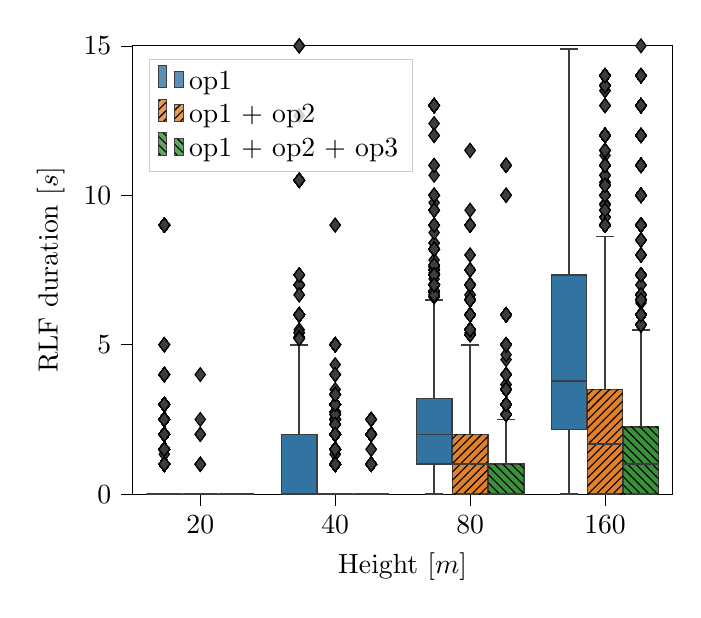
\begin{tikzpicture}

\definecolor{color0}{rgb}{0.194607843137255,0.453431372549019,0.632843137254902}
\definecolor{color1}{rgb}{0.881862745098039,0.505392156862745,0.173039215686275}
\definecolor{color2}{rgb}{0.229411764705882,0.570588235294118,0.229411764705882}

\begin{axis}[
legend cell align={left},
legend style={fill opacity=0.8, draw opacity=1, text opacity=1, at={(0.03,0.97)}, anchor=north west, draw=white!80!black},
tick align=outside,
tick pos=left,
x grid style={white!69.0196078431373!black},
xlabel={Height [$m$]},
xmin=-0.5, xmax=3.5,
xtick style={color=black},
xtick={0,1,2,3},
xticklabels={20,40,80,160},
y grid style={white!69.0196078431373!black},
ylabel={RLF duration [$s$]},
ymin=0, ymax=15,
ytick style={color=black}
]
\path [draw=white!23.921568627451!black, fill=color0, semithick]
(axis cs:-0.397333333333333,0)
--(axis cs:-0.136,0)
--(axis cs:-0.136,0)
--(axis cs:-0.397333333333333,0)
--(axis cs:-0.397333333333333,0)
--cycle;
\path [draw=white!23.921568627451!black, fill=color1, semithick][postaction={pattern=north east lines}]
(axis cs:-0.130666666666667,0)
--(axis cs:0.130666666666667,0)
--(axis cs:0.130666666666667,0)
--(axis cs:-0.130666666666667,0)
--(axis cs:-0.130666666666667,0)
--cycle;
\path [draw=white!23.921568627451!black, fill=color2, semithick][postaction={pattern=north west lines}]
(axis cs:0.136,0)
--(axis cs:0.397333333333333,0)
--(axis cs:0.397333333333333,0)
--(axis cs:0.136,0)
--(axis cs:0.136,0)
--cycle;
\path [draw=white!23.921568627451!black, fill=color0, semithick]
(axis cs:0.602666666666667,0)
--(axis cs:0.864,0)
--(axis cs:0.864,2)
--(axis cs:0.602666666666667,2)
--(axis cs:0.602666666666667,0)
--cycle;
\path [draw=white!23.921568627451!black, fill=color1, semithick][postaction={pattern=north east lines}]
(axis cs:0.869333333333333,0)
--(axis cs:1.13066666666667,0)
--(axis cs:1.13066666666667,0)
--(axis cs:0.869333333333333,0)
--(axis cs:0.869333333333333,0)
--cycle;
\path [draw=white!23.921568627451!black, fill=color2, semithick][postaction={pattern=north west lines}]
(axis cs:1.136,0)
--(axis cs:1.39733333333333,0)
--(axis cs:1.39733333333333,0)
--(axis cs:1.136,0)
--(axis cs:1.136,0)
--cycle;
\path [draw=white!23.921568627451!black, fill=color0, semithick]
(axis cs:1.60266666666667,1)
--(axis cs:1.864,1)
--(axis cs:1.864,3.2)
--(axis cs:1.60266666666667,3.2)
--(axis cs:1.60266666666667,1)
--cycle;
\path [draw=white!23.921568627451!black, fill=color1, semithick][postaction={pattern=north east lines}]
(axis cs:1.86933333333333,0)
--(axis cs:2.13066666666667,0)
--(axis cs:2.13066666666667,2)
--(axis cs:1.86933333333333,2)
--(axis cs:1.86933333333333,0)
--cycle;
\path [draw=white!23.921568627451!black, fill=color2, semithick][postaction={pattern=north west lines}]
(axis cs:2.136,0)
--(axis cs:2.39733333333333,0)
--(axis cs:2.39733333333333,1)
--(axis cs:2.136,1)
--(axis cs:2.136,0)
--cycle;
\path [draw=white!23.921568627451!black, fill=color0, semithick]
(axis cs:2.60266666666667,2.16666666666667)
--(axis cs:2.864,2.16666666666667)
--(axis cs:2.864,7.33333333333333)
--(axis cs:2.60266666666667,7.33333333333333)
--(axis cs:2.60266666666667,2.16666666666667)
--cycle;
\path [draw=white!23.921568627451!black, fill=color1, semithick][postaction={pattern=north east lines}]
(axis cs:2.86933333333333,0)
--(axis cs:3.13066666666667,0)
--(axis cs:3.13066666666667,3.5)
--(axis cs:2.86933333333333,3.5)
--(axis cs:2.86933333333333,0)
--cycle;
\path [draw=white!23.921568627451!black, fill=color2, semithick][postaction={pattern=north west lines}]
(axis cs:3.136,0)
--(axis cs:3.39733333333333,0)
--(axis cs:3.39733333333333,2.25)
--(axis cs:3.136,2.25)
--(axis cs:3.136,0)
--cycle;
\draw[draw=white!23.921568627451!black,fill=color0,line width=0.3pt] (axis cs:0,0) rectangle (axis cs:0,0);
\addlegendimage{ybar,ybar legend,draw=white!23.921568627451!black,fill=color0,line width=0.3pt};
\addlegendentry{op1}

\draw[draw=white!23.921568627451!black,fill=color1,line width=0.3pt] (axis cs:0,0) rectangle (axis cs:0,0);
\addlegendimage{ybar,ybar legend,draw=white!23.921568627451!black,fill=color1,line width=0.3pt,postaction={pattern=north east lines}};
\addlegendentry{op1 + op2}

\draw[draw=white!23.921568627451!black,fill=color2,line width=0.3pt] (axis cs:0,0) rectangle (axis cs:0,0);
\addlegendimage{ybar,ybar legend,draw=white!23.921568627451!black,fill=color2,line width=0.3pt,postaction={pattern=north west lines}};
\addlegendentry{op1 + op2 + op3}

\addplot [semithick, white!23.921568627451!black, forget plot]
table {%
-0.266666650772095 0
-0.266666650772095 0
};
\addplot [semithick, white!23.921568627451!black, forget plot]
table {%
-0.266666650772095 0
-0.266666650772095 0
};
\addplot [semithick, white!23.921568627451!black, forget plot]
table {%
-0.332000017166138 0
-0.201333284378052 0
};
\addplot [semithick, white!23.921568627451!black, forget plot]
table {%
-0.332000017166138 0
-0.201333284378052 0
};
\addplot [black, mark=diamond*, mark size=2.5, mark options={solid,fill=white!23.921568627451!black}, only marks, forget plot]
table {%
-0.266666650772095 1
-0.266666650772095 3
-0.266666650772095 1
-0.266666650772095 5
-0.266666650772095 4
-0.266666650772095 2
-0.266666650772095 1
-0.266666650772095 3
-0.266666650772095 1
-0.266666650772095 4
-0.266666650772095 2
-0.266666650772095 1
-0.266666650772095 3
-0.266666650772095 1
-0.266666650772095 4
-0.266666650772095 5
-0.266666650772095 1
-0.266666650772095 2
-0.266666650772095 4
-0.266666650772095 2.5
-0.266666650772095 1
-0.266666650772095 3
-0.266666650772095 1
-0.266666650772095 4
-0.266666650772095 5
-0.266666650772095 1
-0.266666650772095 2
-0.266666650772095 3
-0.266666650772095 1
-0.266666650772095 4
-0.266666650772095 3
-0.266666650772095 1
-0.266666650772095 1
-0.266666650772095 1
-0.266666650772095 3
-0.266666650772095 1
-0.266666650772095 5
-0.266666650772095 4
-0.266666650772095 3
-0.266666650772095 1
-0.266666650772095 2
-0.266666650772095 1
-0.266666650772095 4
-0.266666650772095 2.5
-0.266666650772095 1
-0.266666650772095 3
-0.266666650772095 1
-0.266666650772095 4
-0.266666650772095 5
-0.266666650772095 1
-0.266666650772095 2
-0.266666650772095 1
-0.266666650772095 3
-0.266666650772095 4
-0.266666650772095 2.5
-0.266666650772095 1
-0.266666650772095 3
-0.266666650772095 1
-0.266666650772095 5
-0.266666650772095 4
-0.266666650772095 2
-0.266666650772095 3
-0.266666650772095 1
-0.266666650772095 4
-0.266666650772095 2.5
-0.266666650772095 1
-0.266666650772095 3
-0.266666650772095 1
-0.266666650772095 4
-0.266666650772095 5
-0.266666650772095 1
-0.266666650772095 2
-0.266666650772095 3
-0.266666650772095 2.5
-0.266666650772095 4
-0.266666650772095 1
-0.266666650772095 3
-0.266666650772095 4
-0.266666650772095 1
-0.266666650772095 5
-0.266666650772095 1
-0.266666650772095 2
-0.266666650772095 3
-0.266666650772095 4
-0.266666650772095 2.5
-0.266666650772095 1
-0.266666650772095 3
-0.266666650772095 4
-0.266666650772095 5
-0.266666650772095 2
-0.266666650772095 1
-0.266666650772095 3
-0.266666650772095 4
-0.266666650772095 2.5
-0.266666650772095 1
-0.266666650772095 1
-0.266666650772095 3
-0.266666650772095 4
-0.266666650772095 5
-0.266666650772095 2
-0.266666650772095 1
-0.266666650772095 3
-0.266666650772095 1
-0.266666650772095 4
-0.266666650772095 2
-0.266666650772095 3
-0.266666650772095 1
-0.266666650772095 2.5
-0.266666650772095 3
-0.266666650772095 1
-0.266666650772095 1.5
-0.266666650772095 1
-0.266666650772095 2.5
-0.266666650772095 2
-0.266666650772095 1
-0.266666650772095 1.5
-0.266666650772095 1
-0.266666650772095 9
-0.266666650772095 1
-0.266666650772095 3
-0.266666650772095 2.5
-0.266666650772095 1.5
-0.266666650772095 3
-0.266666650772095 1
-0.266666650772095 1
-0.266666650772095 2.5
-0.266666650772095 2
-0.266666650772095 1
-0.266666650772095 9
-0.266666650772095 1.5
-0.266666650772095 1
-0.266666650772095 3
-0.266666650772095 2.5
-0.266666650772095 3
-0.266666650772095 1.5
-0.266666650772095 1
-0.266666650772095 2.5
-0.266666650772095 2
-0.266666650772095 1
-0.266666650772095 9
-0.266666650772095 1.5
-0.266666650772095 2
-0.266666650772095 1
-0.266666650772095 1
-0.266666650772095 1
-0.266666650772095 2.5
-0.266666650772095 1.5
-0.266666650772095 3
-0.266666650772095 1
-0.266666650772095 2.5
-0.266666650772095 2
-0.266666650772095 1
-0.266666650772095 9
-0.266666650772095 1.5
-0.266666650772095 1
-0.266666650772095 1
-0.266666650772095 3
-0.266666650772095 1
-0.266666650772095 2.5
-0.266666650772095 1.5
-0.266666650772095 3
-0.266666650772095 1
-0.266666650772095 2
-0.266666650772095 2.5
-0.266666650772095 1
-0.266666650772095 1
-0.266666650772095 9
-0.266666650772095 1.5
-0.266666650772095 2
-0.266666650772095 1
-0.266666650772095 3
-0.266666650772095 2.5
-0.266666650772095 1.5
-0.266666650772095 3
-0.266666650772095 1
-0.266666650772095 2.5
-0.266666650772095 2
-0.266666650772095 1
-0.266666650772095 1.5
-0.266666650772095 9
-0.266666650772095 1
-0.266666650772095 2
-0.266666650772095 1
-0.266666650772095 3
-0.266666650772095 2.5
-0.266666650772095 1.5
-0.266666650772095 3
-0.266666650772095 1
-0.266666650772095 2
-0.266666650772095 2.5
-0.266666650772095 1
-0.266666650772095 9
-0.266666650772095 1
-0.266666650772095 1.5
-0.266666650772095 2
-0.266666650772095 1
-0.266666650772095 2
-0.266666650772095 1
-0.266666650772095 3
-0.266666650772095 2.5
-0.266666650772095 1.5
-0.266666650772095 3
-0.266666650772095 1
-0.266666650772095 2
-0.266666650772095 2.5
-0.266666650772095 1
-0.266666650772095 1.5
-0.266666650772095 9
-0.266666650772095 1
-0.266666650772095 2
-0.266666650772095 1
-0.266666650772095 3
-0.266666650772095 2.5
-0.266666650772095 1.5
-0.266666650772095 3
-0.266666650772095 1
-0.266666650772095 2.5
-0.266666650772095 2
-0.266666650772095 1
-0.266666650772095 1.5
-0.266666650772095 9
-0.266666650772095 2
-0.266666650772095 1
-0.266666650772095 1
-0.266666650772095 2.5
-0.266666650772095 3
-0.266666650772095 1.5
-0.266666650772095 1
-0.266666650772095 2
-0.266666650772095 2.5
-0.266666650772095 1
-0.266666650772095 1.5
-0.266666650772095 9
-0.266666650772095 1
-0.266666650772095 1
-0.266666650772095 1
-0.266666650772095 3
-0.266666650772095 1
-0.266666650772095 2.5
-0.266666650772095 3
-0.266666650772095 1.5
-0.266666650772095 1
-0.266666650772095 2.5
-0.266666650772095 2
-0.266666650772095 1.5
-0.266666650772095 9
-0.266666650772095 2
-0.266666650772095 1
-0.266666650772095 3
-0.266666650772095 2.5
-0.266666650772095 3
-0.266666650772095 1
-0.266666650772095 1.5
-0.266666650772095 1
-0.266666650772095 2
-0.266666650772095 2.5
-0.266666650772095 1
-0.266666650772095 9
-0.266666650772095 1.5
-0.266666650772095 1
-0.266666650772095 2
-0.266666650772095 1
-0.266666650772095 3
-0.266666650772095 1
-0.266666650772095 2.5
-0.266666650772095 1.5
-0.266666650772095 3
-0.266666650772095 2.5
-0.266666650772095 2
-0.266666650772095 1
-0.266666650772095 9
-0.266666650772095 1.5
-0.266666650772095 2
-0.266666650772095 1
-0.266666650772095 3
-0.266666650772095 2.5
-0.266666650772095 1.5
-0.266666650772095 3
-0.266666650772095 1
-0.266666650772095 2
-0.266666650772095 2.5
-0.266666650772095 1
-0.266666650772095 1
-0.266666650772095 9
-0.266666650772095 2
-0.266666650772095 1
-0.266666650772095 3
-0.266666650772095 2.5
-0.266666650772095 3
-0.266666650772095 1
-0.266666650772095 1.5
-0.266666650772095 1
-0.266666650772095 2.5
-0.266666650772095 2
-0.266666650772095 1
-0.266666650772095 9
-0.266666650772095 1.5
-0.266666650772095 2
-0.266666650772095 1
-0.266666650772095 3
-0.266666650772095 1
-0.266666650772095 2.5
-0.266666650772095 1.5
-0.266666650772095 3
-0.266666650772095 1
-0.266666650772095 2
-0.266666650772095 2.5
-0.266666650772095 1
-0.266666650772095 9
-0.266666650772095 1.5
-0.266666650772095 1
-0.266666650772095 1
-0.266666650772095 3
-0.266666650772095 2.5
-0.266666650772095 3
-0.266666650772095 1.5
-0.266666650772095 1
-0.266666650772095 2.5
-0.266666650772095 2
-0.266666650772095 1
-0.266666650772095 1.5
-0.266666650772095 1
-0.266666650772095 9
-0.266666650772095 2
-0.266666650772095 1
-0.266666650772095 3
-0.266666650772095 2.5
-0.266666650772095 1.5
-0.266666650772095 1
-0.266666650772095 3
-0.266666650772095 1
-0.266666650772095 2.5
-0.266666650772095 2
-0.266666650772095 1
-0.266666650772095 1
-0.266666650772095 9
-0.266666650772095 1
-0.266666650772095 3
-0.266666650772095 1
-0.266666650772095 2.5
-0.266666650772095 1.5
-0.266666650772095 3
-0.266666650772095 1
-0.266666650772095 2
-0.266666650772095 2.5
-0.266666650772095 1
-0.266666650772095 1.5
-0.266666650772095 9
-0.266666650772095 1
-0.266666650772095 2
-0.266666650772095 1
-0.266666650772095 3
-0.266666650772095 2.5
-0.266666650772095 3
-0.266666650772095 1
-0.266666650772095 1.5
-0.266666650772095 1
-0.266666650772095 2.5
-0.266666650772095 2
-0.266666650772095 1
-0.266666650772095 9
-0.266666650772095 1
-0.266666650772095 1
-0.266666650772095 3
-0.266666650772095 2.5
-0.266666650772095 1.5
-0.266666650772095 1
-0.266666650772095 3
-0.266666650772095 1
-0.266666650772095 2
-0.266666650772095 2.5
-0.266666650772095 1
-0.266666650772095 1.5
-0.266666650772095 9
-0.266666650772095 2
-0.266666650772095 1
-0.266666650772095 3
-0.266666650772095 2.5
-0.266666650772095 1
-0.266666650772095 3
-0.266666650772095 1.5
-0.266666650772095 1
-0.266666650772095 2.5
-0.266666650772095 2
-0.266666650772095 1
-0.266666650772095 9
-0.266666650772095 1
-0.266666650772095 1.5
-0.266666650772095 2
-0.266666650772095 1
-0.266666650772095 3
-0.266666650772095 1
-0.266666650772095 2.5
-0.266666650772095 1.5
-0.266666650772095 3
-0.266666650772095 1
-0.266666650772095 2
-0.266666650772095 2.5
-0.266666650772095 1
-0.266666650772095 9
-0.266666650772095 1
-0.266666650772095 2
-0.266666650772095 1
-0.266666650772095 3
-0.266666650772095 2.5
-0.266666650772095 1
-0.266666650772095 3
-0.266666650772095 1.5
-0.266666650772095 1
-0.266666650772095 2
-0.266666650772095 2.5
-0.266666650772095 1
-0.266666650772095 1.5
-0.266666650772095 9
-0.266666650772095 1
-0.266666650772095 3
-0.266666650772095 1
-0.266666650772095 2.5
-0.266666650772095 3
-0.266666650772095 1.5
-0.266666650772095 1
-0.266666650772095 2
-0.266666650772095 1
-0.266666650772095 2.5
-0.266666650772095 1
-0.266666650772095 9
-0.266666650772095 2
-0.266666650772095 1
-0.266666650772095 3
-0.266666650772095 1
-0.266666650772095 2.5
-0.266666650772095 1.5
-0.266666650772095 1
-0.266666650772095 3
-0.266666650772095 1
-0.266666650772095 2.5
-0.266666650772095 2
-0.266666650772095 1
-0.266666650772095 9
-0.266666650772095 1.5
-0.266666650772095 1
-0.266666650772095 3
-0.266666650772095 1
-0.266666650772095 2.5
-0.266666650772095 3
-0.266666650772095 1.5
-0.266666650772095 1
-0.266666650772095 2.5
-0.266666650772095 1
-0.266666650772095 2
-0.266666650772095 1
-0.266666650772095 1.5
-0.266666650772095 1
-0.266666650772095 9
-0.266666650772095 1
-0.266666650772095 1
-0.266666650772095 3
-0.266666650772095 2.5
-0.266666650772095 3
-0.266666650772095 1.5
-0.266666650772095 1
-0.266666650772095 2
-0.266666650772095 2.5
-0.266666650772095 1
-0.266666650772095 1.5
-0.266666650772095 9
-0.266666650772095 2
-0.266666650772095 1
-0.266666650772095 3
-0.266666650772095 1.5
-0.266666650772095 2.5
-0.266666650772095 3
-0.266666650772095 1
-0.266666650772095 2
-0.266666650772095 2.5
-0.266666650772095 1
-0.266666650772095 1.5
-0.266666650772095 9
-0.266666650772095 2
-0.266666650772095 1
-0.266666650772095 3
-0.266666650772095 2.5
-0.266666650772095 3
-0.266666650772095 1.5
-0.266666650772095 2.5
-0.266666650772095 2
-0.266666650772095 1
-0.266666650772095 9
-0.266666650772095 1
-0.266666650772095 2
-0.266666650772095 1
-0.266666650772095 3
-0.266666650772095 2.5
-0.266666650772095 3
-0.266666650772095 1.5
-0.266666650772095 1
-0.266666650772095 2
-0.266666650772095 2.5
-0.266666650772095 1
-0.266666650772095 9
-0.266666650772095 1
-0.266666650772095 2
-0.266666650772095 1
-0.266666650772095 3
-0.266666650772095 2.5
-0.266666650772095 1.5
-0.266666650772095 3
-0.266666650772095 1
-0.266666650772095 2
-0.266666650772095 2.5
-0.266666650772095 1.5
-0.266666650772095 1
-0.266666650772095 9
-0.266666650772095 1
-0.266666650772095 2
-0.266666650772095 1
-0.266666650772095 3
-0.266666650772095 1
-0.266666650772095 2.5
-0.266666650772095 3
-0.266666650772095 1.5
-0.266666650772095 2.5
-0.266666650772095 1
-0.266666650772095 1.5
-0.266666650772095 9
-0.266666650772095 1
-0.266666650772095 2
-0.266666650772095 1
-0.266666650772095 3
-0.266666650772095 1
-0.266666650772095 1.5
-0.266666650772095 1
-0.266666650772095 2
-0.266666650772095 1
-0.266666650772095 2.5
-0.266666650772095 1
-0.266666650772095 1.5
-0.266666650772095 1
-0.266666650772095 9
-0.266666650772095 2
-0.266666650772095 1
-0.266666650772095 1
-0.266666650772095 3
-0.266666650772095 2.5
-0.266666650772095 1.5
-0.266666650772095 3
-0.266666650772095 1
-0.266666650772095 2
-0.266666650772095 2.5
-0.266666650772095 1
-0.266666650772095 9
-0.266666650772095 1.5
-0.266666650772095 1
-0.266666650772095 2.5
-0.266666650772095 1
-0.266666650772095 3
-0.266666650772095 2.5
-0.266666650772095 3
-0.266666650772095 1.5
-0.266666650772095 1
-0.266666650772095 2.5
-0.266666650772095 2
-0.266666650772095 1
-0.266666650772095 9
-0.266666650772095 1.5
-0.266666650772095 2
-0.266666650772095 1
-0.266666650772095 3
-0.266666650772095 4
-0.266666650772095 1
-0.266666650772095 1.5
-0.266666650772095 1
-0.266666650772095 3
-0.266666650772095 1
-0.266666650772095 2
-0.266666650772095 2.5
-0.266666650772095 1
-0.266666650772095 2
-0.266666650772095 1.5
-0.266666650772095 9
-0.266666650772095 1.33333337306976
-0.266666650772095 1
-0.266666650772095 3
-0.266666650772095 2.5
-0.266666650772095 3
-0.266666650772095 1
-0.266666650772095 1.5
-0.266666650772095 1
-0.266666650772095 2
-0.266666650772095 2.5
-0.266666650772095 1
-0.266666650772095 9
-0.266666650772095 1.5
-0.266666650772095 2
-0.266666650772095 1
-0.266666650772095 3
-0.266666650772095 1
-0.266666650772095 2.5
-0.266666650772095 3
-0.266666650772095 1.5
-0.266666650772095 1
-0.266666650772095 2.5
-0.266666650772095 1
-0.266666650772095 2
-0.266666650772095 1
-0.266666650772095 9
-0.266666650772095 1.5
-0.266666650772095 2
-0.266666650772095 1
-0.266666650772095 3
-0.266666650772095 2.5
-0.266666650772095 3
-0.266666650772095 1
-0.266666650772095 1.5
-0.266666650772095 1
-0.266666650772095 2
-0.266666650772095 2.5
-0.266666650772095 1
-0.266666650772095 1.5
-0.266666650772095 9
};
\addplot [semithick, white!23.921568627451!black, forget plot]
table {%
0 0
0 0
};
\addplot [semithick, white!23.921568627451!black, forget plot]
table {%
0 0
0 0
};
\addplot [semithick, white!23.921568627451!black, forget plot]
table {%
-0.065333366394043 0
0.065333366394043 0
};
\addplot [semithick, white!23.921568627451!black, forget plot]
table {%
-0.065333366394043 0
0.065333366394043 0
};
\addplot [black, mark=diamond*, mark size=2.5, mark options={solid,fill=white!23.921568627451!black}, only marks, forget plot]
table {%
0 4
0 1
0 2
0 1
0 2
0 1
0 2.5
0 2
0 1
0 1
};
\addplot [semithick, white!23.921568627451!black, forget plot]
table {%
0.266666650772095 0
0.266666650772095 0
};
\addplot [semithick, white!23.921568627451!black, forget plot]
table {%
0.266666650772095 0
0.266666650772095 0
};
\addplot [semithick, white!23.921568627451!black, forget plot]
table {%
0.201333284378052 0
0.332000017166138 0
};
\addplot [semithick, white!23.921568627451!black, forget plot]
table {%
0.201333284378052 0
0.332000017166138 0
};
\addplot [semithick, white!23.921568627451!black, forget plot]
table {%
0.733333349227905 0
0.733333349227905 0
};
\addplot [semithick, white!23.921568627451!black, forget plot]
table {%
0.733333349227905 2
0.733333349227905 5
};
\addplot [semithick, white!23.921568627451!black, forget plot]
table {%
0.667999982833862 0
0.798666715621948 0
};
\addplot [semithick, white!23.921568627451!black, forget plot]
table {%
0.667999982833862 5
0.798666715621948 5
};
\addplot [black, mark=diamond*, mark size=2.5, mark options={solid,fill=white!23.921568627451!black}, only marks, forget plot]
table {%
0.733333349227905 7
0.733333349227905 6
0.733333349227905 7
0.733333349227905 6
0.733333349227905 7
0.733333349227905 6
0.733333349227905 7
0.733333349227905 12.6666669845581
0.733333349227905 6
0.733333349227905 7
0.733333349227905 6
0.733333349227905 7
0.733333349227905 6
0.733333349227905 7
0.733333349227905 6
0.733333349227905 7
0.733333349227905 6
0.733333349227905 10.5
0.733333349227905 6
0.733333349227905 10.5
0.733333349227905 6
0.733333349227905 10.5
0.733333349227905 6
0.733333349227905 10.5
0.733333349227905 10.5
0.733333349227905 6
0.733333349227905 6
0.733333349227905 10.5
0.733333349227905 5.40000009536743
0.733333349227905 6
0.733333349227905 10.5
0.733333349227905 6
0.733333349227905 10.5
0.733333349227905 6
0.733333349227905 10.5
0.733333349227905 6
0.733333349227905 10.5
0.733333349227905 6
0.733333349227905 10.5
0.733333349227905 5.40000009536743
0.733333349227905 10.5
0.733333349227905 6
0.733333349227905 22
0.733333349227905 7.33333349227905
0.733333349227905 5.25
0.733333349227905 6
0.733333349227905 10.5
0.733333349227905 6
0.733333349227905 10.5
0.733333349227905 6
0.733333349227905 10.5
0.733333349227905 6
0.733333349227905 15
0.733333349227905 5.5
0.733333349227905 6.66666650772095
0.733333349227905 7.33333349227905
0.733333349227905 22
0.733333349227905 6
0.733333349227905 10.5
0.733333349227905 6
0.733333349227905 22
0.733333349227905 6.66666650772095
0.733333349227905 7.33333349227905
0.733333349227905 6
0.733333349227905 10.5
0.733333349227905 6
0.733333349227905 10.5
0.733333349227905 6
0.733333349227905 22
0.733333349227905 5.25
0.733333349227905 7.33333349227905
0.733333349227905 6
0.733333349227905 10.5
0.733333349227905 6
0.733333349227905 15
0.733333349227905 7.33333349227905
0.733333349227905 5.25
0.733333349227905 6
0.733333349227905 15
0.733333349227905 10.5
0.733333349227905 6
0.733333349227905 5.40000009536743
0.733333349227905 10.5
0.733333349227905 6
0.733333349227905 10.5
0.733333349227905 6
0.733333349227905 10.5
0.733333349227905 6
0.733333349227905 15
0.733333349227905 7.33333349227905
0.733333349227905 5.25
0.733333349227905 6
0.733333349227905 5.19999980926514
0.733333349227905 22
0.733333349227905 5.25
0.733333349227905 6
0.733333349227905 10.5
0.733333349227905 6
0.733333349227905 10.5
0.733333349227905 5.19999980926514
0.733333349227905 6
0.733333349227905 10.5
0.733333349227905 6
0.733333349227905 10.5
0.733333349227905 6
0.733333349227905 10.5
0.733333349227905 6
0.733333349227905 10.5
};
\addplot [semithick, white!23.921568627451!black, forget plot]
table {%
1 0
1 0
};
\addplot [semithick, white!23.921568627451!black, forget plot]
table {%
1 0
1 0
};
\addplot [semithick, white!23.921568627451!black, forget plot]
table {%
0.934666633605957 0
1.06533336639404 0
};
\addplot [semithick, white!23.921568627451!black, forget plot]
table {%
0.934666633605957 0
1.06533336639404 0
};
\addplot [black, mark=diamond*, mark size=2.5, mark options={solid,fill=white!23.921568627451!black}, only marks, forget plot]
table {%
1 2
1 2
1 4
1 1
1 1.5
1 3
1 2
1 3
1 1
1 2
1 1.5
1 2.5
1 1
1 1.5
1 1
1 3
1 2
1 3
1 1
1 2
1 1.5
1 2.5
1 1
1 1.5
1 1
1 3
1 1
1 3
1 2
1 1.5
1 1
1 1
1 1.33333337306976
1 1
1 5
1 1
1 3
1 1
1 2
1 2
1 1.5
1 3.5
1 2
1 1
1 1.33333337306976
1 1
1 5
1 1
1 3
1 1
1 2
1 1.5
1 2.5
1 1
1 1.5
1 1
1 3
1 2
1 3
1 1
1 2
1 2
1 1.5
1 2.5
1 1
1 1.5
1 1
1 3
1 3
1 1
1 2
1 1.5
1 2.5
1 1
1 1.5
1 1
1 3
1 2
1 3
1 1
1 2
1 1.5
1 2.5
1 1
1 1.5
1 1
1 3
1 2
1 3
1 1
1 1
1 2
1 2.5
1 1
1 1.5
1 3
1 1
1 2
1 1
1 3
1 1
1 2
1 3.33333325386047
1 1.5
1 5
1 1
1 3
1 1
1 2
1 3.33333325386047
1 1
1 1.5
1 5
1 1
1 1
1 2
1 3
1 1
1 2
1 2.66666674613953
1 1.5
1 5
1 1
1 3
1 1
1 2
1 3.33333325386047
1 1.5
1 5
1 1
1 3
1 1
1 2
1 3.33333325386047
1 1.5
1 5
1 1
1 3
1 1
1 2
1 2.66666674613953
1 1.5
1 5
1 1
1 2
1 3
1 1
1 2
1 3.33333325386047
1 1
1 2
1 5
1 1
1 1
1 3
1 1
1 1
1 2
1 2.66666674613953
1 1
1 1.5
1 5
1 1
1 1
1 2
1 3
1 1
1 2
1 1
1 1.5
1 3
1 1
1 4
1 3
1 2
1 3
1 1
1 1
1 2
1 3.33333325386047
1 1
1 1.5
1 5
1 1
1 1
1 2
1 3
1 1
1 2
1 2.33333325386047
1 1
1 1.5
1 4
1 1
1 3
1 1
1 2
1 3.33333325386047
1 1.5
1 5
1 1
1 2
1 3
1 1
1 2
1 2.33333325386047
1 1
1 3
1 5
1 1
1 2
1 3
1 1
1 2
1 2.33333325386047
1 1
1 2.5
1 1.5
1 5
1 2.75
1 1
1 2
1 3
1 1
1 2
1 2.33333325386047
1 1
1 1.5
1 1
1 3
1 1
1 2
1 3.33333325386047
1 1
1 1.5
1 5
1 1
1 3
1 1
1 2
1 2.66666674613953
1 1
1 1.5
1 5
1 1
1 3
1 1
1 2
1 3.33333325386047
1 2.5
1 1.5
1 9
1 2.75
1 1
1 2
1 3
1 1
1 2
1 2.66666674613953
1 1.5
1 5
1 1
1 3
1 1
1 2
1 3.33333325386047
1 1
1 2.5
1 1.5
1 5
1 2.75
1 1
1 2
1 3
1 1
1 2
1 2.33333325386047
1 1
1 1.5
1 5
1 1
1 1
1 2
1 1
1 1.5
1 4
1 1
1 1
1 3
1 1
1 2
1 3
1 1
1 2.5
1 1.5
1 5
1 2.75
1 1
1 3
1 1
1 2
1 4.33333349227905
1 1.5
1 5
1 1
1 3
1 2
1 2
1 1
1 2.5
1 1.5
1 5
1 2.5
1 1
1 3
1 1
1 2
1 3.33333325386047
1 1
1 1.5
1 9
1 1
1 3
1 1
1 2
1 3.33333325386047
1 1
1 1.5
1 4
1 1
1 1
1 1
1 2
1 1.5
1 5
1 1
1 2
1 3
1 1
1 2
1 1.5
1 5
1 1
1 1
1 2
1 3
1 1
1 2
1 1
1 2.5
1 1.5
1 5
1 2.5
1 1
1 2
1 3
1 1
1 2
1 2.66666674613953
1 1
1 2.5
1 1.5
1 5
1 2.75
1 1
1 2
1 3
1 1
1 1
1 2
1 2.33333325386047
1 1
1 1.5
1 4
1 1
1 1
1 3
1 1
1 2
1 2.33333325386047
1 1
1 1.5
1 5
1 1
1 3
1 1
1 2
1 3
1 1.5
1 5
1 1
1 3
1 1
1 2
1 1.5
1 5
1 1
1 3
1 1
1 1
1 2
1 1
1 1.5
1 5
1 1
1 2
1 3
1 1
1 2
1 2.66666674613953
1 1.5
1 5
1 1
1 1
1 2
1 3
1 1
1 1
1 2
1 2.33333325386047
1 1
1 5
1 1
1 3
1 1
1 2
1 2.33333325386047
1 1
1 1.5
1 5
1 1
1 2
1 3
1 1
1 2
1 3.33333325386047
1 1
1 1.5
1 5
1 1
};
\addplot [semithick, white!23.921568627451!black, forget plot]
table {%
1.26666665077209 0
1.26666665077209 0
};
\addplot [semithick, white!23.921568627451!black, forget plot]
table {%
1.26666665077209 0
1.26666665077209 0
};
\addplot [semithick, white!23.921568627451!black, forget plot]
table {%
1.20133328437805 0
1.33200001716614 0
};
\addplot [semithick, white!23.921568627451!black, forget plot]
table {%
1.20133328437805 0
1.33200001716614 0
};
\addplot [black, mark=diamond*, mark size=2.5, mark options={solid,fill=white!23.921568627451!black}, only marks, forget plot]
table {%
1.26666665077209 2
1.26666665077209 1
1.26666665077209 2
1.26666665077209 1
1.26666665077209 2
1.26666665077209 1
1.26666665077209 2
1.26666665077209 1.5
1.26666665077209 1
1.26666665077209 2
1.26666665077209 1.5
1.26666665077209 1
1.26666665077209 2
1.26666665077209 1
1.26666665077209 2
1.26666665077209 1
1.26666665077209 2
1.26666665077209 2
1.26666665077209 1
1.26666665077209 2
1.26666665077209 1
1.26666665077209 2
1.26666665077209 1
1.26666665077209 2
1.26666665077209 1
1.26666665077209 2
1.26666665077209 1
1.26666665077209 2
1.26666665077209 1
1.26666665077209 2
1.26666665077209 1
1.26666665077209 2
1.26666665077209 2
1.26666665077209 1
1.26666665077209 2
1.26666665077209 1
1.26666665077209 2
1.26666665077209 1
1.26666665077209 2
1.26666665077209 1
1.26666665077209 2
1.26666665077209 1
1.26666665077209 2
1.26666665077209 1
1.26666665077209 1
1.26666665077209 2
1.26666665077209 1
1.26666665077209 2
1.26666665077209 1
1.26666665077209 2
1.26666665077209 1
1.26666665077209 2.5
1.26666665077209 1
1.26666665077209 2
1.26666665077209 2.5
1.26666665077209 1
1.26666665077209 2
1.26666665077209 1
1.26666665077209 2
1.26666665077209 2
1.26666665077209 2
1.26666665077209 2.5
1.26666665077209 1
1.26666665077209 2
1.26666665077209 1
1.26666665077209 2
1.26666665077209 2.5
1.26666665077209 1
1.26666665077209 2
1.26666665077209 1
1.26666665077209 2
1.26666665077209 1
1.26666665077209 1
1.26666665077209 2
1.26666665077209 2.5
1.26666665077209 1
1.26666665077209 2
1.26666665077209 1
1.26666665077209 2
1.26666665077209 2.5
1.26666665077209 1
1.26666665077209 2
1.26666665077209 2
1.26666665077209 1
1.26666665077209 2
1.26666665077209 1
1.26666665077209 2
1.26666665077209 1
1.26666665077209 2
1.26666665077209 1
1.26666665077209 1
1.26666665077209 2
1.26666665077209 1
1.26666665077209 2.5
1.26666665077209 1
1.26666665077209 2
1.26666665077209 1
1.26666665077209 2.5
1.26666665077209 1
1.26666665077209 2
1.26666665077209 1
1.26666665077209 2
1.26666665077209 1
1.26666665077209 2
1.26666665077209 1
1.26666665077209 1
1.26666665077209 2
1.26666665077209 1
1.26666665077209 2
1.26666665077209 1
1.26666665077209 2
1.26666665077209 1
1.26666665077209 2
1.26666665077209 1
1.26666665077209 2.5
1.26666665077209 1
1.26666665077209 2
1.26666665077209 1
1.26666665077209 2
1.26666665077209 1
1.26666665077209 1
};
\addplot [semithick, white!23.921568627451!black, forget plot]
table {%
1.73333334922791 1
1.73333334922791 0
};
\addplot [semithick, white!23.921568627451!black, forget plot]
table {%
1.73333334922791 3.20000004768372
1.73333334922791 6.5
};
\addplot [semithick, white!23.921568627451!black, forget plot]
table {%
1.66799998283386 0
1.79866671562195 0
};
\addplot [semithick, white!23.921568627451!black, forget plot]
table {%
1.66799998283386 6.5
1.79866671562195 6.5
};
\addplot [black, mark=diamond*, mark size=2.5, mark options={solid,fill=white!23.921568627451!black}, only marks, forget plot]
table {%
1.73333334922791 17
1.73333334922791 9
1.73333334922791 20
1.73333334922791 7.5
1.73333334922791 9.5
1.73333334922791 7.33333349227905
1.73333334922791 6.80000019073486
1.73333334922791 6.75
1.73333334922791 17
1.73333334922791 7.5
1.73333334922791 7
1.73333334922791 7.5
1.73333334922791 20
1.73333334922791 7.33333349227905
1.73333334922791 17
1.73333334922791 7.66666650772095
1.73333334922791 20
1.73333334922791 10
1.73333334922791 7.33333349227905
1.73333334922791 7.40000009536743
1.73333334922791 17
1.73333334922791 28
1.73333334922791 7.5
1.73333334922791 7
1.73333334922791 7.33333349227905
1.73333334922791 6.75
1.73333334922791 9
1.73333334922791 17
1.73333334922791 7
1.73333334922791 7.19999980926514
1.73333334922791 9
1.73333334922791 6.80000019073486
1.73333334922791 7
1.73333334922791 12.3999996185303
1.73333334922791 7.5
1.73333334922791 7.83333349227905
1.73333334922791 17
1.73333334922791 9
1.73333334922791 7
1.73333334922791 7.5
1.73333334922791 20
1.73333334922791 7.59999990463257
1.73333334922791 20
1.73333334922791 6.59999990463257
1.73333334922791 17
1.73333334922791 6.75
1.73333334922791 7
1.73333334922791 7.5
1.73333334922791 20
1.73333334922791 7.33333349227905
1.73333334922791 17
1.73333334922791 9
1.73333334922791 20
1.73333334922791 9.75
1.73333334922791 7.33333349227905
1.73333334922791 7
1.73333334922791 6.59999990463257
1.73333334922791 9
1.73333334922791 7.5
1.73333334922791 7.59999990463257
1.73333334922791 9.5
1.73333334922791 6.59999990463257
1.73333334922791 17
1.73333334922791 7.5
1.73333334922791 7
1.73333334922791 7.5
1.73333334922791 20
1.73333334922791 9.5
1.73333334922791 7
1.73333334922791 13
1.73333334922791 9.5
1.73333334922791 7
1.73333334922791 13
1.73333334922791 8.19999980926514
1.73333334922791 9.5
1.73333334922791 7
1.73333334922791 13
1.73333334922791 8.19999980926514
1.73333334922791 20
1.73333334922791 7
1.73333334922791 13
1.73333334922791 8.19999980926514
1.73333334922791 20
1.73333334922791 13
1.73333334922791 8.19999980926514
1.73333334922791 20
1.73333334922791 7
1.73333334922791 13
1.73333334922791 8.19999980926514
1.73333334922791 7.33333349227905
1.73333334922791 7
1.73333334922791 9
1.73333334922791 13
1.73333334922791 8.19999980926514
1.73333334922791 7.33333349227905
1.73333334922791 7
1.73333334922791 13
1.73333334922791 7
1.73333334922791 7.33333349227905
1.73333334922791 7
1.73333334922791 13
1.73333334922791 8.19999980926514
1.73333334922791 7.33333349227905
1.73333334922791 7
1.73333334922791 12
1.73333334922791 10
1.73333334922791 7.33333349227905
1.73333334922791 7
1.73333334922791 13
1.73333334922791 8.19999980926514
1.73333334922791 7.33333349227905
1.73333334922791 7
1.73333334922791 9
1.73333334922791 9
1.73333334922791 7
1.73333334922791 7.66666650772095
1.73333334922791 11
1.73333334922791 7
1.73333334922791 9.5
1.73333334922791 7
1.73333334922791 7.33333349227905
1.73333334922791 7
1.73333334922791 13
1.73333334922791 8.19999980926514
1.73333334922791 7.33333349227905
1.73333334922791 13
1.73333334922791 8.19999980926514
1.73333334922791 7.33333349227905
1.73333334922791 7
1.73333334922791 13
1.73333334922791 8.19999980926514
1.73333334922791 7
1.73333334922791 8.39999961853027
1.73333334922791 10.6666669845581
1.73333334922791 7
1.73333334922791 20
1.73333334922791 7
1.73333334922791 13
1.73333334922791 11
1.73333334922791 7
1.73333334922791 7
1.73333334922791 9.5
1.73333334922791 7
1.73333334922791 7.33333349227905
1.73333334922791 7
1.73333334922791 13
1.73333334922791 7.33333349227905
1.73333334922791 7
1.73333334922791 10
1.73333334922791 8.39999961853027
1.73333334922791 6.80000019073486
1.73333334922791 7.66666650772095
1.73333334922791 9.5
1.73333334922791 7
1.73333334922791 20
1.73333334922791 7
1.73333334922791 13
1.73333334922791 8.19999980926514
1.73333334922791 6.80000019073486
1.73333334922791 7
1.73333334922791 6.66666650772095
1.73333334922791 7.33333349227905
1.73333334922791 7
1.73333334922791 12
1.73333334922791 20
1.73333334922791 7
1.73333334922791 10
1.73333334922791 7.33333349227905
1.73333334922791 7
1.73333334922791 13
1.73333334922791 6.75
1.73333334922791 8.19999980926514
1.73333334922791 10
1.73333334922791 20
1.73333334922791 7
1.73333334922791 13
1.73333334922791 8.19999980926514
1.73333334922791 6.80000019073486
1.73333334922791 7
1.73333334922791 7
1.73333334922791 6.66666650772095
1.73333334922791 11
1.73333334922791 8.75
1.73333334922791 8.19999980926514
1.73333334922791 7
1.73333334922791 9.5
1.73333334922791 10
1.73333334922791 7.33333349227905
1.73333334922791 7
1.73333334922791 12
1.73333334922791 10
1.73333334922791 20
1.73333334922791 7
1.73333334922791 13
1.73333334922791 8.19999980926514
1.73333334922791 9.5
1.73333334922791 7
1.73333334922791 9
1.73333334922791 13
1.73333334922791 8.19999980926514
1.73333334922791 7.33333349227905
1.73333334922791 7
1.73333334922791 13
1.73333334922791 8.19999980926514
1.73333334922791 7.33333349227905
1.73333334922791 7
1.73333334922791 13
1.73333334922791 8.19999980926514
1.73333334922791 20
1.73333334922791 13
1.73333334922791 8.19999980926514
1.73333334922791 7.33333349227905
1.73333334922791 7
1.73333334922791 9
1.73333334922791 13
1.73333334922791 8.19999980926514
1.73333334922791 7.33333349227905
1.73333334922791 7
1.73333334922791 13
1.73333334922791 8.19999980926514
1.73333334922791 7.33333349227905
1.73333334922791 7
1.73333334922791 13
1.73333334922791 8.19999980926514
};
\addplot [semithick, white!23.921568627451!black, forget plot]
table {%
2 0
2 0
};
\addplot [semithick, white!23.921568627451!black, forget plot]
table {%
2 2
2 5
};
\addplot [semithick, white!23.921568627451!black, forget plot]
table {%
1.93466663360596 0
2.06533336639404 0
};
\addplot [semithick, white!23.921568627451!black, forget plot]
table {%
1.93466663360596 5
2.06533336639404 5
};
\addplot [black, mark=diamond*, mark size=2.5, mark options={solid,fill=white!23.921568627451!black}, only marks, forget plot]
table {%
2 5.40000009536743
2 17
2 6.5
2 7.5
2 9
2 17
2 5.5
2 6
2 6.5
2 9
2 17
2 6
2 5.5
2 6.5
2 9
2 17
2 5.33333349227905
2 5.5
2 6.5
2 7.5
2 9
2 17
2 8
2 9.5
2 6
2 6.5
2 7.5
2 9
2 17
2 6
2 7
2 5.5
2 6
2 6.5
2 7.5
2 9
2 17
2 7
2 5.5
2 6.5
2 9
2 17
2 6
2 5.5
2 6.5
2 7.5
2 9
2 17
2 6
2 7
2 5.5
2 6
2 7.5
2 9
2 17
2 7
2 5.5
2 6
2 6.5
2 7
2 5.5
2 5.33333349227905
2 7
2 5.5
2 6
2 5.5
2 6.5
2 7
2 5.5
2 6
2 5.33333349227905
2 7
2 5.5
2 6
2 6.5
2 8
2 7
2 5.5
2 6
2 6.5
2 7
2 5.5
2 6
2 5.33333349227905
2 6.5
2 7
2 5.5
2 6.5
2 5.5
2 6
2 6.5
2 6
2 6.5
2 6
2 6.5
2 22
2 5.5
2 6
2 6.5
2 7
2 5.5
2 6
2 7
2 5.5
2 6.5
2 5.5
2 6
2 6.5
2 11.5
2 5.5
2 6.5
2 7
2 6.5
2 22
2 5.5
2 6.5
2 7
2 5.5
2 6
2 6.5
2 5.5
2 6
2 11.5
2 5.5
2 6
2 6.5
2 7
2 5.5
2 5.33333349227905
2 6.5
2 6.66666650772095
2 5.5
2 6
2 7
2 5.5
2 5.33333349227905
2 6.5
2 7
2 5.5
2 6.5
2 5.5
2 6.5
2 5.5
2 6
2 6.5
2 6.66666650772095
2 5.5
2 6
2 6.5
2 22
2 5.5
2 6
2 5.5
2 6.5
2 7
2 5.5
2 6
2 6.5
2 6
2 6.5
2 7
2 5.5
2 6
2 5.5
2 6.5
2 7
2 5.5
2 6.5
2 7
2 5.5
2 6
2 6.5
2 7
2 6
2 6.5
2 5.5
2 6
2 6.5
2 7
2 5.5
2 6.5
};
\addplot [semithick, white!23.921568627451!black, forget plot]
table {%
2.26666665077209 0
2.26666665077209 0
};
\addplot [semithick, white!23.921568627451!black, forget plot]
table {%
2.26666665077209 1
2.26666665077209 2.5
};
\addplot [semithick, white!23.921568627451!black, forget plot]
table {%
2.20133328437805 0
2.33200001716614 0
};
\addplot [semithick, white!23.921568627451!black, forget plot]
table {%
2.20133328437805 2.5
2.33200001716614 2.5
};
\addplot [black, mark=diamond*, mark size=2.5, mark options={solid,fill=white!23.921568627451!black}, only marks, forget plot]
table {%
2.26666665077209 3
2.26666665077209 3
2.26666665077209 4
2.26666665077209 4.5
2.26666665077209 6
2.26666665077209 5
2.26666665077209 3
2.26666665077209 6
2.26666665077209 3
2.26666665077209 3.5
2.26666665077209 3
2.26666665077209 4
2.26666665077209 2.66666674613953
2.26666665077209 10
2.26666665077209 6
2.26666665077209 3
2.26666665077209 5
2.26666665077209 3
2.26666665077209 3.5
2.26666665077209 3
2.26666665077209 4
2.26666665077209 6
2.26666665077209 3.66666674613953
2.26666665077209 3.5
2.26666665077209 3.5
2.26666665077209 3
2.26666665077209 4.66666650772095
2.26666665077209 11
2.26666665077209 3
2.26666665077209 4
2.26666665077209 3
2.26666665077209 3
2.26666665077209 10
2.26666665077209 6
2.26666665077209 5
2.26666665077209 3.5
2.26666665077209 3
2.26666665077209 2.66666674613953
2.26666665077209 6
2.26666665077209 3
2.26666665077209 3.5
2.26666665077209 3
2.26666665077209 4
2.26666665077209 10
2.26666665077209 6
2.26666665077209 5
2.26666665077209 3
2.26666665077209 3.5
2.26666665077209 3
2.26666665077209 3
2.26666665077209 10
2.26666665077209 6
2.26666665077209 5
2.26666665077209 3.5
2.26666665077209 3
2.26666665077209 3
2.26666665077209 6
2.26666665077209 3.5
2.26666665077209 6
2.26666665077209 5
2.26666665077209 3.5
2.26666665077209 2.66666674613953
2.26666665077209 3.5
2.26666665077209 6
2.26666665077209 3.5
2.26666665077209 3
2.26666665077209 3
2.26666665077209 3.5
2.26666665077209 2.66666674613953
2.26666665077209 6
2.26666665077209 3.5
2.26666665077209 3
2.26666665077209 3.5
2.26666665077209 3
2.26666665077209 6
2.26666665077209 5
2.26666665077209 3.5
2.26666665077209 2.66666674613953
2.26666665077209 3
2.26666665077209 3.5
2.26666665077209 6
2.26666665077209 3
2.26666665077209 3.5
2.26666665077209 3
2.26666665077209 6
2.26666665077209 5
2.26666665077209 3.5
2.26666665077209 3
2.26666665077209 3.5
2.26666665077209 3
2.26666665077209 3
2.26666665077209 6
2.26666665077209 3
2.26666665077209 3.5
2.26666665077209 3
2.26666665077209 6
2.26666665077209 3
2.26666665077209 3.5
2.26666665077209 3.5
2.26666665077209 6
2.26666665077209 3
2.26666665077209 3.5
2.26666665077209 3
2.26666665077209 3.5
2.26666665077209 3
2.26666665077209 6
2.26666665077209 3.5
2.26666665077209 3
2.26666665077209 3
2.26666665077209 3.5
2.26666665077209 6
2.26666665077209 5
2.26666665077209 3
2.26666665077209 3.5
2.26666665077209 3.5
2.26666665077209 3
2.26666665077209 6
2.26666665077209 3.5
2.26666665077209 3
2.26666665077209 3.5
2.26666665077209 3
2.26666665077209 6
2.26666665077209 3
2.26666665077209 3
2.26666665077209 11
2.26666665077209 3
2.26666665077209 3.5
2.26666665077209 3
2.26666665077209 6
2.26666665077209 3.5
2.26666665077209 3
2.26666665077209 6
2.26666665077209 3
2.26666665077209 3.5
2.26666665077209 3
2.26666665077209 3.5
2.26666665077209 2.66666674613953
2.26666665077209 6
2.26666665077209 3.5
2.26666665077209 3
2.26666665077209 3.5
2.26666665077209 3
2.26666665077209 11
2.26666665077209 3.5
2.26666665077209 2.66666674613953
2.26666665077209 3
2.26666665077209 6
2.26666665077209 5
2.26666665077209 3.5
2.26666665077209 3
2.26666665077209 3.5
2.26666665077209 3
2.26666665077209 11
2.26666665077209 3
2.26666665077209 3.5
2.26666665077209 3
2.26666665077209 3.5
2.26666665077209 6
2.26666665077209 3
2.26666665077209 3.5
2.26666665077209 3
2.26666665077209 3.5
2.26666665077209 3
2.26666665077209 6
2.26666665077209 5
2.26666665077209 3
2.26666665077209 3.5
2.26666665077209 3
2.26666665077209 3.5
2.26666665077209 3
2.26666665077209 11
2.26666665077209 3
2.26666665077209 3.5
2.26666665077209 3
2.26666665077209 3.5
2.26666665077209 3
2.26666665077209 6
2.26666665077209 5
2.26666665077209 3.5
2.26666665077209 3
2.26666665077209 3.5
2.26666665077209 11
2.26666665077209 5
2.26666665077209 3
2.26666665077209 3.5
2.26666665077209 3
2.26666665077209 3.5
2.26666665077209 3
2.26666665077209 6
2.26666665077209 3
2.26666665077209 3.66666674613953
2.26666665077209 3
2.26666665077209 3.5
2.26666665077209 3
2.26666665077209 6
2.26666665077209 3.5
2.26666665077209 3
2.26666665077209 3.5
2.26666665077209 2.66666674613953
2.26666665077209 6
2.26666665077209 3
2.26666665077209 3.5
2.26666665077209 3
2.26666665077209 3
2.26666665077209 6
2.26666665077209 3.5
2.26666665077209 3
2.26666665077209 3.5
2.26666665077209 3
2.26666665077209 11
2.26666665077209 3
2.26666665077209 5
2.26666665077209 3
2.26666665077209 3
2.26666665077209 3.5
2.26666665077209 3
2.26666665077209 11
2.26666665077209 4
2.26666665077209 5
2.26666665077209 3.5
2.26666665077209 3.5
2.26666665077209 6
2.26666665077209 5
2.26666665077209 3
2.26666665077209 3.5
2.26666665077209 3
2.26666665077209 3.5
2.26666665077209 3
2.26666665077209 6
2.26666665077209 3.5
2.26666665077209 2.66666674613953
2.26666665077209 3
2.26666665077209 6
2.26666665077209 3
2.26666665077209 3.5
2.26666665077209 3
2.26666665077209 3.5
2.26666665077209 3
2.26666665077209 6
2.26666665077209 5
2.26666665077209 3
2.26666665077209 3.5
2.26666665077209 2.66666674613953
2.26666665077209 4
2.26666665077209 3
2.26666665077209 3.5
2.26666665077209 6
2.26666665077209 3
2.26666665077209 3
2.26666665077209 3.5
2.26666665077209 3
2.26666665077209 6
2.26666665077209 3.5
2.26666665077209 3
2.26666665077209 3.5
2.26666665077209 6
2.26666665077209 3.5
2.26666665077209 2.66666674613953
2.26666665077209 3
2.26666665077209 6
2.26666665077209 3
2.26666665077209 3
2.26666665077209 3.5
2.26666665077209 2.66666674613953
2.26666665077209 3
2.26666665077209 6
2.26666665077209 5
2.26666665077209 3
2.26666665077209 3.5
2.26666665077209 3.5
};
\addplot [semithick, white!23.921568627451!black, forget plot]
table {%
2.73333334922791 2.16666674613953
2.73333334922791 0
};
\addplot [semithick, white!23.921568627451!black, forget plot]
table {%
2.73333334922791 7.33333349227905
2.73333334922791 14.8888893127441
};
\addplot [semithick, white!23.921568627451!black, forget plot]
table {%
2.66799998283386 0
2.79866671562195 0
};
\addplot [semithick, white!23.921568627451!black, forget plot]
table {%
2.66799998283386 14.8888893127441
2.79866671562195 14.8888893127441
};
\addplot [black, mark=diamond*, mark size=2.5, mark options={solid,fill=white!23.921568627451!black}, only marks, forget plot]
table {%
2.73333334922791 51
2.73333334922791 22.5
2.73333334922791 23
2.73333334922791 51
2.73333334922791 22.5
2.73333334922791 21
2.73333334922791 20
2.73333334922791 23
2.73333334922791 30
2.73333334922791 51
2.73333334922791 20.5
2.73333334922791 15.75
2.73333334922791 22.3333339691162
2.73333334922791 30
2.73333334922791 51
2.73333334922791 20
2.73333334922791 16
2.73333334922791 20.7142848968506
2.73333334922791 23
2.73333334922791 51
2.73333334922791 22.5
2.73333334922791 16.2000007629395
2.73333334922791 18.125
2.73333334922791 51
2.73333334922791 22.5
2.73333334922791 23
2.73333334922791 51
2.73333334922791 22.5
2.73333334922791 19
2.73333334922791 16.2000007629395
2.73333334922791 23
2.73333334922791 51
2.73333334922791 22.5
2.73333334922791 16.2000007629395
2.73333334922791 16
2.73333334922791 23
2.73333334922791 51
2.73333334922791 22.5
2.73333334922791 17
2.73333334922791 40
2.73333334922791 19.6666660308838
2.73333334922791 16
2.73333334922791 19
2.73333334922791 16.3333339691162
2.73333334922791 31.3333339691162
2.73333334922791 18.7142848968506
2.73333334922791 19
2.73333334922791 17
2.73333334922791 22.5
2.73333334922791 19.6666660308838
2.73333334922791 40
2.73333334922791 23
2.73333334922791 19
2.73333334922791 16.3333339691162
2.73333334922791 31
2.73333334922791 19
2.73333334922791 20
2.73333334922791 17
2.73333334922791 19.6666660308838
2.73333334922791 40
2.73333334922791 41
2.73333334922791 19
2.73333334922791 15.6666669845581
2.73333334922791 48.5
2.73333334922791 19
2.73333334922791 17
2.73333334922791 22.5
2.73333334922791 19.6666660308838
2.73333334922791 40
2.73333334922791 16
2.73333334922791 19
2.73333334922791 16.3333339691162
2.73333334922791 31.3333339691162
2.73333334922791 21.5
2.73333334922791 20
2.73333334922791 17
2.73333334922791 41
2.73333334922791 19.6666660308838
2.73333334922791 40
2.73333334922791 16
2.73333334922791 19
2.73333334922791 15.6666669845581
2.73333334922791 48.5
2.73333334922791 19
2.73333334922791 22.5
2.73333334922791 17
2.73333334922791 19.6666660308838
2.73333334922791 41
2.73333334922791 40
2.73333334922791 16
2.73333334922791 19
2.73333334922791 16.3333339691162
2.73333334922791 48
2.73333334922791 16
2.73333334922791 19
2.73333334922791 17
2.73333334922791 22.5
2.73333334922791 19
2.73333334922791 19.6666660308838
2.73333334922791 41
2.73333334922791 40
2.73333334922791 16
2.73333334922791 19
2.73333334922791 16.3333339691162
2.73333334922791 18.3333339691162
2.73333334922791 48
2.73333334922791 19
2.73333334922791 20
2.73333334922791 17
2.73333334922791 41
2.73333334922791 19.6666660308838
2.73333334922791 40
2.73333334922791 19
2.73333334922791 15.6666669845581
2.73333334922791 48.5
2.73333334922791 19
2.73333334922791 22.5
2.73333334922791 17
2.73333334922791 19.6666660308838
2.73333334922791 19
2.73333334922791 41
2.73333334922791 40
2.73333334922791 19
2.73333334922791 16.3333339691162
2.73333334922791 35.3333320617676
2.73333334922791 17
2.73333334922791 20
2.73333334922791 19.6666660308838
2.73333334922791 40
2.73333334922791 41
2.73333334922791 19
2.73333334922791 15.6666669845581
2.73333334922791 31
2.73333334922791 19
2.73333334922791 22.5
2.73333334922791 17
2.73333334922791 19.6666660308838
2.73333334922791 40
2.73333334922791 41
2.73333334922791 16.3333339691162
2.73333334922791 19
2.73333334922791 48
2.73333334922791 16
2.73333334922791 22.5
2.73333334922791 17
2.73333334922791 19
2.73333334922791 19.6666660308838
2.73333334922791 40
2.73333334922791 41
2.73333334922791 19
2.73333334922791 16.3333339691162
2.73333334922791 48
2.73333334922791 22.5
2.73333334922791 17
2.73333334922791 19
2.73333334922791 19.6666660308838
2.73333334922791 40
2.73333334922791 23
2.73333334922791 19
2.73333334922791 16.3333339691162
2.73333334922791 48.5
2.73333334922791 22.5
2.73333334922791 17
2.73333334922791 19
2.73333334922791 19.6666660308838
2.73333334922791 41
2.73333334922791 40
2.73333334922791 19
2.73333334922791 16.3333339691162
2.73333334922791 48.5
2.73333334922791 19
2.73333334922791 22.5
2.73333334922791 17
2.73333334922791 19.6666660308838
2.73333334922791 40
2.73333334922791 19
2.73333334922791 41
2.73333334922791 16.3333339691162
2.73333334922791 48.5
2.73333334922791 19
2.73333334922791 20
2.73333334922791 17
2.73333334922791 19.6666660308838
2.73333334922791 41
2.73333334922791 40
2.73333334922791 23
2.73333334922791 16
2.73333334922791 19
2.73333334922791 15.6666669845581
2.73333334922791 31
2.73333334922791 20
2.73333334922791 17
2.73333334922791 40
2.73333334922791 19.6666660308838
2.73333334922791 16
2.73333334922791 19
2.73333334922791 15.6666669845581
2.73333334922791 48.5
2.73333334922791 30
2.73333334922791 20
2.73333334922791 17
2.73333334922791 19.6666660308838
2.73333334922791 40
2.73333334922791 19
2.73333334922791 15.6666669845581
2.73333334922791 31.3333339691162
2.73333334922791 19
2.73333334922791 17
2.73333334922791 22.5
2.73333334922791 41
2.73333334922791 40
2.73333334922791 19.6666660308838
2.73333334922791 19
2.73333334922791 16.3333339691162
2.73333334922791 48
2.73333334922791 16
2.73333334922791 22.5
2.73333334922791 19.6666660308838
2.73333334922791 41
2.73333334922791 19
2.73333334922791 16.3333339691162
2.73333334922791 31
2.73333334922791 17
2.73333334922791 22.5
2.73333334922791 19.6666660308838
2.73333334922791 41
2.73333334922791 16
2.73333334922791 40
2.73333334922791 19
2.73333334922791 16.3333339691162
2.73333334922791 48.5
2.73333334922791 19
2.73333334922791 17
2.73333334922791 22.5
2.73333334922791 19.6666660308838
2.73333334922791 40
2.73333334922791 19
2.73333334922791 16.3333339691162
2.73333334922791 48
2.73333334922791 18
2.73333334922791 17
2.73333334922791 20
2.73333334922791 41
2.73333334922791 19.6666660308838
2.73333334922791 40
2.73333334922791 23
2.73333334922791 19
2.73333334922791 15.6666669845581
2.73333334922791 48
2.73333334922791 20
2.73333334922791 19
2.73333334922791 17
2.73333334922791 19.6666660308838
2.73333334922791 40
2.73333334922791 19
2.73333334922791 15.6666669845581
2.73333334922791 30.3333339691162
2.73333334922791 21.5
2.73333334922791 22.5
2.73333334922791 17
2.73333334922791 19
2.73333334922791 19.6666660308838
2.73333334922791 40
2.73333334922791 16.6666660308838
2.73333334922791 19
2.73333334922791 16.3333339691162
2.73333334922791 48
2.73333334922791 20.4285717010498
2.73333334922791 30
2.73333334922791 21.5
2.73333334922791 19
2.73333334922791 17
2.73333334922791 19.6666660308838
2.73333334922791 41
2.73333334922791 16
2.73333334922791 40
2.73333334922791 23
2.73333334922791 19
2.73333334922791 16.3333339691162
2.73333334922791 31
2.73333334922791 17
2.73333334922791 20
2.73333334922791 19
2.73333334922791 19.6666660308838
2.73333334922791 40
2.73333334922791 41
2.73333334922791 19
2.73333334922791 15.6666669845581
2.73333334922791 31
2.73333334922791 19
2.73333334922791 22.5
2.73333334922791 17
2.73333334922791 19.6666660308838
2.73333334922791 40
2.73333334922791 41
2.73333334922791 16.3333339691162
2.73333334922791 25.25
2.73333334922791 18.8571434020996
2.73333334922791 22.5
2.73333334922791 17
2.73333334922791 41
2.73333334922791 19.6666660308838
2.73333334922791 40
2.73333334922791 19
2.73333334922791 16.3333339691162
2.73333334922791 48.5
2.73333334922791 17
2.73333334922791 22.5
2.73333334922791 40
2.73333334922791 19.6666660308838
2.73333334922791 16.6666660308838
2.73333334922791 19
2.73333334922791 16.3333339691162
2.73333334922791 48
2.73333334922791 20.4285717010498
2.73333334922791 20
2.73333334922791 17
2.73333334922791 19.6666660308838
2.73333334922791 19
2.73333334922791 40
2.73333334922791 41
2.73333334922791 19
2.73333334922791 15.6666669845581
2.73333334922791 48
2.73333334922791 18.625
2.73333334922791 22.5
2.73333334922791 17
2.73333334922791 19.6666660308838
2.73333334922791 41
2.73333334922791 40
2.73333334922791 19
2.73333334922791 16.3333339691162
2.73333334922791 48
2.73333334922791 18.125
2.73333334922791 19
2.73333334922791 22.5
2.73333334922791 17
2.73333334922791 19.6666660308838
2.73333334922791 40
2.73333334922791 16
2.73333334922791 19
2.73333334922791 16.3333339691162
2.73333334922791 48.5
2.73333334922791 19
2.73333334922791 19.5
2.73333334922791 17
2.73333334922791 19
2.73333334922791 19.6666660308838
2.73333334922791 40
2.73333334922791 41
2.73333334922791 19.5
2.73333334922791 48
2.73333334922791 19
2.73333334922791 22.5
2.73333334922791 17
2.73333334922791 19.6666660308838
2.73333334922791 41
2.73333334922791 40
2.73333334922791 16
2.73333334922791 15.75
2.73333334922791 16.3333339691162
2.73333334922791 49.5
2.73333334922791 16.5714282989502
2.73333334922791 19
2.73333334922791 22.5
2.73333334922791 17
2.73333334922791 19
2.73333334922791 19.6666660308838
2.73333334922791 40
2.73333334922791 16
2.73333334922791 19
2.73333334922791 16.3333339691162
2.73333334922791 34.6666679382324
2.73333334922791 19
2.73333334922791 19.5
2.73333334922791 17
2.73333334922791 41
2.73333334922791 19.6666660308838
2.73333334922791 40
2.73333334922791 19
2.73333334922791 16
2.73333334922791 46
2.73333334922791 19
2.73333334922791 22.5
2.73333334922791 17
2.73333334922791 19.6666660308838
2.73333334922791 40
2.73333334922791 41
2.73333334922791 19
2.73333334922791 16.3333339691162
2.73333334922791 48.5
2.73333334922791 19
2.73333334922791 22.5
2.73333334922791 17
2.73333334922791 19
2.73333334922791 19.6666660308838
2.73333334922791 40
2.73333334922791 23
2.73333334922791 19
2.73333334922791 16.3333339691162
2.73333334922791 48.5
2.73333334922791 19
2.73333334922791 20
2.73333334922791 17
2.73333334922791 19
2.73333334922791 40
2.73333334922791 19.6666660308838
2.73333334922791 41
2.73333334922791 19
2.73333334922791 15.6666669845581
2.73333334922791 31.3333339691162
2.73333334922791 21.6666660308838
};
\addplot [semithick, white!23.921568627451!black, forget plot]
table {%
3 0
3 0
};
\addplot [semithick, white!23.921568627451!black, forget plot]
table {%
3 3.5
3 8.625
};
\addplot [semithick, white!23.921568627451!black, forget plot]
table {%
2.93466663360596 0
3.06533336639404 0
};
\addplot [semithick, white!23.921568627451!black, forget plot]
table {%
2.93466663360596 8.625
3.06533336639404 8.625
};
\addplot [black, mark=diamond*, mark size=2.5, mark options={solid,fill=white!23.921568627451!black}, only marks, forget plot]
table {%
3 10
3 25
3 10.4285717010498
3 28.6666660308838
3 9
3 12
3 27
3 13.6666669845581
3 10
3 11.5
3 28.6666660308838
3 9
3 12
3 27
3 14
3 9.5
3 13.5
3 9
3 12
3 24
3 13.6666669845581
3 10
3 26
3 10.4285717010498
3 28.6666660308838
3 9
3 12
3 23
3 13.6666669845581
3 10
3 26
3 13.5
3 9
3 12
3 24
3 20.5
3 10
3 12
3 9.7142858505249
3 28.6666660308838
3 9
3 12
3 27
3 13.6666669845581
3 10
3 11
3 11.3333330154419
3 21.75
3 9
3 12
3 27
3 13.6666669845581
3 10
3 12
3 10.4285717010498
3 28.6666660308838
3 9
3 12
3 27
3 21.5
3 10
3 12
3 9.2857141494751
3 28.6666660308838
3 12
3 27
3 13.6666669845581
3 10
3 11.5
3 9.7142858505249
3 28.6666660308838
3 9
3 12
3 27
3 13.6666669845581
3 12
3 27
3 20
3 26
3 24
3 10.6666669845581
3 9.5
3 25
3 11
3 28
3 14
3 10.3333330154419
3 9
3 12
3 27
3 20.5
3 26
3 24
3 25
3 11
3 28
3 14
3 10.3333330154419
3 9
3 12
3 9
3 24
3 20
3 26
3 24
3 25
3 11
3 28
3 9
3 12
3 27
3 14
3 26
3 24
3 10.6666669845581
3 9.5
3 25
3 11
3 28
3 14
3 10.3333330154419
3 9
3 12
3 24
3 13.6666669845581
3 26
3 24
3 25
3 11
3 28
3 12
3 9
3 12
3 27
3 14
3 26
3 24
3 25
3 11
3 28
3 14
3 9
3 12
3 27
3 21.5
3 26
3 24
3 25
3 11
3 28
3 14
3 11
3 12
3 24
3 13.6666669845581
3 26
3 24
3 25
3 11
3 28
3 12
3 9
3 12
3 27
3 21.5
3 26
3 24
3 25
3 11
3 28
3 14
3 9
3 12
3 24
3 14
3 26
3 24
3 10.3333330154419
3 25
3 11
3 28
3 12
3 10.3333330154419
3 9
3 12
3 27
3 13.6666669845581
3 26
3 24
3 25
3 11
3 28
3 14
3 9
3 12
3 27
3 21.5
3 26
3 24
3 25
3 11
3 28
3 14
3 9
3 12
3 27
3 21.5
3 26
3 24
3 25
3 11
3 28
3 14
3 12
3 27
3 21.5
3 26
3 24
3 25
3 11.5
3 11
3 28
3 14
3 9
3 12
3 27
3 21.5
3 26
3 24
3 25
3 11
3 28
3 14
3 9
3 12
3 9
3 24
3 20
3 26
3 24
3 10.3333330154419
3 25
3 11
3 28
3 12
3 10.3333330154419
3 9
3 12
3 24
3 20
3 26
3 24
3 25
3 11
3 28
3 12
3 12
3 24
3 20
3 26
3 24
3 10.3333330154419
3 25
3 11.5
3 11
3 28
3 12
3 10.3333330154419
3 9
3 27
3 13.6666669845581
3 26
3 24
3 25
3 11
3 28
3 14
3 9
3 12
3 27
3 13.6666669845581
3 26
3 24
3 10.6666669845581
3 25
3 11.5
3 11
3 28
3 14
3 10.3333330154419
3 9
3 12
3 27
3 13.6666669845581
3 26
3 24
3 25
3 11
3 28
3 14
3 9
3 12
3 27
3 14
3 26
3 24
3 25
3 11
3 28
3 14
3 9
3 12
3 24
3 14
3 26
3 24
3 25
3 11.5
3 11
3 28
3 12
3 9
3 12
3 24
3 20.5
3 26
3 24
3 10.3333330154419
3 9.5
3 25
3 11
3 28
3 12
3 10.3333330154419
3 9
3 12
3 27
3 21.5
3 26
3 24
3 9.5
3 25
3 13
3 11
3 28
3 14
3 9
3 12
3 26
3 13.6666669845581
3 26
3 24
3 10.6666669845581
3 25
3 11
3 28
3 14
3 9.66666698455811
3 12
3 9
3 24
3 21.5
3 26
3 24
3 10.3333330154419
3 25
3 11
3 28
3 12
3 10.3333330154419
3 9
3 12
3 27
3 13.6666669845581
3 26
3 24
3 25
3 11
3 28
3 14
3 9
3 12
3 27
3 13.6666669845581
3 26
3 24
3 25
3 11
3 28
3 14
3 9
3 12
3 27
3 13.6666669845581
3 26
3 24
3 9.5
3 25
3 13
3 11
3 28
3 14
3 9
3 12
3 10
3 24
3 21.5
3 26
3 24
3 9.5
3 25
3 13
3 28
3 12
3 9
3 12
3 27
3 13.6666669845581
3 26
3 24
3 25
3 11
3 28
3 14
3 9
3 12
3 27
3 13.6666669845581
3 26
3 24
3 25
3 11
3 28
3 14
3 9
3 12
3 22
3 21.5
3 26
3 24
3 26
3 11
3 28
3 12
3 27
3 13.6666669845581
3 26
3 24
3 10.6666669845581
3 25
3 11
3 28
3 14
3 9.25
3 9
3 12
3 27
3 21.5
3 26
3 24
3 25
3 11
3 28
3 14
3 9
3 10
3 9
3 25
3 21.5
3 26
3 24
3 25
3 11
3 28
3 13
3 9
3 12
3 27
3 13.6666669845581
3 26
3 24
3 25
3 11
3 28
3 14
3 12
3 27
3 21.5
3 26
3 24
3 25
3 11
3 28
3 14
3 9
3 12
3 9
3 24
3 21.5
3 26
3 24
3 10.3333330154419
3 9.5
3 25
3 11
3 28
3 12
3 10.3333330154419
3 9
};
\addplot [semithick, white!23.921568627451!black, forget plot]
table {%
3.26666665077209 0
3.26666665077209 0
};
\addplot [semithick, white!23.921568627451!black, forget plot]
table {%
3.26666665077209 2.25
3.26666665077209 5.5
};
\addplot [semithick, white!23.921568627451!black, forget plot]
table {%
3.20133328437805 0
3.33200001716614 0
};
\addplot [semithick, white!23.921568627451!black, forget plot]
table {%
3.20133328437805 5.5
3.33200001716614 5.5
};
\addplot [black, mark=diamond*, mark size=2.5, mark options={solid,fill=white!23.921568627451!black}, only marks, forget plot]
table {%
3.26666665077209 10
3.26666665077209 6.5
3.26666665077209 6
3.26666665077209 8
3.26666665077209 6
3.26666665077209 8.5
3.26666665077209 10
3.26666665077209 19
3.26666665077209 10
3.26666665077209 6
3.26666665077209 8.5
3.26666665077209 10
3.26666665077209 19
3.26666665077209 8
3.26666665077209 6
3.26666665077209 10
3.26666665077209 16
3.26666665077209 10
3.26666665077209 9
3.26666665077209 6
3.26666665077209 9
3.26666665077209 6
3.26666665077209 8.5
3.26666665077209 10
3.26666665077209 15
3.26666665077209 8
3.26666665077209 9
3.26666665077209 6
3.26666665077209 9
3.26666665077209 10
3.26666665077209 16
3.26666665077209 6
3.26666665077209 10
3.26666665077209 6
3.26666665077209 8.5
3.26666665077209 10
3.26666665077209 19
3.26666665077209 10
3.26666665077209 6.40000009536743
3.26666665077209 8.5
3.26666665077209 10
3.26666665077209 19
3.26666665077209 10
3.26666665077209 6
3.26666665077209 6
3.26666665077209 6
3.26666665077209 8.5
3.26666665077209 10
3.26666665077209 19
3.26666665077209 6.66666650772095
3.26666665077209 10
3.26666665077209 6
3.26666665077209 8.5
3.26666665077209 19
3.26666665077209 6
3.26666665077209 8.5
3.26666665077209 10
3.26666665077209 10
3.26666665077209 19
3.26666665077209 5.66666650772095
3.26666665077209 5.66666650772095
3.26666665077209 13
3.26666665077209 11
3.26666665077209 24
3.26666665077209 6
3.26666665077209 7.33333349227905
3.26666665077209 28
3.26666665077209 14
3.26666665077209 6
3.26666665077209 9
3.26666665077209 10
3.26666665077209 19
3.26666665077209 6
3.26666665077209 13
3.26666665077209 11
3.26666665077209 6
3.26666665077209 24
3.26666665077209 6
3.26666665077209 7.33333349227905
3.26666665077209 28
3.26666665077209 14
3.26666665077209 9
3.26666665077209 10
3.26666665077209 16
3.26666665077209 5.66666650772095
3.26666665077209 6.5
3.26666665077209 13
3.26666665077209 11
3.26666665077209 6.5
3.26666665077209 24
3.26666665077209 6
3.26666665077209 7.33333349227905
3.26666665077209 28
3.26666665077209 12
3.26666665077209 9
3.26666665077209 10
3.26666665077209 19
3.26666665077209 5.66666650772095
3.26666665077209 13
3.26666665077209 11
3.26666665077209 24
3.26666665077209 6
3.26666665077209 7.33333349227905
3.26666665077209 28
3.26666665077209 14
3.26666665077209 6
3.26666665077209 9
3.26666665077209 10
3.26666665077209 16
3.26666665077209 6.5
3.26666665077209 13
3.26666665077209 11
3.26666665077209 6.5
3.26666665077209 24
3.26666665077209 6
3.26666665077209 7.33333349227905
3.26666665077209 28
3.26666665077209 12
3.26666665077209 9
3.26666665077209 10
3.26666665077209 19
3.26666665077209 13
3.26666665077209 11
3.26666665077209 24
3.26666665077209 6
3.26666665077209 7.33333349227905
3.26666665077209 28
3.26666665077209 14
3.26666665077209 8
3.26666665077209 9
3.26666665077209 19
3.26666665077209 6.66666650772095
3.26666665077209 5.66666650772095
3.26666665077209 13
3.26666665077209 11
3.26666665077209 6
3.26666665077209 24
3.26666665077209 7.33333349227905
3.26666665077209 28
3.26666665077209 14
3.26666665077209 6
3.26666665077209 9
3.26666665077209 10
3.26666665077209 16
3.26666665077209 6.5
3.26666665077209 13
3.26666665077209 11
3.26666665077209 6.5
3.26666665077209 24
3.26666665077209 6
3.26666665077209 7.33333349227905
3.26666665077209 28
3.26666665077209 12
3.26666665077209 9
3.26666665077209 10
3.26666665077209 19
3.26666665077209 6.66666650772095
3.26666665077209 5.66666650772095
3.26666665077209 13
3.26666665077209 11
3.26666665077209 24
3.26666665077209 6
3.26666665077209 7.33333349227905
3.26666665077209 28
3.26666665077209 14
3.26666665077209 6
3.26666665077209 9
3.26666665077209 10
3.26666665077209 16
3.26666665077209 6.5
3.26666665077209 13
3.26666665077209 11
3.26666665077209 6
3.26666665077209 24
3.26666665077209 6
3.26666665077209 7.33333349227905
3.26666665077209 28
3.26666665077209 12
3.26666665077209 9
3.26666665077209 10
3.26666665077209 19
3.26666665077209 13
3.26666665077209 11
3.26666665077209 24
3.26666665077209 6
3.26666665077209 7.33333349227905
3.26666665077209 28
3.26666665077209 14
3.26666665077209 8
3.26666665077209 9
3.26666665077209 10
3.26666665077209 19
3.26666665077209 6.66666650772095
3.26666665077209 5.66666650772095
3.26666665077209 13
3.26666665077209 11
3.26666665077209 6
3.26666665077209 24
3.26666665077209 6
3.26666665077209 7.33333349227905
3.26666665077209 14
3.26666665077209 6
3.26666665077209 9
3.26666665077209 10
3.26666665077209 19
3.26666665077209 6.66666650772095
3.26666665077209 5.66666650772095
3.26666665077209 13
3.26666665077209 11
3.26666665077209 6.5
3.26666665077209 24
3.26666665077209 6
3.26666665077209 7.33333349227905
3.26666665077209 28
3.26666665077209 14
3.26666665077209 7
3.26666665077209 10
3.26666665077209 19
3.26666665077209 6.66666650772095
3.26666665077209 5.66666650772095
3.26666665077209 13
3.26666665077209 11
3.26666665077209 6.5
3.26666665077209 24
3.26666665077209 13
3.26666665077209 7.33333349227905
3.26666665077209 28
3.26666665077209 14
3.26666665077209 9
3.26666665077209 10
3.26666665077209 6.66666650772095
3.26666665077209 5.66666650772095
3.26666665077209 13
3.26666665077209 11
3.26666665077209 6.5
3.26666665077209 24
3.26666665077209 6
3.26666665077209 7.33333349227905
3.26666665077209 28
3.26666665077209 14
3.26666665077209 9
3.26666665077209 10
3.26666665077209 16
3.26666665077209 5.66666650772095
3.26666665077209 6.5
3.26666665077209 13
3.26666665077209 11
3.26666665077209 24
3.26666665077209 6
3.26666665077209 7.33333349227905
3.26666665077209 28
3.26666665077209 12
3.26666665077209 9
3.26666665077209 10
3.26666665077209 16
3.26666665077209 5.66666650772095
3.26666665077209 6.5
3.26666665077209 13
3.26666665077209 11
3.26666665077209 6.5
3.26666665077209 24
3.26666665077209 6
3.26666665077209 7.33333349227905
3.26666665077209 28
3.26666665077209 12
3.26666665077209 9
3.26666665077209 10
3.26666665077209 16
3.26666665077209 5.66666650772095
3.26666665077209 6.5
3.26666665077209 13
3.26666665077209 11
3.26666665077209 6
3.26666665077209 24
3.26666665077209 13
3.26666665077209 7.33333349227905
3.26666665077209 28
3.26666665077209 12
3.26666665077209 9
3.26666665077209 10
3.26666665077209 19
3.26666665077209 13
3.26666665077209 11
3.26666665077209 24
3.26666665077209 6
3.26666665077209 7.33333349227905
3.26666665077209 28
3.26666665077209 14
3.26666665077209 8
3.26666665077209 9
3.26666665077209 10
3.26666665077209 19
3.26666665077209 6
3.26666665077209 13
3.26666665077209 11
3.26666665077209 6
3.26666665077209 24
3.26666665077209 13
3.26666665077209 7.33333349227905
3.26666665077209 28
3.26666665077209 14
3.26666665077209 9
3.26666665077209 10
3.26666665077209 19
3.26666665077209 5.66666650772095
3.26666665077209 13
3.26666665077209 11
3.26666665077209 6.5
3.26666665077209 24
3.26666665077209 6
3.26666665077209 7.33333349227905
3.26666665077209 28
3.26666665077209 14
3.26666665077209 9
3.26666665077209 10
3.26666665077209 19
3.26666665077209 13
3.26666665077209 11
3.26666665077209 7.33333349227905
3.26666665077209 28
3.26666665077209 14
3.26666665077209 8
3.26666665077209 9
3.26666665077209 10
3.26666665077209 16
3.26666665077209 6.5
3.26666665077209 13
3.26666665077209 11
3.26666665077209 6.5
3.26666665077209 24
3.26666665077209 13
3.26666665077209 7.33333349227905
3.26666665077209 28
3.26666665077209 12
3.26666665077209 6
3.26666665077209 9
3.26666665077209 10
3.26666665077209 16
3.26666665077209 6
3.26666665077209 6.5
3.26666665077209 13
3.26666665077209 11
3.26666665077209 24
3.26666665077209 7.33333349227905
3.26666665077209 28
3.26666665077209 12
3.26666665077209 6
3.26666665077209 9
3.26666665077209 10
3.26666665077209 19
3.26666665077209 6.66666650772095
3.26666665077209 13
3.26666665077209 11
3.26666665077209 24
3.26666665077209 16
3.26666665077209 7.33333349227905
3.26666665077209 28
3.26666665077209 14
3.26666665077209 8
3.26666665077209 9
3.26666665077209 10
3.26666665077209 18
3.26666665077209 6
3.26666665077209 13
3.26666665077209 11
3.26666665077209 6
3.26666665077209 24
3.26666665077209 6
3.26666665077209 28
3.26666665077209 14
3.26666665077209 6
3.26666665077209 10
3.26666665077209 16
3.26666665077209 6.66666650772095
3.26666665077209 6.5
3.26666665077209 13
3.26666665077209 11
3.26666665077209 6
3.26666665077209 24
3.26666665077209 6
3.26666665077209 7.33333349227905
3.26666665077209 28
3.26666665077209 12
3.26666665077209 9
3.26666665077209 10
3.26666665077209 19
3.26666665077209 5.66666650772095
3.26666665077209 13
3.26666665077209 11
3.26666665077209 6.5
3.26666665077209 24
3.26666665077209 6
3.26666665077209 7.33333349227905
3.26666665077209 28
3.26666665077209 14
3.26666665077209 6
3.26666665077209 9
3.26666665077209 10
3.26666665077209 19
3.26666665077209 5.66666650772095
3.26666665077209 13
3.26666665077209 11
3.26666665077209 6.5
3.26666665077209 24
3.26666665077209 6
3.26666665077209 7.33333349227905
3.26666665077209 28
3.26666665077209 14
3.26666665077209 9
3.26666665077209 10
3.26666665077209 19
3.26666665077209 13
3.26666665077209 11
3.26666665077209 24
3.26666665077209 16
3.26666665077209 7.33333349227905
3.26666665077209 28
3.26666665077209 14
3.26666665077209 8
3.26666665077209 9
3.26666665077209 10
3.26666665077209 16
3.26666665077209 6.66666650772095
3.26666665077209 6.5
3.26666665077209 13
3.26666665077209 11
3.26666665077209 24
3.26666665077209 16
3.26666665077209 7.33333349227905
3.26666665077209 28
3.26666665077209 12
3.26666665077209 8
3.26666665077209 9
3.26666665077209 10
3.26666665077209 19
3.26666665077209 13
3.26666665077209 11
3.26666665077209 24
3.26666665077209 6
3.26666665077209 7.33333349227905
3.26666665077209 28
3.26666665077209 14
3.26666665077209 8
3.26666665077209 9
3.26666665077209 10
3.26666665077209 19
3.26666665077209 5.66666650772095
3.26666665077209 13
3.26666665077209 11
3.26666665077209 6.5
3.26666665077209 24
3.26666665077209 6
3.26666665077209 7.33333349227905
3.26666665077209 28
3.26666665077209 14
3.26666665077209 9
3.26666665077209 10
3.26666665077209 14
3.26666665077209 6.66666650772095
3.26666665077209 5.66666650772095
3.26666665077209 13
3.26666665077209 11
3.26666665077209 6
3.26666665077209 25
3.26666665077209 6
3.26666665077209 7.33333349227905
3.26666665077209 28
3.26666665077209 9
3.26666665077209 6
3.26666665077209 10
3.26666665077209 19
3.26666665077209 5.66666650772095
3.26666665077209 13
3.26666665077209 11
3.26666665077209 6
3.26666665077209 24
3.26666665077209 6
3.26666665077209 7.33333349227905
3.26666665077209 28
3.26666665077209 14
3.26666665077209 9
3.26666665077209 10
3.26666665077209 19
3.26666665077209 6.66666650772095
3.26666665077209 5.66666650772095
3.26666665077209 13
3.26666665077209 11
3.26666665077209 6.5
3.26666665077209 24
3.26666665077209 6
3.26666665077209 7.33333349227905
3.26666665077209 28
3.26666665077209 14
3.26666665077209 6
3.26666665077209 9
3.26666665077209 10
3.26666665077209 17
3.26666665077209 6.66666650772095
3.26666665077209 8.5
3.26666665077209 13
3.26666665077209 11
3.26666665077209 6.5
3.26666665077209 24
3.26666665077209 6
3.26666665077209 7.33333349227905
3.26666665077209 28
3.26666665077209 13
3.26666665077209 6
3.26666665077209 9
3.26666665077209 10
3.26666665077209 19
3.26666665077209 5.66666650772095
3.26666665077209 13
3.26666665077209 11
3.26666665077209 6.5
3.26666665077209 24
3.26666665077209 6
3.26666665077209 7.33333349227905
3.26666665077209 28
3.26666665077209 14
3.26666665077209 7
3.26666665077209 10
3.26666665077209 19
3.26666665077209 6.66666650772095
3.26666665077209 5.66666650772095
3.26666665077209 13
3.26666665077209 11
3.26666665077209 6.5
3.26666665077209 24
3.26666665077209 6
3.26666665077209 7.33333349227905
3.26666665077209 28
3.26666665077209 14
3.26666665077209 9
3.26666665077209 10
3.26666665077209 16
3.26666665077209 6.66666650772095
3.26666665077209 6.5
3.26666665077209 13
3.26666665077209 11
3.26666665077209 24
3.26666665077209 6
3.26666665077209 7.33333349227905
3.26666665077209 28
3.26666665077209 12
3.26666665077209 6
3.26666665077209 9
};
\addplot [semithick, white!23.921568627451!black, forget plot]
table {%
-0.397333383560181 0
-0.136000037193298 0
};
\addplot [semithick, white!23.921568627451!black, forget plot]
table {%
-0.130666732788086 0
0.130666732788086 0
};
\addplot [semithick, white!23.921568627451!black, forget plot]
table {%
0.136000037193298 0
0.397333383560181 0
};
\addplot [semithick, white!23.921568627451!black, forget plot]
table {%
0.602666616439819 0
0.864000082015991 0
};
\addplot [semithick, white!23.921568627451!black, forget plot]
table {%
0.869333267211914 0
1.1306666135788 0
};
\addplot [semithick, white!23.921568627451!black, forget plot]
table {%
1.1360000371933 0
1.39733338356018 0
};
\addplot [semithick, white!23.921568627451!black, forget plot]
table {%
1.60266661643982 2
1.8639999628067 2
};
\addplot [semithick, white!23.921568627451!black, forget plot]
table {%
1.8693333864212 1
2.13066673278809 1
};
\addplot [semithick, white!23.921568627451!black, forget plot]
table {%
2.13599991798401 0
2.39733338356018 0
};
\addplot [semithick, white!23.921568627451!black, forget plot]
table {%
2.60266661643982 3.78174614906311
2.86400008201599 3.78174614906311
};
\addplot [semithick, white!23.921568627451!black, forget plot]
table {%
2.86933326721191 1.66666662693024
3.13066673278809 1.66666662693024
};
\addplot [semithick, white!23.921568627451!black, forget plot]
table {%
3.13599991798401 1
3.39733338356018 1
};
\end{axis}

\end{tikzpicture}

        \caption{Radio Link Failure duration}
        \label{fig:rlf_dur}
    \end{subfigure} % <-- added
    }
    \caption{Impact of multi-operator diversity on the number of handovers and on the time spent disconnected due to RLF.}
	\label{fig:handovers_results}
\end{figure}


% \begin{figure}[]
%     \centering % <-- added
%     \begin{subfigure}{0.4\linewidth}
%         \includegraphics[width=\linewidth]{img/antenna_noboost.pdf}
%         \caption{Without sidelobe suppression}
%         \label{fig:ant_noboosting}
%     \end{subfigure}\hfil % <-- added
%     \begin{subfigure}{0.4\linewidth}
%         \includegraphics[width=\linewidth]{img/antenna_boost.pdf}
%         \caption{With sidelobe boosting}
%         \label{fig:ant_boosting}
%     \end{subfigure}\hfil % <-- added
%     \caption{Aangepaste antennepatronen}
% 	\label{fig:andere_antennepatronen}
% \end{figure}









% The following statement makes the two columns on the last page more
% or less of equal length.  Placement of this command is by trial and error.


\section{Conclusion}
\par In this article an application of multi-operator network diversity has been explored to improve the network conditions for UAVs in deployed mobile networks. The results indicate that the increase in performance is indeed significant: the coverage can be improved by 20\% even in the worst case scenario of full network load, while the size of the outage zones is up to ten times smaller, particularly for high altitudes, than for the separate networks, meaning that the drone will have less chance to be unreachable for a long time due to bad network conditions.
The mobility characteristics can also be improved, the possible disconnection events can be reduced significantly, resulting in
a better overall latency for the combined connection. %Besides that a hypothetical network with sidelobe boosting was considered to evaluate the impact. We can conclude that it can indeed be a major contributor to better signal conditions, but only in a limited slice of the airspace, above and below this slice the improvement is not noticeable and network diversity has better results.

% \subsection{Suggestions for further work}
% In subsequent work it could be investigated if the slight increase in SINR (and as a result the coverage $P_{cov}$) with increasing height is a phenomenon that
% also exists in reality or is somehow a simulator artifact.

% Besides that it has become clear that \emph{sidelobes} and their position in space, defined by tilts and the locations of the sector antennas, have a major impact
% on the coverage characteristics. A further study of the dependencies and linked factors in this context could offer insights to further improve the network conditions for drones.

% Furthermore one can also look at combinations of network diversity with one of the myriad of other solutions for
% the interference problem that have been proposed in literature. By reducing the size of the average outage zone, a path optimization algorithm as in \cite{challitaInterferenceManagementCellularConnected2019} would have
% some more degrees of freedom to really plan a trajectory that is totally devoid of any outages.
% \vfil\eject

% optional entry into table of contents (if used)
%\addcontentsline{toc}{section}{Acknowledgment}


% trigger a \newpage just before the given reference
% number - used to balance the columns on the last page
% adjust value as needed - may need to be readjusted if
% the document is modified later
%\IEEEtriggeratref{8}
% The "triggered" command can be changed if desired:
%\IEEEtriggercmd{\enlargethispage{-5in}}

% references section
% NOTE: BibTeX documentation can be easily obtained at:
% http://www.ctan.org/tex-archive/biblio/bibtex/contrib/doc/

% can use a bibliography generated by BibTeX as a .bbl file
% standard IEEE bibliography style from:
% http://www.ctan.org/tex-archive/macros/latex/contrib/supported/IEEEtran/bibtex
%\bibliographystyle{IEEEtran.bst}
% argument is your BibTeX string definitions and bibliography database(s)
%\bibliography{referenties.bib}
\bibliographystyle{IEEEtran}
\bibliography{new_references}
%
\end{document}
